\section{Handwritten digit denoising}
To learn more about the two techniques, both will be applied to a digit recognition problem using the supplied script \texttt{digitsdn}. The original data set consists of handwritten numbers with approximately 20 records per number from $0$ to $9$. Each image has a resolution of $16$ by $15$. Two test sets with one image per numeral are also included. The images are flattened into row vectors and stored in an input matrix with one image The top rows of the plots in figure~\ref{fig:denoise2} show the noise free data of the first test set. The second row noisy versions of the same hand written numbers. 
In the non-linear case the rbf-kernel-function density is initialized using the approximation dimension times the mean of the variance in the training set. Figure~\ref{fig:pcKerLin} shows the principal components found by using linear and kernel pca on the large training data set. These principal components will be used later to clean the noisy numerals in the test set. The plots reveal that a seven shaped principal component is dominant in the kernel as well as the linear case. All rows after the second row in figure~\ref{fig:denoise2} show efforts to reconstruct de-noised versions of the input using an increasing number of principal components. If few components are used the dominant seven shaped vector takes over the reconstruction quite often. If a more complete model with more components is used this does not happen anymore in the linear as well as the nonlinear case. The crucial difference between the two cases is that in the linear case the noise reduction decreases when more principal components are used, resembling the original image more and more. In the kernel case noise reduction gets better each time moving more towards a prototypical representation of the input. This behavior probably stems from the fact that the kernel case is able to adapt better to non-linear number shapes. 
\begin{figure}
\centering
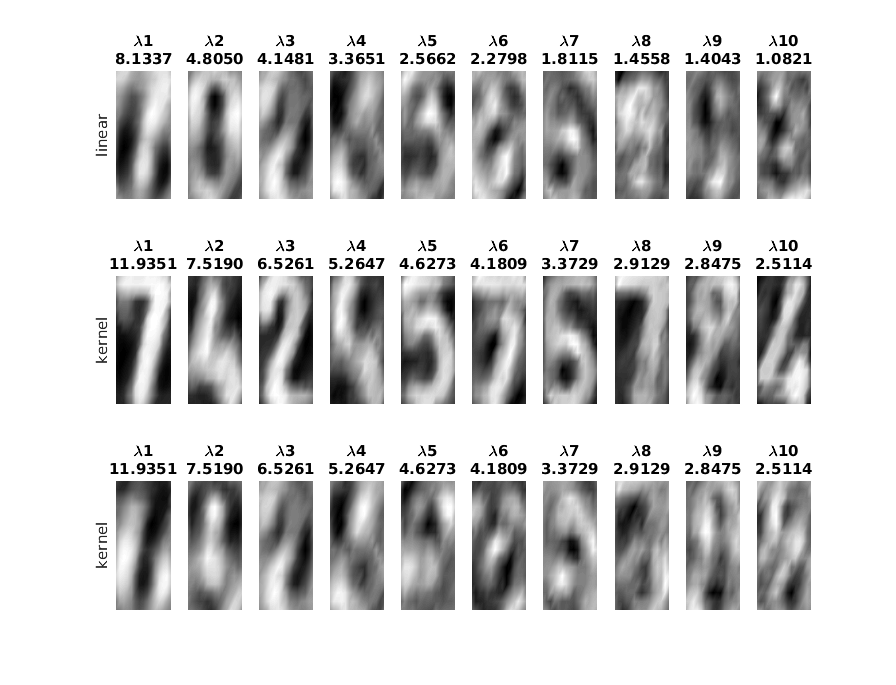
\includegraphics[width=0.7\linewidth]{../src/figure/pcKerLin}
\caption{The principal components using linear PCA (first row). Kernel PCA principal components (second row) and projections using the first principal components (third row).}
\label{fig:pcKerLin}
\end{figure}
\begin{figure}
\centering
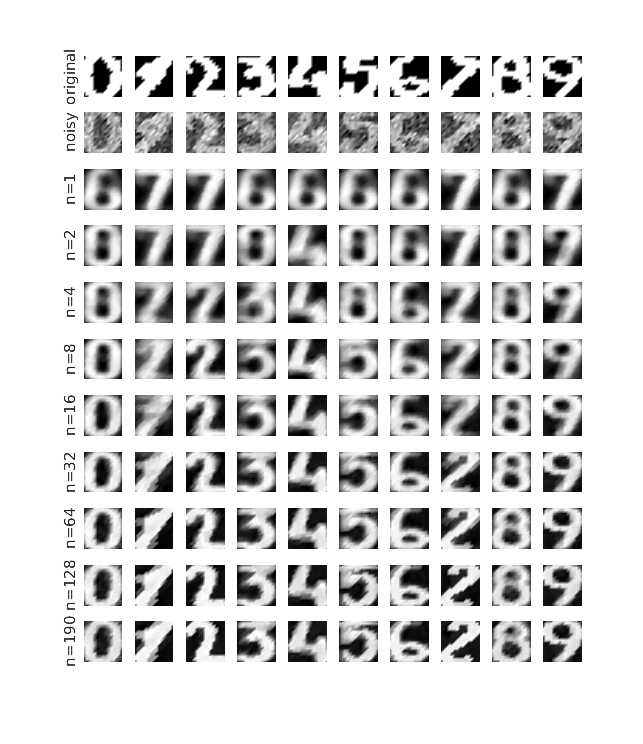
\includegraphics[width=0.49\linewidth]{../src/figure/denoise1}
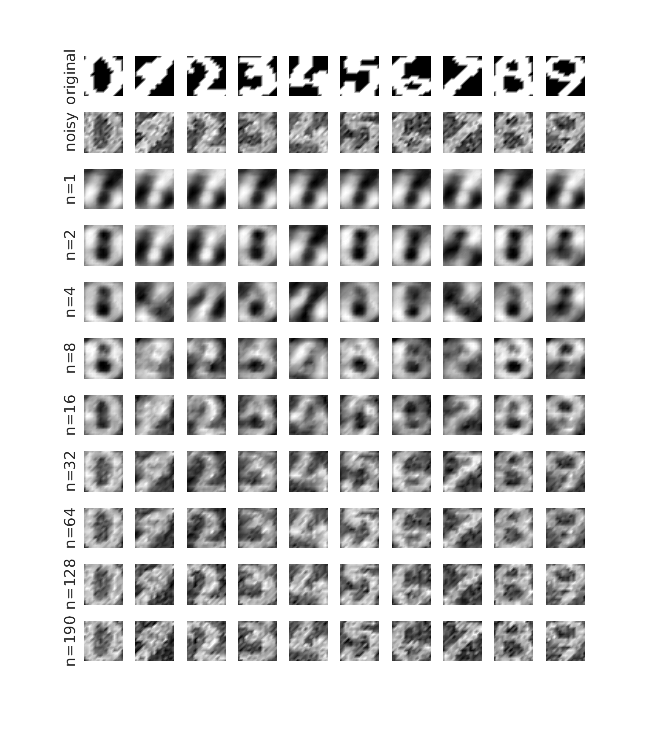
\includegraphics[width=0.49\linewidth]{../src/figure/denoise2}
\caption{Digit de-noising using kernel (left) and linear PCA (right).}
\label{fig:denoise2}
\end{figure}
\begin{figure}
\centering
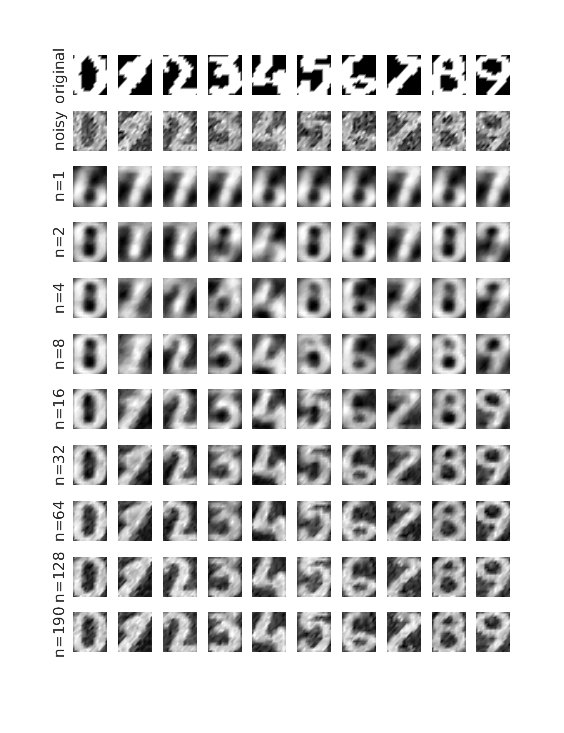
\includegraphics[width=0.49\linewidth]{../src/figure/denoiseKerLargSigm}
\caption{The kernel pca process using an rbf function with larger width $\sigma^2$.}
\label{fig:denoiseKerLargSigm}
\end{figure}
The miss-representation of the number seven in the can be fixed by increasing the rbf-kernel width, the result is shown in figure~\ref{fig:denoiseKerLargSigm}. Unfortunately increasing the width also increases the noise, so a good trade off is required. 

\section{Spectral clustering}
In this section a problem consisting of two interlocked rings as shown in figure~\ref{fig:interlock} will be analyzed. Two the human eye the grouping of points into two independent rings is immediately apparent. Spectral clustering is an algorithm, with which a computer can find these two classes. As the data set does not have annotations, this is an unsupervised learning algorithm. Spectral clustering methods use a kernel function as a similarity measure. The largest eigenvectors of a rescaled kernel-matrix are computed. The eigenvectors corresponding to the three largest eigenvalues are computed the second largest will contain the clustering information in the sign. If more then three eigenvectors are found the one containing the clustering information will be the smallest with an even number, if one starts counting with one at the largest vector. It must be noted that in this case the eigenvalues are all very close to one, so this observation cannot necessarily be generalized.  Figure~\ref{fig:clusteringResults} shows the results of using classification information from the second largest eigenvector when computing the first three eigenvectors using Lanczos' iterative method. It can be observed that for the two smaller values $\sigma^2 = 0.001$ and $\sigma^2 = 0.01$ the method is able classify the two rings correctly. For the larger value $\sigma^2 = 0.1$ the rbf-kernel becomes to large, which results in incorrect linear looking classification.  

\begin{figure}
\centering
% This file was created by matlab2tikz.
% Minimal pgfplots version: 1.3
%
%The latest updates can be retrieved from
%  http://www.mathworks.com/matlabcentral/fileexchange/22022-matlab2tikz
%where you can also make suggestions and rate matlab2tikz.
%
\documentclass[tikz]{standalone}
\usepackage{pgfplots}
\usepackage{grffile}
\pgfplotsset{compat=newest}
\usetikzlibrary{plotmarks}
\usepackage{amsmath}

\begin{document}
\definecolor{mycolor1}{rgb}{0.00000,0.44700,0.74100}%
%
\begin{tikzpicture}

\begin{axis}[%
width=2.0in,
height=2.0in,
scale only axis,
xmin=-1,
xmax=1,
tick align=outside,
xmajorgrids,
ymin=-1,
ymax=1,
ymajorgrids,
zmin=-0.2,
zmax=1,
zmajorgrids,
view={-130.7}{27.6},
axis x line*=bottom,
axis y line*=left,
axis z line*=left
]
\addplot3 [color=mycolor1,only marks,mark=*,mark options={solid}]
 table[row sep=crcr] {%
-0.373861205682992	0.828884557291946	0.507279353461388\\
0.444026554342783	0.304297700210832	0.511956556253337\\
0.312993850257902	0.110675267782329	0.487697461514205\\
0.484978346369727	0.304914956003247	0.47735337095752\\
-0.400455150671451	0.806885398426707	0.51727534695152\\
0.40707403230632	0.760284014950369	0.522537174485052\\
-0.436723305157612	0.25734667588341	0.498588606367124\\
0.277443195465818	0.913421838864534	0.50848824784811\\
0.407941593589588	0.807183414421151	0.508556393010679\\
-0.0829852285026614	0.0041594123297963	0.494035003808728\\
-0.50624369363082	0.687489536939812	0.487799933334246\\
-0.0902562819549997	0.0148183786686413	0.484060422095125\\
0.0199926698626982	0.00048971550127311	0.505865951731258\\
-0.226901485789117	0.0346236077046749	0.487372126649171\\
-0.121240250992492	0.00358542259754748	0.514363937237801\\
-0.19562665571718	0.042687918133734	0.510757682053917\\
-0.290291558022365	0.907773909633709	0.51993840885386\\
0.347998501134409	0.868489692265228	0.478428334233655\\
0.323456165456817	0.135738652771862	0.47860589669355\\
-0.0955246515747005	0.989442736482378	0.517337284040021\\
0.00839766630210372	0.000401259231602739	0.48931473950546\\
-0.372957352290681	0.208701642065911	0.505658621413584\\
0.42103639973477	0.715859087036311	0.509692767570455\\
0.0787334285565358	0.989585837511091	0.493609340457226\\
0.177494717016693	0.978963782379872	0.499079728927637\\
0.434829276855818	0.33135268360881	0.482380608529107\\
0.0782953171918924	0.00222878401084895	0.488751659341356\\
0.276872896280993	0.0651105617918381	0.476741231844547\\
0.13913656135004	0.989366093806526	0.50582032134855\\
0.0487867606923529	0.998780218806966	0.489639138246983\\
-0.178868255596047	0.0249230639639852	0.484454907698268\\
-0.445574041573537	0.572403950944119	0.501038999599728\\
-0.513781100007374	0.473093372831973	0.512718495453155\\
-0.387300875207209	0.771445683592876	0.488481600376413\\
0.46589245844946	0.444927685933116	0.485776396056322\\
-0.49376283102292	0.610654560032904	0.511527730598746\\
0.478626035423362	0.728396489058849	0.475733145445644\\
0.441821752602733	0.375353056245478	0.520358806661705\\
0.185666397365567	0.0246430493433864	0.49796264400776\\
0.463691501528025	0.572666006856834	0.482847428989742\\
-0.425408650662683	0.688628132785458	0.477158790845006\\
-0.489564633835686	0.467080016678043	0.502895553122932\\
-0.475070651131357	0.648037435102557	0.487342600527584\\
0.384758060068754	0.8129522287214	0.511587294188689\\
0.44531506866573	0.33351473346135	0.476379090387431\\
0.156090592499925	0.0319063926479003	0.521910670558248\\
0.490596568306627	0.31131473615358	0.523756966010293\\
-0.456088091781295	0.777596575680322	0.494744539289441\\
-0.23644918446544	0.0455436047230447	0.502135683235096\\
-0.41380693530715	0.190913842002509	0.491204402002334\\
-0.454282246862549	0.71034724480527	0.475403449368741\\
-0.437374384154497	0.258942597324141	0.518120887416227\\
0.0539075146521694	0.99603726243763	0.477037518231676\\
-0.172360049145152	0.963226557169321	0.507984077572476\\
0.187298350058122	0.0242282949719949	0.493910602491782\\
-0.158935223956579	0.0336675061987233	0.511808934962959\\
0.146623716818912	0.0288659159460513	0.50105680953126\\
0.304465430100499	0.873038991142308	0.52362155856799\\
0.349316022525647	0.851242592751898	0.515838876595851\\
-0.473685484181338	0.501822224504851	0.499607304997959\\
0.109741947757863	0.00282493132796824	0.502969185030065\\
-0.509520259879914	0.613546172065784	0.517205288922591\\
0.349401590286988	0.191853915938968	0.511412768915775\\
-0.49566724026478	0.538959065750753	0.498671699878575\\
0.388593784159521	0.825913362013532	0.477973267108167\\
-0.348648033058796	0.176735563536954	0.513711524369038\\
-0.157711756563664	0.958640510165817	0.501635542592347\\
0.0397457226972775	0.00440730937890997	0.522507457580835\\
0.369084330256097	0.173335928874408	0.510946285440196\\
0.272765689357211	0.926453713538913	0.515594232696509\\
0.4828611534862	0.66879110828708	0.484236404092475\\
0.423800165981472	0.317993326230099	0.476550355742932\\
0.107425090281239	0.0128855389509286	0.524767071023351\\
-0.355242554082385	0.143503719906681	0.495484627666378\\
-0.407560703110568	0.271237415928795	0.482505032657593\\
0.490163791991992	0.324523390547694	0.489411417877203\\
-0.0531147324092611	-0.00219908365869111	0.506508500820622\\
-0.281020979655332	0.0962329121441635	0.478038882930814\\
-0.328034176192459	0.159105600447764	0.488300496147565\\
-0.304707155726078	0.925329813272326	0.486935375031059\\
0.215476783570035	0.967759997076393	0.503601998094778\\
0.464633524819806	0.580539080068372	0.483555733702258\\
-0.400354549429377	0.232942874239531	0.482913905263272\\
-0.544929878740073	0.446369750531166	0.5035297456242\\
0.0283369937197632	-0.00194295382000684	0.498116776584414\\
-0.0806649967270442	0.0116515683313402	0.49350201286647\\
-0.507543424082448	0.348425170102414	0.509310161556645\\
0.470240255054822	0.522949370395302	0.497275117979131\\
-0.277646804430144	0.933429943893382	0.505949204237987\\
-0.164559223986932	0.973543972593209	0.495440418651437\\
-0.506477682426254	0.435635895099555	0.479628478394484\\
0.435526750707921	0.719992963640182	0.50299285054031\\
-0.505592728476442	0.694366226792276	0.488925301315417\\
0.342569828974748	0.894673292795709	0.523785467486081\\
-0.382738752671683	0.80643098079869	0.509925097686464\\
0.146999114483435	0.0159617827504373	0.50352392198061\\
0.353250271509765	0.140561291514195	0.510509029090859\\
0.21115223081577	0.954452652761708	0.509065961510603\\
-0.120224846295031	0.987793935698527	0.50631829780767\\
-0.468296867262678	0.372648562831454	0.484721090280262\\
0.0278372834005184	0.997859761690953	0.480558409235717\\
0.10364468266261	0.979984158081189	0.477074159432863\\
-0.167300498678857	0.980038286218673	0.513229754685835\\
0.522727192314501	0.539609608478908	0.489092942254664\\
-0.455118682894251	0.352191563912925	0.511939256839659\\
-0.533088563808675	0.513352713674409	0.485986815103356\\
0.330811558543946	0.892250088128073	0.506647940278537\\
0.0341613025991171	0.997567723895325	0.486236125456905\\
-0.31665760457379	0.0755667299174428	0.489401352477246\\
0.218354084434508	0.946282550694793	0.513196278162516\\
-0.344600700471244	0.114419649861457	0.482080369742428\\
0.274013739325898	0.110673678920507	0.518225106729547\\
-0.245175390675885	0.920483804148603	0.484521978307965\\
0.368270139337644	0.867561090782014	0.499961854380045\\
-0.389181888608762	0.157287279371152	0.512947571138043\\
0.314575147799708	0.0777583477069129	0.52093046434063\\
0.271433877439561	0.0519239315866734	0.493171312183611\\
0.518040940391632	0.602560834165858	0.476167965927257\\
-0.0425703199023117	0.998908920838019	0.519607522551435\\
-0.327496498629783	0.861202766999163	0.494735602311061\\
0.194792442483036	0.0390564636142438	0.50434002502739\\
0.528949629587177	0.416281895594809	0.504095544826443\\
0.329112579881509	0.149835344291471	0.477627411595447\\
0.0792251656335928	0.0104752776820626	0.508817281588143\\
0.304828982400548	0.0712904147976316	0.509232226014904\\
0.446951415351019	0.635668886386704	0.490583938878123\\
-0.139776816831525	0.019424164107195	0.511901799058998\\
0.45068852844449	0.558103584900853	0.481235645572958\\
-0.111481367490334	0.0181164378379434	0.5083364499603\\
-0.475444111091006	0.738993380598972	0.501095136833354\\
-0.369154868747491	0.86833678544941	0.51559962764948\\
-0.154459647128026	0.9863198559236	0.481696978993703\\
0.260121498453634	0.0590124170012024	0.500100919483129\\
-0.0804350512907256	0.988397338530203	0.519804370526133\\
0.509700252624326	0.338490370887519	0.492876668395057\\
-0.458127068313809	0.334534302106351	0.499376801097783\\
-0.457953992623491	0.320569380360156	0.507030378439932\\
0.345696488129988	0.896017672567819	0.483047442556072\\
0.481231752490138	0.461661250794602	0.493398617958296\\
-0.501899237565617	0.542425991570102	0.496128794985335\\
-0.335914779247551	0.904012700553332	0.491654289802169\\
-0.262172763770091	0.0636983020345958	0.475516255325265\\
-0.0238110517348724	0.999465782867543	0.496873384979194\\
0.131118771861154	0.988075915106548	0.498005052701914\\
0.388891626009524	0.146079585966985	0.503311836970499\\
0.449996039057375	0.480325925036146	0.484539559893314\\
-0.334720530392453	0.841650387828159	0.49063948888542\\
0.468751585762544	0.757121763121219	0.524860768827595\\
0.487367641284123	0.65844332163414	0.490858249075762\\
0.0383856356029642	0.000970592473503955	0.496169116048806\\
-0.400356861743489	0.173662149488901	0.509777958849473\\
-0.321997673014192	0.0923826786704125	0.517574258151596\\
-0.295538947100961	0.0815165812734599	0.523184851263703\\
-0.356861699598834	0.872889636878367	0.517667547977794\\
0.378203112121713	0.148481411552149	0.484164312788522\\
-0.251888883474787	0.0586170487227165	0.517888982524168\\
0.407100673770943	0.198431421150218	0.48259478770827\\
0.494746568809445	0.623063215457125	0.518047329862936\\
0.465972186563024	0.718626774883499	0.519169214557281\\
-0.0631400023710319	-0.000642596759899103	0.524875710428062\\
0.310622563597491	0.857590983809473	0.485258748067819\\
-0.408740148219957	0.705398632402873	0.501367139221594\\
0.172756407338189	0.971604870710907	0.483868300981743\\
-0.261274692532713	0.0990381526266023	0.507748900730731\\
-0.506280100082392	0.412483555399039	0.481916948839158\\
-0.383692188826925	0.75681527135529	0.520730106597509\\
0.0627032775522165	0.998029354161384	0.501849030361628\\
0.0299876963830273	0.000684176904963964	0.49142554914333\\
0.44568912193951	0.603492958586467	0.504013831622808\\
0.216196161940464	0.963133339150798	0.485936736600499\\
0.0375829924295263	0.995025654721195	0.483838136170475\\
-0.315830111722709	0.913971011532953	0.51671512107479\\
-0.465177715192763	0.695707754253198	0.504197771205556\\
0.441765426031914	0.631570841481208	0.493442747483033\\
0.213349333553297	0.0458936843409033	0.47620842784704\\
0.409096891664604	0.764893970122845	0.504005575989825\\
-0.531653469183273	0.569472403147358	0.518016803891111\\
-0.414624970555825	0.762812360085506	0.491071499391975\\
-0.185076266590092	0.0510428032901244	0.481779900954171\\
-0.102447591062752	0.0106754217787075	0.514418793210851\\
0.168696911363485	0.951343635506814	0.513436093262544\\
0.429491995836666	0.326709922611876	0.486801795021552\\
0.0446634453407604	0.998925271313073	0.477818925437719\\
-0.500067165080772	0.43162524705067	0.499159116362216\\
0.318058103159603	0.876091262817486	0.502624984819671\\
-0.424841381902409	0.722057824636885	0.510828844183328\\
-0.432725884234301	0.295585488764406	0.514822269798909\\
-0.443355284742512	0.389929173768422	0.511303000757032\\
-0.0335313903246702	0.999221307318621	0.500760089500535\\
-0.318628121730094	0.108169013219366	0.516904260016125\\
0.264263168220065	0.90757471673381	0.522985183776819\\
0.4494941060369	0.231341755219036	0.494542563020467\\
0.398439979409278	0.746280111817034	0.504846968733575\\
-0.528798804014779	0.370078588880022	0.490592278696567\\
0.508810802389621	0.405493078057688	0.482845180001462\\
-0.490782395331002	0.506872559366888	0.518419108186507\\
0.441396817056941	0.225136617322674	0.509910685746787\\
-0.166806334770739	0.957481708960037	0.481316057359473\\
-0.501409261772018	0.514568179242656	0.522508105483097\\
0.481219472774268	0.339881398187237	0.485340294509798\\
-0.422482489771265	0.193297001923687	0.516733605160018\\
0.510940275786233	0.404755851870785	0.499658999060897\\
0.15777743019768	0.975737201033196	0.475390490953508\\
-0.18355493879314	0.968749827248661	0.524949464069623\\
-0.0315591833374618	-0.00133479850755233	0.480421081874389\\
0.535341145848858	0.517593695557787	0.512015049746199\\
-0.0161302663036771	0.999101433157523	0.494989291207633\\
0.527705302956552	0.473852591085587	0.520401651131095\\
-0.0131602654424717	-0.000806017530978467	0.510183420162529\\
0.083790255709869	0.990330004008066	0.501680417542427\\
-0.447279743047677	0.321240405748184	0.512826949044618\\
-0.219662704387665	0.938622135458219	0.520344567578314\\
-0.381109155511121	0.152980625811269	0.497224867641127\\
0.446464399395966	0.218081203810897	0.497447007327437\\
-0.449212131166369	0.407424026329991	0.483058609687018\\
-0.384660240675413	0.241723273359221	0.48145568329469\\
0.335727437026755	0.154187255886173	0.476370909614509\\
-0.130932484588841	0.0085782442046175	0.489323748723826\\
0.0898305515237768	0.00293694039322895	0.520467704549281\\
-0.317796472101205	0.0772674203627145	0.496138419912701\\
-0.334360181760132	0.163964366305717	0.479564514119899\\
-0.457892886820382	0.572787297529019	0.52175136039094\\
0.257009918873448	0.895301687645055	0.478684157938643\\
-0.527000634946486	0.37473647099712	0.491061617662752\\
-0.310663476068535	0.859648032186165	0.522183185962358\\
-0.299822289799602	0.104733432288906	0.48489393760973\\
-0.41708580148539	0.756674776398153	0.500962241767521\\
-0.530797596157364	0.543808468288611	0.476307558520371\\
-0.043155930977164	0.0011735816843757	0.476883309951684\\
-0.405582919569552	0.832247151612451	0.516087849317501\\
-0.403470188124356	0.795454917444359	0.479634168140612\\
0.289863204637977	0.122194286506596	0.481938111521198\\
0.472550539422407	0.426468723404982	0.492697170911771\\
0.0882904678863488	-0.000557528348384452	0.505375932011454\\
0.414604409430035	0.808528301264059	0.489466206022538\\
0.42338467463001	0.784216791401532	0.50990771141677\\
0.274173347591385	0.94279654781676	0.49770888901899\\
-0.0462899655510212	0.995789698703355	0.518049865071235\\
0.104105447865323	0.989300326425113	0.522319182445618\\
0.412584005355157	0.83165099523561	0.487126788960584\\
0.0683216036991119	0.00210442884834148	0.510596695039691\\
0.330364797628189	0.12229569051131	0.503386888620275\\
-0.412362039711254	0.74061816670852	0.476990565890132\\
-0.509466526078424	0.343365093537333	0.520624295878456\\
-0.458508725525188	0.612811514234453	0.475678582063154\\
-0.321249367273474	0.128208922973481	0.49937706389439\\
-0.463163289580691	0.282101062391909	0.475007456259722\\
0.0376150271068693	0.992978811676176	0.483905214651178\\
-0.223830838283066	0.935302873111749	0.516323443114807\\
-0.0713385711963469	0.00525027101741679	0.511607947382665\\
-0.141916445850961	0.973698139077214	0.482058287829502\\
0.191694528360174	0.973832011609522	0.511776343796967\\
0.518477245454978	0.451888963866229	0.495219107589617\\
-0.438664780696935	0.220476194041925	0.481147518413713\\
0.431734116697412	0.224870838013633	0.487701192799851\\
-0.33240077466914	0.875178380836161	0.492851116166984\\
-0.527763024742615	0.421564583420859	0.492307636395598\\
-0.451671919003914	0.775112745212515	0.492153605030587\\
0.137749415137685	0.00772522887217969	0.483081213216752\\
0.224412016865696	0.0735430634371788	0.511953496379139\\
-0.0215797764381246	-0.000695328473043609	0.515633909556023\\
0.412323619299885	0.732539010773118	0.524541877762626\\
-0.266946375440358	0.932025342402598	0.523168562249813\\
0.13157172015602	0.989343997394985	0.479310444832281\\
-0.0515689507485599	-0.000290398641698081	0.509599822489119\\
-0.538863839098416	0.432920561633081	0.479645436163536\\
-0.352320995221312	0.798893682682456	0.507850129485528\\
0.439390150252401	0.354622924559081	0.511844470557569\\
0.416272739043605	0.754364782684221	0.476717814370067\\
0.432437889347285	0.182112380149897	0.497928697434421\\
-0.0451127830923892	0.998981582745863	0.478261166014618\\
0.346916465368262	0.825787564440974	0.502848032799468\\
0.495115810297701	0.374811860123211	0.498317443797658\\
-0.463608127682226	0.264759850268991	0.510452179227612\\
0.238336663403205	0.0603574555868909	0.517877712728148\\
0.523404864952893	0.411314785241895	0.508867926019519\\
0.402570756483139	0.223323893842404	0.505689129474145\\
-0.399060029360598	0.252118870529633	0.499288434187204\\
0.409362536170305	0.701825584950349	0.512688294413921\\
0.342510486230874	0.185292234452249	0.518909965871659\\
-0.39450971267982	0.841677948346444	0.478131058517852\\
0.499618886568163	0.484752760325463	0.520056998056694\\
0.0699213833343257	0.00173264142155635	0.476476082726365\\
-0.526596790208803	0.529485035102429	0.520004636504239\\
-0.439381862245734	0.760108199565904	0.495022370782328\\
0.508839605886128	0.515435899446998	0.494489414366872\\
0.399747638656227	0.849770219781594	0.518691060895577\\
-0.146222623359108	0.98620867893586	0.486103676178575\\
-0.270830486488434	0.942067335513253	0.51122812589192\\
0.210903637652526	0.0496764137776637	0.483468894419388\\
-0.340819454490219	0.898828190087624	0.485577988242475\\
-0.377323824204196	0.132974879541184	0.502477630316442\\
0.290465209416042	0.931485927498331	0.497775443610592\\
0.123994102326043	0.990983054480796	0.479323495738307\\
0.505424078022213	0.52831877279009	0.522970790718187\\
-0.00456853552587765	0.999931283808849	0.481814523793589\\
0.445246076532693	0.700005223032218	0.480961512311854\\
0.469635789636471	0.504038671756185	0.489260001689212\\
-0.246864301017331	0.913532633703051	0.482656920867406\\
-0.426382744995588	0.726442228144266	0.508531547606766\\
-0.185054204792877	0.0448968363747178	0.498951579574113\\
-0.251457061502565	0.0934666801692864	0.497889115776665\\
0.546952091180883	0.483558290368622	0.515069105983384\\
0.449494329677425	0.353039925037282	0.507046279447521\\
0.376978997286385	0.19515471221735	0.480214011332345\\
0.446832099773703	0.764944945276155	0.522518395650715\\
-0.375190013233378	0.225674315625118	0.508254389089877\\
0.216089857201755	0.932857176230501	0.513235185812833\\
-0.282875331216132	0.0591973114090647	0.475790513539246\\
-0.509743415954545	0.517623890911976	0.492673495881251\\
-0.499277513505764	0.386289441478959	0.511794411402502\\
0.27281593502893	0.940832820781544	0.509797553575325\\
-0.298713728459723	0.859532188483258	0.493046273529294\\
-0.195526693147743	0.049885560408639	0.519116425332579\\
-0.295145541573981	0.113112283827171	0.484846363533378\\
-0.0923241207533068	0.01160400295452	0.477612275987376\\
0.495451029914429	0.333422662908138	0.489420709762874\\
0.382068113395867	0.767453916264634	0.494068493410195\\
0.0151910608713463	0.999360071445961	0.496514780277496\\
0.383303143525145	0.840744490013217	0.509789114424787\\
-0.464415690974686	0.223740318955516	0.524327745957354\\
-0.313179312552607	0.858045853591608	0.492435772007795\\
0.416966964310859	0.691584149762922	0.498433516693657\\
0.386560743138598	0.196264663565518	0.522414190127875\\
-0.0330664695405201	0.00273294764595333	0.486713331583788\\
0.183399680032625	0.950792036097097	0.503204133840828\\
0.0406633331139483	0.99834016056557	0.48245201146968\\
0.512479190418318	0.530949892039179	0.482307596782023\\
0.472699814472699	0.290896656652694	0.487013964966523\\
0.215855322531842	0.0733500577498862	0.476014037471085\\
0.0482583579401082	0.00354574964466828	0.50782229100549\\
-0.195492939291588	0.973660012133807	0.518228231384963\\
-0.480660264526946	0.671480874592356	0.521797163867796\\
0.116876089723616	0.0171720343771697	0.480740374222773\\
-0.369660338113035	0.864469190029982	0.509600338601737\\
-0.39176432516321	0.214827838882464	0.503147249667787\\
0.256551650469205	0.0985385714313994	0.515451436118846\\
-0.101086658930327	0.00819117420265325	0.517788108515566\\
0.493857264704415	0.347594094456225	0.479579963576126\\
-0.270123892625973	0.892638699033501	0.498956664096624\\
-0.313044924660836	0.90590842563199	0.501772606956786\\
-0.111233395066662	0.985611872671711	0.497271556467245\\
-0.281519392865476	0.0994280922147489	0.496026771750178\\
0.0800590735677687	0.98540491825913	0.487249615503223\\
-0.00158704090879117	-0.000133583180892236	0.486655980778723\\
0.497861328644562	0.463871765415462	0.49813757274546\\
-0.00317103723283549	-0.00030111522933773	0.48099639100226\\
-0.491131835359482	0.656780028015917	0.48952209628946\\
0.458418209396981	0.209829899364053	0.478478354325021\\
0.399230645936135	0.14845645572398	0.522149064679535\\
-0.273093465242382	0.051386253111599	0.476954446848408\\
0.420429107709393	0.668248097921049	0.508681536416795\\
0.244467427880741	0.0795367013808713	0.492418624428554\\
-0.479833695525903	0.359800615665878	0.522511875276338\\
-0.0910136039647885	0.991998211586293	0.518963834263436\\
-0.0725374463909634	0.00921153194115236	0.499524836776668\\
0.34115440447378	0.145587317228142	0.504375961610209\\
0.486610818893923	0.643305606430475	0.475040423512893\\
0.425158738648267	0.787556980981965	0.47886413843082\\
-0.522547298751674	0.484490608316665	0.475765803402289\\
-0.324340140252556	0.14125397490796	0.486682915981155\\
0.422702886149167	0.206908184125364	0.478047112116748\\
0.0599130695177338	0.00247106738679265	0.486276717587126\\
0.390215887113671	0.861532898419356	0.496879794607897\\
0.358809330607673	0.877993441154307	0.515846341688852\\
-0.282890365230488	0.896050588681844	0.514089315638486\\
-0.35891942893614	0.10469290346884	0.510707740835594\\
0.209279510970648	0.940556464531694	0.486992917292828\\
-0.543851640560439	0.45871529818741	0.499209312701538\\
-0.151464135109467	0.018476484147842	0.512116105548892\\
0.299984276053998	0.866335601469739	0.480722422586126\\
0.219584865099716	0.055239992593756	0.504809520157885\\
-0.282135546123115	0.881144648632089	0.50206955974691\\
-0.446754988901948	0.751082971554425	0.522586742603658\\
-0.392969992730278	0.143403222783483	0.492910411738824\\
-0.253856121332303	0.0569121253294356	0.501203023350599\\
-0.360132872462445	0.126370198331403	0.488932269890908\\
-0.182039722427426	0.970682915009582	0.498435900386578\\
0.291042356265049	0.0914063374631162	0.502126850873119\\
-0.420310216934098	0.82061101812486	0.50554090650679\\
0.248162179756678	0.0935121827552815	0.494408193730443\\
0.39081068583956	0.841448193801115	0.504399822264761\\
-0.504262984105033	0.608751036775588	0.481779598592793\\
-0.474088678779437	0.682962944462954	0.480544687955642\\
-0.501725135949098	0.442892621889336	0.494839211375669\\
0.415897410863976	0.235667969152324	0.47841392339358\\
0.454140690688854	0.258762772337641	0.492160486312875\\
0.236480730157101	0.0727020172978582	0.519708813530546\\
-0.031391176755662	0.998134509367419	0.512573671715764\\
-0.472116520703201	0.428777105461353	0.519555555969733\\
0.155710102541175	0.0252600076672988	0.492995619736908\\
-0.521083119491365	0.496241649709949	0.503034943131919\\
-0.520894807657472	0.649105303276286	0.48792725668524\\
-0.298463490917857	0.868200979640417	0.504679943700706\\
-0.505410817446914	0.365084440901771	0.520853646130663\\
0.0922177879070745	0.979079862439979	0.505549720724592\\
-0.174482411984346	0.950715838845502	0.477521216667528\\
0.474615092497775	0.673565667574651	0.495471749685025\\
0.533749670340584	0.468735598227532	0.477706376758605\\
-0.0563643195935065	0.997198082197652	0.505638642590806\\
-0.0129212719311495	0.270815786873869	0.0467697444733335\\
0.0158516118224664	-0.527567779459346	0.433465659487805\\
-0.0124067004910065	0.319764245570998	0.147810563506006\\
-0.0084491021130095	-0.436603288609899	0.319419021967432\\
-0.00136140316889287	0.253574087065363	0.937458988067022\\
0.011160862010216	-0.411306082484556	0.268074333859679\\
-0.0230932608803687	-0.240428186454274	0.962077638991801\\
-0.00308074167816241	-0.423575003894358	0.747230004800323\\
-0.000988599929687575	0	0\\
0.01383262301422	-0.148887379037881	0.971105393052478\\
-0.000374266444898824	0.472562793792868	0.37806744320344\\
0.0157652767929712	0.417235540454084	0.654367291428653\\
-0.0201274600112654	0.415690435098179	0.151742561273228\\
0.0164728918002659	-0.343506676859842	0.117663341752638\\
0.0178360813434397	-0.142870463158897	0.971707329101116\\
0.0137816504024931	-0.505841144735098	0.592519168917025\\
-0.0221203284243254	0.439921000245658	0.631619527065537\\
0.0210100038552256	0.348999767701628	0.815049966302943\\
-0.0130574420010431	-0.020657118168989	0.999728326759533\\
-0.0151428744418778	-0.221112117741357	0.958821033891795\\
0.00118741364792045	0.455934516401966	0.383720020827762\\
0.0178682094672773	0.0978488547617722	0.993344834372625\\
-0.00740591258991013	-0.161676886454882	0.0159527669707832\\
0.0204448071708186	0.555569382811347	0.431212943165538\\
-0.00827033513098351	-0.37708052004472	0.18442372969839\\
-0.0222666113896015	-0.0356032531329716	0.999289212082244\\
-0.0192210185376683	-0.181789921440989	0.95934386411463\\
0.0122584076387706	-0.156573807021287	0.0370180551243291\\
-0.00543710439327398	0.0282694639883208	0.00275639047190547\\
0.0241787068643753	-0.343542044883354	0.894788278803597\\
-0.00884220109901114	-0.111583147493401	0.0174786101540353\\
0.0070994594844534	-0.500156466113716	0.383121526591316\\
0.0144710072725092	0.365460333537105	0.104794921655628\\
-0.016793796224634	0.104092830781316	0.983156646099565\\
0.0236141763234266	0.163600261657576	0.966154626951381\\
0.0240530496308006	-0.209596456699169	0.0661374443252364\\
0.00249953206206102	-0.382668446671539	0.121614499558446\\
0.0123312436743315	-0.258227209773576	0.0727006342058011\\
-0.0225051256996181	-0.100266509682433	0.0152392580074298\\
0.00774134498703324	-0.521971679870426	0.667909639147961\\
0.0138023801846093	-0.271606005048007	0.0655987702294471\\
-0.0232108724320149	-0.361936713159376	0.805092592719584\\
0.0158387786541794	0.2085872683017	0.92196433772386\\
-0.00491804984051065	-0.468259413679759	0.700181174812252\\
0.00536985617431306	-0.47088208477969	0.356200408896973\\
-0.0166508865763025	-0.24045254828634	0.944067945702998\\
-0.019528092027505	0.069093262130652	0.0108684415546305\\
-0.0144641292992512	-0.0707571423566049	0.996723274552155\\
0.0130253325191528	0.433570455065131	0.18304476805281\\
0.0206210833363732	-0.427514801159874	0.72677139652449\\
0.0169412097963773	-0.0814377532093431	-0.00323930451919333\\
0.015535220214854	-0.17819231339088	0.97294207483793\\
0.0232624979765357	-0.298158577468723	0.0775967462658513\\
0.0239421428052751	0.392866403971725	0.845193969690359\\
0.0201723210508637	0.281095408332408	0.0912006796005248\\
-0.0162117116611346	0.237027781446706	0.0708981655423186\\
0.0161648188031573	-0.39058860742282	0.232021941616447\\
-0.0226065560662668	0.051311815145262	0.984112934556206\\
0.0023047109473993	-0.472502817242981	0.494520485950098\\
-0.0179994221444796	-0.175567193996453	0.955531677277937\\
-0.00514266290654378	0.200906425329057	0.969277378645483\\
0.00923953379788209	0.398921830947384	0.21138282373047\\
0.00437740451482965	0.467549933683599	0.344962196904348\\
0.0124504623909153	0.136757137874161	0.0182226719327805\\
-0.0224698203136124	-0.300308288247752	0.844605342618185\\
-0.0104641707294139	0.472525724501669	0.22343092662249\\
-0.0150599082703043	-0.206611929508126	0.97339734109683\\
0.0175028825279168	-0.047243001133217	0.986222948230102\\
-0.0134685143753753	-0.281941469264165	0.924561369641165\\
-0.00951059640958853	0.242656018128777	0.951396033190465\\
-0.00467610333142824	0.352287719522402	0.13899035338116\\
-0.0218607426611468	0.428112831138712	0.76563707362833\\
-0.0171857891902725	0.307476057899291	0.102285668937684\\
0.0103252871025935	0.41993286147724	0.209341441187674\\
0.0176734170312958	0.494138280119794	0.270490275485369\\
-0.0152880876207774	0.0307691298137865	0.993214514267982\\
-0.00556909478060325	-0.285396908191375	0.921209154575368\\
0.00488422681716484	-0.456078883470515	0.499829295594925\\
0.00115686801401396	0.464062366808045	0.29150704109743\\
-0.0161500717913755	-0.45181318144708	0.369435507860902\\
-0.000926122162383536	0.225808652695006	0.0313720194648615\\
0.0106377161162669	0.497446746294162	0.685325402754416\\
-0.0210304781638873	0.393936963537182	0.71825378128803\\
0.00668416681560403	0.526607398543245	0.656321617862072\\
-0.0115366905387746	0.147710204346335	0.00672411328355887\\
-0.0177578328516704	0.304860643573809	0.071154899712771\\
0.00915135027621706	-0.120934910851504	0.0217431830876567\\
-0.0152470130448856	0.535789047529907	0.526642519831771\\
-0.00649536091354558	0.530112301253885	0.6000402021024\\
0.00678593468594751	0.277749486698172	0.945214517349246\\
0.0188149476849013	0.0499790633303956	-0.00010290579879529\\
-0.00639145913269453	0.202731836222209	0.929756048441095\\
0.00903614712395317	0.430321857007354	0.660753491288271\\
0.0136041879655432	-0.373992092913548	0.879853354931902\\
0.0049145543606787	0.432231371614402	0.660675560601987\\
-0.0218267121803668	0.0515655621978446	0.995273024622334\\
-0.0167640341527569	0.0970639840746013	0.995060881620921\\
-0.0163964345826923	-0.102996287482609	0.00111279356299978\\
0.00703484821584447	0.475862661592857	0.719232770714003\\
-0.0212269169345885	0.496861820572592	0.629065068875867\\
0.0175090619975809	-0.372159545485112	0.834159002457559\\
-0.0151207321556844	-0.312191684051552	0.125541896541174\\
-0.00510167411389366	-0.13643194312656	0.98761072234213\\
0.00767608197247253	0.355106783912833	0.215580876321862\\
-0.00077705923387594	0.297051236726149	0.0624340667967979\\
-0.00827256539503591	-0.366370839954083	0.827623909424848\\
0.000177536253743948	-0.530972638332401	0.485645394982834\\
-0.020017527798034	-0.0415260454784718	0.00213050118778363\\
-0.0100939341224589	-0.526810187018743	0.518266174714338\\
0.000783782977233172	0.284419965638333	0.939439291540602\\
-0.00726124955064918	-0.073119684416329	0.000212604047954848\\
0.00376444592417913	0.402584730977453	0.288865333592154\\
0.00506353957341441	-0.323977205064543	0.14208442069739\\
0.00879058944613581	0.4957638035601	0.722742049671365\\
-0.0182676883403918	0.196717915884119	0.0641130833180648\\
0.0230860368233311	-0.381187303219442	0.791741472454552\\
-0.00578001861100782	-0.422640175207103	0.669160537018854\\
-0.00823459079861083	-0.134944189528827	0.978342398010718\\
-0.00129368850416921	-0.182228395377656	0.941450251716102\\
0.00169646971686135	0.175751266003426	0.0245846441623822\\
-0.00268580146950436	-0.435785661111667	0.714486139550275\\
-0.00673799788748267	-0.381979948595918	0.150793166816892\\
0.014729119330426	-0.504675411122612	0.592199821955066\\
0.00173504896289123	-0.34764217336037	0.884089872850211\\
0.00934063665341209	-0.276997416193832	0.0824330401637526\\
0.0234771435134911	-0.292380388899027	0.896549105736808\\
-0.000967993782848217	0.123990894949608	0.0320043844014122\\
-0.00241029103004997	-0.270009432685835	0.940193335347282\\
-0.0211248003194081	0.326714756067945	0.151496391749615\\
0.00592427125021821	0.531504365680034	0.426772197347968\\
0.00117203207084904	0.0299844838826321	0.000812870647824949\\
0.0200685306190542	-0.141451780239116	0.97405135253318\\
0.00594933572251069	0.300744126648995	0.90601719228229\\
-0.00632407265080294	0.281082555298928	0.118546905380773\\
0.0189673216844963	0.291004358195437	0.93321036988109\\
0.0158932415088208	-0.23751095597024	0.0745858457684234\\
-0.00567850622160842	0.466879950323691	0.267917493458106\\
0.000165991457901765	0.552006237212377	0.412191547234831\\
0.0176604059124288	0.487919555206116	0.406879371712654\\
-0.0117227011224565	-0.24360672100125	0.958414698756155\\
-0.0194702113944782	0.273357929085031	0.108214834054972\\
-0.00487912068747145	0.47616669023305	0.725043678279061\\
-0.00110455071502717	0.440942263984962	0.278125201095129\\
-0.0237934795645883	-0.0222299801805556	0.997467562984284\\
0.000918459143579398	0.515686668165873	0.670638265208071\\
-0.0138089351619959	0.11386309495987	0.97294919017985\\
0.008881645653089	-0.453026262015175	0.690425999483643\\
0.0128796858112484	-0.539467182819367	0.595499621764454\\
0.0222701047404088	-0.38816179114838	0.827548765026577\\
-0.00359413092750126	-0.250385511841813	0.958151488278269\\
-0.0165478454394477	0.0153432482595085	0.995905805396326\\
0.00475575914608656	-0.415202043233573	0.277937537333967\\
-0.00555536143159944	0.116547267452011	0.0192777997500467\\
0.000406830885557952	-0.502082657313306	0.505667711254073\\
-0.002333077987953	0.334175595006898	0.0768477589754027\\
0.0247121269078962	0.524192071050271	0.63574591403326\\
-0.0118748616378739	-0.552043880530063	0.427826965152536\\
-0.0216355225228591	0.400813606624124	0.190888382106483\\
0.00761397503681845	0.0730623933743696	0.980983781586005\\
-0.0152126162678534	0.175984983606077	0.982999079507918\\
-0.00848948382054872	-0.453292828436832	0.338868804216974\\
-0.00732515625835103	0.108761446690643	0.0149071475626851\\
-0.0181450142909751	0.320561776613283	0.866609914955037\\
0.0183795447657495	-0.0897358778800509	0.994827811896439\\
0.000875526145199901	0.0764685679910257	0.993800133053634\\
0.010939744395211	-0.363653140133604	0.143343308338621\\
-0.00261782680707695	0.349844786254324	0.891853695454793\\
-0.00443390532589506	0.145926495890149	0.959736776267248\\
-0.00235145526907266	0.265355536888144	0.923006051173048\\
-0.00899787182566891	0.0196992751635632	0.991053608120946\\
0.00457215971982975	0.175686050533297	0.979289984339855\\
0.00888804007294856	0.452765781307598	0.582705633871125\\
-0.000160781606240235	0.504840571659637	0.319027259635275\\
0.0117462367134899	0.192276237886026	0.049993513008727\\
0.0113289141411178	0.517840677243285	0.356681510659728\\
0.023093215244553	0.388125997270629	0.791964508906798\\
0.00925737748317854	0.164517602854793	0.959482209981331\\
0.0225306313859588	-0.519329158314513	0.328257450758788\\
0.0240453039789437	0.096390523288018	0.019017181524965\\
0.0248653773381798	0.449506175658111	0.492604616437143\\
-0.00344327898558664	-0.441773568990437	0.415478025603549\\
-0.0241072825034766	-0.411222518973883	0.171039802062482\\
0.00656072303117057	0.436727738701295	0.705351163030866\\
0.00943609502823269	-0.454764118078852	0.414957857376139\\
-0.0123189595902032	0.240304256629229	0.945669041078539\\
0.0109182339146773	-0.445672725689822	0.489206877035014\\
0.0049159753451425	0.252017628507509	0.0422891209005221\\
0.0106645687458732	-0.415993350568527	0.701145685036631\\
0.00306809427783621	-0.240992266006617	0.950138276661664\\
0.00968017949444031	0.0780333772174981	0.996241371424727\\
-0.0197190860970908	-0.434902917889584	0.18708073552374\\
0.00482974262026724	-0.483379717600226	0.74958706432558\\
0.0173069006146476	-0.430884645439851	0.173763078472345\\
-0.0211466310350736	0.208620897668495	0.0640428719375501\\
-0.00234182696094238	0.312743335428409	0.111381198337377\\
-0.00500495751634546	-0.448109011157003	0.72054657368089\\
-0.0104688234738318	0.485221448143558	0.468213983162948\\
-0.00457329823529926	0.36028881790397	0.17053258940611\\
-0.015834391706588	-0.372942827651214	0.820723113649166\\
0.0128972129356735	-0.417969056153557	0.778327692435339\\
0.0163123331582677	0.357486674995793	0.87562015212946\\
0.0188605651363015	-0.188864623858131	0.0243092262918549\\
-0.00489237628849288	0.0267489138479462	0.99945773291036\\
-0.0100506574873522	0.00995848335936893	0.000908446967237394\\
0.013372042086184	0.0747449007738303	0.996676738235213\\
-0.0160650962985051	-0.405510091930576	0.31828168293552\\
-0.00523414531597707	-0.060357083226127	0.991255936196956\\
-0.00575153892260148	-0.355870147332951	0.895890425838045\\
0.0178140496045297	-0.039973910100057	0.996693701601217\\
-0.0133867694000486	-0.316521622629659	0.865296610943132\\
-0.0235402693039489	0.130644390830336	0.969098149745705\\
0.0155693033075756	0.0599053582286482	0.00265143896105501\\
0.0158602207050685	0.1503407601216	0.954416584395389\\
-0.022494328154539	0.352483010752497	0.20499832733513\\
0.0119048955447633	-0.545396178589708	0.434441310941579\\
0.0244927798244964	0.310538554617753	0.917173235892571\\
-0.0100499830582391	0.178331992070014	0.057245013721632\\
-0.00779944065716039	-0.535178935413351	0.501332914440227\\
-0.0203859105861696	-0.376528777276843	0.742223130378136\\
0.00595766039770703	-0.406259843063056	0.823289946722195\\
-0.000139987711374062	0.242266042584517	0.910267497895644\\
0.0215092167007853	-0.492801527728159	0.656666618286349\\
0.0229560980453466	-0.249777889531842	0.895360646908502\\
0.00388228948744707	0.443583026992268	0.727545310777846\\
0.0116784529299577	-0.179104018989784	0.0231681324027786\\
0.0119339427780986	-0.490801369751841	0.454968132968527\\
-0.0100697353390251	-0.318174348985302	0.865348603266272\\
-0.0038760039939063	0.406876938909867	0.697568091381231\\
-0.00873480206337059	-0.211778023795041	0.968996233412164\\
0.00699511323101332	-0.366453966547262	0.236971832317637\\
-0.0246479449055562	0.461162832518731	0.702817907597918\\
0.0111630694301381	-0.29298237960535	0.0574494501418215\\
0.00886279533639306	0.350506755563231	0.842077007661243\\
0.00714545156040151	0.516914821497938	0.344125941206886\\
-0.0112736532720387	0.488736789612864	0.604133140361712\\
0.01176647567749	-0.352597830508284	0.119815752242998\\
0.0236146833283658	0.261989442329416	0.041116029637654\\
0.0175471113349365	0.481852299581482	0.520410920557043\\
0.0124601724725528	0.337507722894605	0.83367777225824\\
-0.0111770416089134	0.455000853645252	0.477244558704465\\
0.0114009292828283	-0.460924789984008	0.635805837474732\\
-0.00937418849487281	-0.0722700521260137	0.992612386766726\\
-0.015798295062685	0.388852783992595	0.249065291329362\\
-0.0126472412203647	-0.394969781937273	0.849395488722782\\
0.0043593806826968	0.478961425067741	0.299026881832958\\
-0.00609435435979653	0.219370007531633	0.929566804556931\\
-0.00367772100445567	-0.496283715727373	0.566817562404918\\
0.00293993828537858	0.164565958518995	0.946637240924216\\
0.0188034091642813	-0.190398445943662	0.961875242082256\\
-0.00160734136262755	0.519198561064976	0.323732810967519\\
-0.00639042482757617	0.431833232819749	0.821820539037404\\
-0.0180778748653703	-0.192121322294199	0.0617142964839102\\
-0.0116384814533579	0.458349890009099	0.634006979507952\\
-0.00283281286486755	0.345295053151175	0.83516584517775\\
0.0179697518200742	-0.431085497589702	0.169444509133851\\
0.00111395892404765	0.0032421686839165	0.997601112865739\\
-0.0098478517963905	0.362235309616325	0.787294456370273\\
0.00572371956704	0.14469382369827	0.98084318501102\\
0.0222521982879993	-0.2677323909185	0.893957653406167\\
-0.0154239256308782	-0.474589438023203	0.732888849158242\\
0.0101152577035988	-0.539270147959559	0.368306843180715\\
0.0239600765559549	0.177241243944529	0.0252414263865691\\
0.00679420081268105	-0.411709957442777	0.729624980958413\\
0.0162430734920251	-0.519881728675162	0.595467858161623\\
0.0129811428621377	-0.0914098518755163	0.00316540025965508\\
-0.0212348675766714	-0.0328847806773336	0.00441039799942569\\
-0.0212940512799539	-0.153078112313561	0.986535215950542\\
-0.0220045002641379	-0.391217695376096	0.175597923772497\\
-0.00212383649304588	-0.524058518928389	0.601175905391472\\
-0.000405454732756552	-0.507790311660209	0.387889148860568\\
-0.00808685786885248	-0.17009376124215	0.0149766310183415\\
-0.00579243384541788	-0.548233802576328	0.534048594299953\\
-0.000102917780956666	-0.243258570474194	0.0597494628293724\\
0.0122480381231756	0.0382147873410891	0.00374554386818716\\
-0.0109880116650821	-0.451431707935939	0.764802692232066\\
0.0153497693686293	-0.0650326522901391	0.991913626266075\\
0.0208456151650465	-0.184585182614066	0.0527911221889929\\
0.012599143096977	-0.0702122043381784	0.983215411741604\\
-0.00213791217594918	0.492951494156215	0.375596298861162\\
-0.00797098399865623	-0.00318170940409939	-0.000151237499429228\\
-0.00313538945268059	-0.0512220325067857	0.00597866193661168\\
0.0194232308249673	0.464740245715061	0.719424092064263\\
-0.0223469815367072	0.438903782595794	0.461023919091176\\
0.00446308394292638	-0.51315447957226	0.393483890425386\\
-0.0128925120927756	0.390266806455	0.278461248372814\\
-0.0202857038513214	-0.237014599434988	0.0326239357529515\\
0.00821889303131763	0.0659937731788768	0.997664625990281\\
-0.00377818677816974	-0.435409790820738	0.444514242092133\\
-0.0249667206033395	0.3247602877132	0.0757917947338345\\
0.014335230368518	0.141469142380125	0.982581072649493\\
-0.0114624779937056	-0.0686617860978832	0.991841750705462\\
0.0221865895582375	-0.433164821365431	0.800246032255445\\
-0.0197282147244407	0.138581325963082	0.0163553336538432\\
-0.0141216104998871	0.453732836162598	0.546560412966627\\
0.0221424043493869	0.055672816466033	0.998420057393521\\
-0.0184604639756163	-0.156225150990856	0.948495502389488\\
-0.00822477793492223	0.403296588845152	0.159062527724841\\
-0.000517226413154986	-0.202981388232421	0.0596840323984507\\
0.0222339425017474	0.26455820373648	0.0798836737326158\\
-0.0172388076606477	0.0253140478513819	0.998780981626941\\
-0.00242298607127761	-0.438884673871439	0.760395383309637\\
-0.00705862519371952	0.290567808227417	0.856464685272497\\
0.0104975330594167	0.299070459811796	0.0975140047675948\\
0.0215994127730887	0.4405738362564	0.582133923627273\\
-0.00941528923461281	0.434535870463919	0.255645102933788\\
0.00554106196378661	-0.460751597073642	0.356113677312775\\
0.011793059655759	-0.305608678682722	0.0864050508563707\\
0.0146448694154273	-0.502240620523102	0.280938200156901\\
-0.00857813637356279	-0.399520195660114	0.179109061810484\\
0.00594902671675411	-0.150251737757286	0.0151411529478018\\
-0.00646145129349487	-0.448674496902287	0.543033813645528\\
0.00729389577131227	0.441706740758385	0.631611886062196\\
0.0103777525036521	-0.0615518105029911	0.000484513411035769\\
0.00627027730293188	0.502904792205354	0.412795153748148\\
-0.018459445859875	-0.110419927991375	0.0144483164445947\\
0.00537014184213249	-0.429433687138952	0.736949233951632\\
-0.0241485259856376	-0.350722786158013	0.888881573152575\\
-0.0195566961645107	-0.420458218257849	0.787422863706692\\
-0.000989800740766597	0.190400623444663	0.977361825254692\\
0.00171550556902487	-0.421069701824592	0.661703692407998\\
0.0244726326062039	0.0250711065431452	0.998475032876945\\
-0.0177274524123015	-0.138667814837919	0.0261933923517655\\
-0.00567651947247809	0.461698800399636	0.389295350745044\\
0.000129458922278458	0.417890122583691	0.781132216810128\\
-0.00927445785243184	-0.241352100384897	0.921993396565572\\
-0.00531150623308733	0.205701824546212	0.935202703700421\\
-0.0192866927792378	-0.092915801153639	0.00500500283887088\\
0.0220767127075811	0.535886058588978	0.453691021498569\\
0.0105837360556797	-0.519534807191816	0.486084268257683\\
-0.0139756844784457	-0.507931895207694	0.43393947242188\\
-0.00732537358226756	0.507351779902618	0.56155515164047\\
0.0203930359922376	-0.457609900001608	0.622702282514032\\
0.00255387297847091	-0.464893600153217	0.427049773009195\\
-0.0161611289890546	-0.400999666641078	0.802500191626957\\
-0.0249097513923787	0.485015079917175	0.466731935369067\\
-0.0205433832160966	-0.556537882387065	0.496328368054505\\
0.00294003990514708	-0.358824514926253	0.785095776423672\\
-0.0198582150321491	0.512564343126843	0.631603180475447\\
-0.00743077021460653	-0.451858006486754	0.742288246185582\\
-0.0158082062952995	0.469999024250261	0.777634713388989\\
-0.0140798911840784	0.493440048319496	0.491040924132826\\
0.00858020333456009	-0.502037854449347	0.523584283836432\\
0.0214539851943225	-0.433783756300526	0.350489345648787\\
-0.0150882690399284	0.452818136845114	0.348766506457554\\
0.00776252463242632	0.374975974189633	0.840936788356882\\
-0.018403963345106	0.40683678452372	0.837915891398308\\
-0.0190286398408644	-0.258279228144128	0.880331893152203\\
0.0223611969840765	0.490709493115726	0.586005902138063\\
-0.0155049928112081	-0.121162575197349	0.00562886200507747\\
0.0165153659440764	0.396595667974812	0.753245165456793\\
-0.0233520299907171	0.0799090413040815	0.000950489373494505\\
0.00554254243800529	0.432767743320966	0.203032333357566\\
-0.020425627936579	-0.433640411468426	0.207717068692045\\
0.00171786493326392	0.370890410095867	0.227234063387485\\
-0.0151380948727095	0.018327057801709	-0.0017061908587852\\
-0.00292698583560348	0.216745500431979	0.0655008229345998\\
-0.0214129365263582	-0.199023696568062	0.0219457281962659\\
-0.0208782787307547	-0.435162763545305	0.242689170591841\\
-0.0210411117993755	0.232272789660681	0.050516232971223\\
-0.0216689010221755	-0.351255734757206	0.903632123732661\\
-0.0108758922212684	0.39792662646778	0.846154668335921\\
-0.00449400151679002	-0.406861346335422	0.304649742296994\\
0.00283423719127724	0.360205279357217	0.187979999782576\\
0.0214765525858876	-0.512516945020772	0.462092917060716\\
0.00280768790354167	-0.512705041209437	0.326276031197629\\
-0.0110908580614199	-0.22867459472961	0.0332396445616851\\
0.0243849292201437	0.412346595539573	0.258711280110418\\
-0.0139690775890095	-0.504320785122036	0.309496161616563\\
0.0083462798815208	0.0199864261990984	0.000699597955272574\\
0.000186528764361599	-0.415359646655664	0.259136694525867\\
0.0128874565473673	-0.450610935922264	0.52416050423496\\
-0.00808626159242501	0.0781962010510534	0.00452529706530806\\
-0.0122833912711076	0.0968399476132462	0.98913919563265\\
-0.0168488600354314	-0.137814140702026	0.976307280507641\\
0.0133695313420437	-0.123911862713174	0.990527570857065\\
0.0215685685843584	-0.170995463646285	0.0213315639320423\\
0.00830394033756908	0.398884670164236	0.860527534916273\\
0.00156335725231385	-0.446290325795119	0.659804135073725\\
0.000112048089121231	0.28746701696396	0.919677710310691\\
-0.0077718762460584	0.475013875426296	0.435176109985798\\
0.0218847908027715	-0.152017967648637	0.0131644294560097\\
-0.0127158285035678	-0.262773785162224	0.0611716402956098\\
0.00154987644512268	0.321318753442549	0.835320423567231\\
-0.0162565721339149	-0.347451447391462	0.784629658656065\\
0.0203008027478428	0.44379257901278	0.621028612147915\\
-0.0201190835867165	-0.304257171717703	0.0856320788136164\\
-0.0132114760396992	0.127521752252401	0.023306943927092\\
0.00516151555217386	0.551514125189842	0.398591378513723\\
-0.0194882566270019	0.0481272544595166	0.00502083955202722\\
0.0109542999277477	-0.386475322009279	0.134510453639048\\
0.0178712952830454	0.149390684301722	0.00376548550126837\\
-0.0170851413897623	-0.457658207955485	0.217953026010202\\
-0.0164203956758051	0.451884166981728	0.414382641775743\\
0.0185066903670066	0.50693954290865	0.505984204422717\\
0.012138816256518	0.221282139208653	0.0824836369269479\\
-0.0217322253898427	-0.326144193283837	0.110620185669212\\
-0.0076468011696646	0.439188289263068	0.232386570089131\\
-0.00745279336133942	0.454244091627237	0.476310544341506\\
-0.0138032799890596	-0.510271046611822	0.627128291483398\\
0.0225934323571688	-0.501635167406495	0.406138518114136\\
};
 \end{axis}
\end{tikzpicture}%
\end{document}
\caption{The training data set consisting of two interlocked rings.}
\label{fig:interlock}
\end{figure}



\begin{figure}
\centering
% This file was created by matlab2tikz.
% Minimal pgfplots version: 1.3
%
%The latest updates can be retrieved from
%  http://www.mathworks.com/matlabcentral/fileexchange/22022-matlab2tikz
%where you can also make suggestions and rate matlab2tikz.
%
\documentclass[tikz]{standalone}
\usepackage{pgfplots}
\usepackage{grffile}
\pgfplotsset{compat=newest}
\usetikzlibrary{plotmarks}
\usepackage{amsmath}

\begin{document}
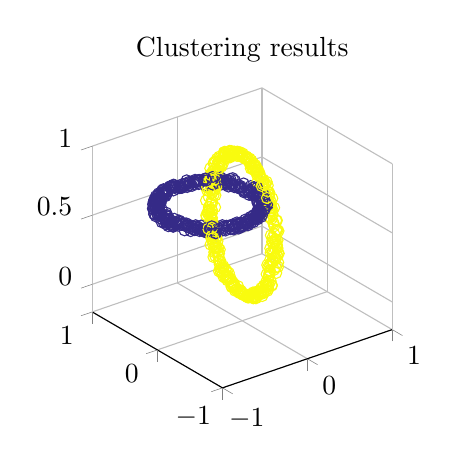
\begin{tikzpicture}

\begin{axis}[%
width=1.5in,
height=1.5in,
scale only axis,
colormap={mymap}{[1pt] rgb(0pt)=(0.2081,0.1663,0.5292); rgb(1pt)=(0.211624,0.189781,0.577676); rgb(2pt)=(0.212252,0.213771,0.626971); rgb(3pt)=(0.2081,0.2386,0.677086); rgb(4pt)=(0.195905,0.264457,0.7279); rgb(5pt)=(0.170729,0.291938,0.779248); rgb(6pt)=(0.125271,0.324243,0.830271); rgb(7pt)=(0.0591333,0.359833,0.868333); rgb(8pt)=(0.0116952,0.38751,0.881957); rgb(9pt)=(0.00595714,0.408614,0.882843); rgb(10pt)=(0.0165143,0.4266,0.878633); rgb(11pt)=(0.0328524,0.443043,0.871957); rgb(12pt)=(0.0498143,0.458571,0.864057); rgb(13pt)=(0.0629333,0.47369,0.855438); rgb(14pt)=(0.0722667,0.488667,0.8467); rgb(15pt)=(0.0779429,0.503986,0.838371); rgb(16pt)=(0.0793476,0.520024,0.831181); rgb(17pt)=(0.0749429,0.537543,0.826271); rgb(18pt)=(0.0640571,0.556986,0.823957); rgb(19pt)=(0.0487714,0.577224,0.822829); rgb(20pt)=(0.0343429,0.596581,0.819852); rgb(21pt)=(0.0265,0.6137,0.8135); rgb(22pt)=(0.0238905,0.628662,0.803762); rgb(23pt)=(0.0230905,0.641786,0.791267); rgb(24pt)=(0.0227714,0.653486,0.776757); rgb(25pt)=(0.0266619,0.664195,0.760719); rgb(26pt)=(0.0383714,0.674271,0.743552); rgb(27pt)=(0.0589714,0.683757,0.725386); rgb(28pt)=(0.0843,0.692833,0.706167); rgb(29pt)=(0.113295,0.7015,0.685857); rgb(30pt)=(0.145271,0.709757,0.664629); rgb(31pt)=(0.180133,0.717657,0.642433); rgb(32pt)=(0.217829,0.725043,0.619262); rgb(33pt)=(0.258643,0.731714,0.595429); rgb(34pt)=(0.302171,0.737605,0.571186); rgb(35pt)=(0.348167,0.742433,0.547267); rgb(36pt)=(0.395257,0.7459,0.524443); rgb(37pt)=(0.44201,0.748081,0.503314); rgb(38pt)=(0.487124,0.749062,0.483976); rgb(39pt)=(0.530029,0.749114,0.466114); rgb(40pt)=(0.570857,0.748519,0.44939); rgb(41pt)=(0.609852,0.747314,0.433686); rgb(42pt)=(0.6473,0.7456,0.4188); rgb(43pt)=(0.683419,0.743476,0.404433); rgb(44pt)=(0.71841,0.741133,0.390476); rgb(45pt)=(0.752486,0.7384,0.376814); rgb(46pt)=(0.785843,0.735567,0.363271); rgb(47pt)=(0.818505,0.732733,0.34979); rgb(48pt)=(0.850657,0.7299,0.336029); rgb(49pt)=(0.882433,0.727433,0.3217); rgb(50pt)=(0.913933,0.725786,0.306276); rgb(51pt)=(0.944957,0.726114,0.288643); rgb(52pt)=(0.973895,0.731395,0.266648); rgb(53pt)=(0.993771,0.745457,0.240348); rgb(54pt)=(0.999043,0.765314,0.216414); rgb(55pt)=(0.995533,0.786057,0.196652); rgb(56pt)=(0.988,0.8066,0.179367); rgb(57pt)=(0.978857,0.827143,0.163314); rgb(58pt)=(0.9697,0.848138,0.147452); rgb(59pt)=(0.962586,0.870514,0.1309); rgb(60pt)=(0.958871,0.8949,0.113243); rgb(61pt)=(0.959824,0.921833,0.0948381); rgb(62pt)=(0.9661,0.951443,0.0755333); rgb(63pt)=(0.9763,0.9831,0.0538)},
xmin=-1,
xmax=1,
tick align=outside,
xmajorgrids,
ymin=-1,
ymax=1,
ymajorgrids,
zmin=-0.2,
zmax=1,
zmajorgrids,
view={-37.5}{30},
title={Clustering results},
axis x line*=bottom,
axis y line*=left,
axis z line*=left
]
\addplot3[scatter,only marks,scatter src=explicit,scatter/use mapped color={mark=o,mark options={},draw=mapped color}] plot table[row sep=crcr,meta index=3]{%
0.34115440447378	0.145587317228142	0.504375961610209	-1\\
-0.0203859105861696	-0.376528777276843	0.742223130378136	1\\
-0.0151380948727095	0.018327057801709	-0.0017061908587852	1\\
0.481231752490138	0.461661250794602	0.493398617958296	-1\\
0.342510486230874	0.185292234452249	0.518909965871659	-1\\
-0.0122833912711076	0.0968399476132462	0.98913919563265	1\\
-0.00212383649304588	-0.524058518928389	0.601175905391472	1\\
-0.463608127682226	0.264759850268991	0.510452179227612	-1\\
0.0178682094672773	0.0978488547617722	0.993344834372625	1\\
0.449996039057375	0.480325925036146	0.484539559893314	-1\\
-0.0131602654424717	-0.000806017530978467	0.510183420162529	-1\\
-0.0139756844784457	-0.507931895207694	0.43393947242188	1\\
-0.501899237565617	0.542425991570102	0.496128794985335	-1\\
0.0215092167007853	-0.492801527728159	0.656666618286349	1\\
0.487367641284123	0.65844332163414	0.490858249075762	-1\\
-0.50624369363082	0.687489536939812	0.487799933334246	-1\\
-0.544929878740073	0.446369750531166	0.5035297456242	-1\\
-0.0130574420010431	-0.020657118168989	0.999728326759533	1\\
0.0128874565473673	-0.450610935922264	0.52416050423496	1\\
-0.0223469815367072	0.438903782595794	0.461023919091176	1\\
-0.449212131166369	0.407424026329991	0.483058609687018	-1\\
0.00283423719127724	0.360205279357217	0.187979999782576	1\\
0.0240453039789437	0.096390523288018	0.019017181524965	1\\
0.000918459143579398	0.515686668165873	0.670638265208071	1\\
-0.382738752671683	0.80643098079869	0.509925097686464	-1\\
-0.00827033513098351	-0.37708052004472	0.18442372969839	1\\
0.00594933572251069	0.300744126648995	0.90601719228229	1\\
-0.475070651131357	0.648037435102557	0.487342600527584	-1\\
0.0283369937197632	-0.00194295382000684	0.498116776584414	-1\\
-0.456088091781295	0.777596575680322	0.494744539289441	-1\\
-0.0515689507485599	-0.000290398641698081	0.509599822489119	-1\\
0.0049145543606787	0.432231371614402	0.660675560601987	1\\
-0.00884220109901114	-0.111583147493401	0.0174786101540353	1\\
0.0234771435134911	-0.292380388899027	0.896549105736808	1\\
0.0106645687458732	-0.415993350568527	0.701145685036631	1\\
0.0341613025991171	0.997567723895325	0.486236125456905	-1\\
0.0278372834005184	0.997859761690953	0.480558409235717	-1\\
-0.543851640560439	0.45871529818741	0.499209312701538	-1\\
-0.0226065560662668	0.051311815145262	0.984112934556206	1\\
-0.0139690775890095	-0.504320785122036	0.309496161616563	1\\
-0.00609435435979653	0.219370007531633	0.929566804556931	1\\
-0.00632407265080294	0.281082555298928	0.118546905380773	1\\
0.495451029914429	0.333422662908138	0.489420709762874	-1\\
-0.438664780696935	0.220476194041925	0.481147518413713	-1\\
-0.0150882690399284	0.452818136845114	0.348766506457554	1\\
0.402570756483139	0.223323893842404	0.505689129474145	-1\\
0.01383262301422	-0.148887379037881	0.971105393052478	1\\
-0.533088563808675	0.513352713674409	0.485986815103356	-1\\
-0.120224846295031	0.987793935698527	0.50631829780767	-1\\
0.0123312436743315	-0.258227209773576	0.0727006342058011	1\\
-0.35891942893614	0.10469290346884	0.510707740835594	-1\\
-0.439381862245734	0.760108199565904	0.495022370782328	-1\\
0.012138816256518	0.221282139208653	0.0824836369269479	1\\
0.407100673770943	0.198431421150218	0.48259478770827	-1\\
0.013372042086184	0.0747449007738303	0.996676738235213	1\\
-0.000926122162383536	0.225808652695006	0.0313720194648615	1\\
-0.432725884234301	0.295585488764406	0.514822269798909	-1\\
0.0124504623909153	0.136757137874161	0.0182226719327805	1\\
0.0247121269078962	0.524192071050271	0.63574591403326	1\\
-0.00649536091354558	0.530112301253885	0.6000402021024	1\\
-0.00578001861100782	-0.422640175207103	0.669160537018854	1\\
-0.00129368850416921	-0.182228395377656	0.941450251716102	1\\
-0.043155930977164	0.0011735816843757	0.476883309951684	-1\\
0.256551650469205	0.0985385714313994	0.515451436118846	-1\\
-0.0221203284243254	0.439921000245658	0.631619527065537	1\\
-0.372957352290681	0.208701642065911	0.505658621413584	-1\\
-0.022494328154539	0.352483010752497	0.20499832733513	1\\
0.527705302956552	0.473852591085587	0.520401651131095	-1\\
0.478626035423362	0.728396489058849	0.475733145445644	-1\\
-0.0104688234738318	0.485221448143558	0.468213983162948	1\\
0.00516151555217386	0.551514125189842	0.398591378513723	1\\
-0.121240250992492	0.00358542259754748	0.514363937237801	-1\\
0.0128796858112484	-0.539467182819367	0.595499621764454	1\\
0.472699814472699	0.290896656652694	0.487013964966523	-1\\
-0.00705862519371952	0.290567808227417	0.856464685272497	1\\
-0.0224698203136124	-0.300308288247752	0.844605342618185	1\\
-0.0233520299907171	0.0799090413040815	0.000950489373494505	1\\
0.014335230368518	0.141469142380125	0.982581072649493	1\\
0.454140690688854	0.258762772337641	0.492160486312875	-1\\
-0.335914779247551	0.904012700553332	0.491654289802169	-1\\
0.0214539851943225	-0.433783756300526	0.350489345648787	1\\
-0.0162565721339149	-0.347451447391462	0.784629658656065	1\\
0.523404864952893	0.411314785241895	0.508867926019519	-1\\
-0.0161302663036771	0.999101433157523	0.494989291207633	-1\\
-0.313044924660836	0.90590842563199	0.501772606956786	-1\\
-0.000374266444898824	0.472562793792868	0.37806744320344	1\\
-0.00823459079861083	-0.134944189528827	0.978342398010718	1\\
0.219584865099716	0.055239992593756	0.504809520157885	-1\\
0.508810802389621	0.405493078057688	0.482845180001462	-1\\
0.383303143525145	0.840744490013217	0.509789114424787	-1\\
0.384758060068754	0.8129522287214	0.511587294188689	-1\\
0.388593784159521	0.825913362013532	0.477973267108167	-1\\
-0.281519392865476	0.0994280922147489	0.496026771750178	-1\\
-0.49376283102292	0.610654560032904	0.511527730598746	-1\\
-0.0211466310350736	0.208620897668495	0.0640428719375501	1\\
0.00821889303131763	0.0659937731788768	0.997664625990281	1\\
0.449494329677425	0.353039925037282	0.507046279447521	-1\\
-0.334720530392453	0.841650387828159	0.49063948888542	-1\\
-0.328034176192459	0.159105600447764	0.488300496147565	-1\\
-0.00491804984051065	-0.468259413679759	0.700181174812252	1\\
0.00678593468594751	0.277749486698172	0.945214517349246	1\\
-0.0220045002641379	-0.391217695376096	0.175597923772497	1\\
-0.0109880116650821	-0.451431707935939	0.764802692232066	1\\
-0.527763024742615	0.421564583420859	0.492307636395598	-1\\
0.0103252871025935	0.41993286147724	0.209341441187674	1\\
-0.389181888608762	0.157287279371152	0.512947571138043	-1\\
-0.0038760039939063	0.406876938909867	0.697568091381231	1\\
-0.0192210185376683	-0.181789921440989	0.95934386411463	1\\
-0.39176432516321	0.214827838882464	0.503147249667787	-1\\
0.0130253325191528	0.433570455065131	0.18304476805281	1\\
-0.00449400151679002	-0.406861346335422	0.304649742296994	1\\
-0.520894807657472	0.649105303276286	0.48792725668524	-1\\
-0.000967993782848217	0.123990894949608	0.0320043844014122	1\\
0.0173069006146476	-0.430884645439851	0.173763078472345	1\\
0.0206210833363732	-0.427514801159874	0.72677139652449	1\\
-0.020425627936579	-0.433640411468426	0.207717068692045	1\\
-0.0100506574873522	0.00995848335936893	0.000908446967237394	1\\
0.008881645653089	-0.453026262015175	0.690425999483643	1\\
0.0699213833343257	0.00173264142155635	0.476476082726365	-1\\
-0.0237934795645883	-0.0222299801805556	0.997467562984284	1\\
0.21115223081577	0.954452652761708	0.509065961510603	-1\\
0.244467427880741	0.0795367013808713	0.492418624428554	-1\\
0.441821752602733	0.375353056245478	0.520358806661705	-1\\
-0.00283281286486755	0.345295053151175	0.83516584517775	1\\
-0.0172388076606477	0.0253140478513819	0.998780981626941	1\\
-0.0425703199023117	0.998908920838019	0.519607522551435	-1\\
-0.0165478454394477	0.0153432482595085	0.995905805396326	1\\
-0.522547298751674	0.484490608316665	0.475765803402289	-1\\
-0.00489237628849288	0.0267489138479462	0.99945773291036	1\\
-0.00732515625835103	0.108761446690643	0.0149071475626851	1\\
0.146623716818912	0.0288659159460513	0.50105680953126	-1\\
0.0165153659440764	0.396595667974812	0.753245165456793	1\\
0.0158602207050685	0.1503407601216	0.954416584395389	1\\
0.00488422681716484	-0.456078883470515	0.499829295594925	1\\
0.0109542999277477	-0.386475322009279	0.134510453639048	1\\
-0.501409261772018	0.514568179242656	0.522508105483097	-1\\
-0.472116520703201	0.428777105461353	0.519555555969733	-1\\
0.376978997286385	0.19515471221735	0.480214011332345	-1\\
-0.00514266290654378	0.200906425329057	0.969277378645483	1\\
-0.00359413092750126	-0.250385511841813	0.958151488278269	1\\
-0.0181450142909751	0.320561776613283	0.866609914955037	1\\
0.00293993828537858	0.164565958518995	0.946637240924216	1\\
-0.0218267121803668	0.0515655621978446	0.995273024622334	1\\
-0.245175390675885	0.920483804148603	0.484521978307965	-1\\
0.00171550556902487	-0.421069701824592	0.661703692407998	1\\
-0.399060029360598	0.252118870529633	0.499288434187204	-1\\
0.446464399395966	0.218081203810897	0.497447007327437	-1\\
0.44531506866573	0.33351473346135	0.476379090387431	-1\\
0.0218847908027715	-0.152017967648637	0.0131644294560097	1\\
0.0114009292828283	-0.460924789984008	0.635805837474732	1\\
-0.505410817446914	0.365084440901771	0.520853646130663	-1\\
0.00554106196378661	-0.460751597073642	0.356113677312775	1\\
0.0898305515237768	0.00293694039322895	0.520467704549281	-1\\
-0.425408650662683	0.688628132785458	0.477158790845006	-1\\
-0.130932484588841	0.0085782442046175	0.489323748723826	-1\\
-0.0108758922212684	0.39792662646778	0.846154668335921	1\\
0.0153497693686293	-0.0650326522901391	0.991913626266075	1\\
0.368270139337644	0.867561090782014	0.499961854380045	-1\\
-0.139776816831525	0.019424164107195	0.511901799058998	-1\\
0.508839605886128	0.515435899446998	0.494489414366872	-1\\
-0.0104641707294139	0.472525724501669	0.22343092662249	1\\
-0.412362039711254	0.74061816670852	0.476990565890132	-1\\
-0.015834391706588	-0.372942827651214	0.820723113649166	1\\
0.409096891664604	0.764893970122845	0.504005575989825	-1\\
-0.167300498678857	0.980038286218673	0.513229754685835	-1\\
-0.00779944065716039	-0.535178935413351	0.501332914440227	1\\
0.00154987644512268	0.321318753442549	0.835320423567231	1\\
-0.166806334770739	0.957481708960037	0.481316057359473	-1\\
0.0244726326062039	0.0250711065431452	0.998475032876945	1\\
0.00117203207084904	0.0299844838826321	0.000812870647824949	1\\
0.46589245844946	0.444927685933116	0.485776396056322	-1\\
-0.0212269169345885	0.496861820572592	0.629065068875867	1\\
0.00388228948744707	0.443583026992268	0.727545310777846	1\\
-0.0123189595902032	0.240304256629229	0.945669041078539	1\\
-0.00857813637356279	-0.399520195660114	0.179109061810484	1\\
-0.0214129365263582	-0.199023696568062	0.0219457281962659	1\\
0.0158387786541794	0.2085872683017	0.92196433772386	1\\
-0.0098478517963905	0.362235309616325	0.787294456370273	1\\
0.388891626009524	0.146079585966985	0.503311836970499	-1\\
-0.172360049145152	0.963226557169321	0.507984077572476	-1\\
0.458418209396981	0.209829899364053	0.478478354325021	-1\\
-0.261274692532713	0.0990381526266023	0.507748900730731	-1\\
-0.00235145526907266	0.265355536888144	0.923006051173048	1\\
-0.424841381902409	0.722057824636885	0.510828844183328	-1\\
0.260121498453634	0.0590124170012024	0.500100919483129	-1\\
0.441765426031914	0.631570841481208	0.493442747483033	-1\\
0.0146448694154273	-0.502240620523102	0.280938200156901	1\\
0.42338467463001	0.784216791401532	0.50990771141677	-1\\
0.000165991457901765	0.552006237212377	0.412191547234831	1\\
0.358809330607673	0.877993441154307	0.515846341688852	-1\\
-0.526596790208803	0.529485035102429	0.520004636504239	-1\\
0.0119339427780986	-0.490801369751841	0.454968132968527	1\\
0.172756407338189	0.971604870710907	0.483868300981743	-1\\
0.00886279533639306	0.350506755563231	0.842077007661243	1\\
0.0683216036991119	0.00210442884834148	0.510596695039691	-1\\
0.00537014184213249	-0.429433687138952	0.736949233951632	1\\
0.0162430734920251	-0.519881728675162	0.595467858161623	1\\
0.0800590735677687	0.98540491825913	0.487249615503223	-1\\
0.0043593806826968	0.478961425067741	0.299026881832958	1\\
-0.00797098399865623	-0.00318170940409939	-0.000151237499429228	1\\
0.216089857201755	0.932857176230501	0.513235185812833	-1\\
-0.0218607426611468	0.428112831138712	0.76563707362833	1\\
0.0599130695177338	0.00247106738679265	0.486276717587126	-1\\
0.0225934323571688	-0.501635167406495	0.406138518114136	1\\
-0.00457329823529926	0.36028881790397	0.17053258940611	1\\
0.330364797628189	0.12229569051131	0.503386888620275	-1\\
0.0240530496308006	-0.209596456699169	0.0661374443252364	1\\
0.0236146833283658	0.261989442329416	0.041116029637654	1\\
0.0179697518200742	-0.431085497589702	0.169444509133851	1\\
-0.295145541573981	0.113112283827171	0.484846363533378	-1\\
0.349401590286988	0.191853915938968	0.511412768915775	-1\\
0.44568912193951	0.603492958586467	0.504013831622808	-1\\
-0.0100697353390251	-0.318174348985302	0.865348603266272	1\\
0.000783782977233172	0.284419965638333	0.939439291540602	1\\
-0.369660338113035	0.864469190029982	0.509600338601737	-1\\
-0.0180778748653703	-0.192121322294199	0.0617142964839102	1\\
-0.195526693147743	0.049885560408639	0.519116425332579	-1\\
0.0175028825279168	-0.047243001133217	0.986222948230102	1\\
-0.0910136039647885	0.991998211586293	0.518963834263436	-1\\
0.0230860368233311	-0.381187303219442	0.791741472454552	1\\
-0.443355284742512	0.389929173768422	0.511303000757032	-1\\
-0.282875331216132	0.0591973114090647	0.475790513539246	-1\\
-0.18355493879314	0.968749827248661	0.524949464069623	-1\\
0.00830394033756908	0.398884670164236	0.860527534916273	1\\
-0.41708580148539	0.756674776398153	0.500962241767521	-1\\
-0.531653469183273	0.569472403147358	0.518016803891111	-1\\
0.0243849292201437	0.412346595539573	0.258711280110418	1\\
0.329112579881509	0.149835344291471	0.477627411595447	-1\\
0.00879058944613581	0.4957638035601	0.722742049671365	1\\
0.420429107709393	0.668248097921049	0.508681536416795	-1\\
0.484978346369727	0.304914956003247	0.47735337095752	-1\\
-0.0212940512799539	-0.153078112313561	0.986535215950542	1\\
0.0397457226972775	0.00440730937890997	0.522507457580835	-1\\
-0.00951059640958853	0.242656018128777	0.951396033190465	1\\
-0.0118748616378739	-0.552043880530063	0.427826965152536	1\\
-0.00937418849487281	-0.0722700521260137	0.992612386766726	1\\
0.0049159753451425	0.252017628507509	0.0422891209005221	1\\
0.0244927798244964	0.310538554617753	0.917173235892571	1\\
-0.0177274524123015	-0.138667814837919	0.0261933923517655	1\\
0.00656072303117057	0.436727738701295	0.705351163030866	1\\
0.0128972129356735	-0.417969056153557	0.778327692435339	1\\
-0.513781100007374	0.473093372831973	0.512718495453155	-1\\
-0.000517226413154986	-0.202981388232421	0.0596840323984507	1\\
0.465972186563024	0.718626774883499	0.519169214557281	-1\\
0.0221865895582375	-0.433164821365431	0.800246032255445	1\\
0.0222521982879993	-0.2677323909185	0.893957653406167	1\\
-0.0725374463909634	0.00921153194115236	0.499524836776668	-1\\
0.415897410863976	0.235667969152324	0.47841392339358	-1\\
-0.340819454490219	0.898828190087624	0.485577988242475	-1\\
-0.0225051256996181	-0.100266509682433	0.0152392580074298	1\\
0.493857264704415	0.347594094456225	0.479579963576126	-1\\
-0.0212348675766714	-0.0328847806773336	0.00441039799942569	1\\
0.299984276053998	0.866335601469739	0.480722422586126	-1\\
-0.00873480206337059	-0.211778023795041	0.968996233412164	1\\
0.399230645936135	0.14845645572398	0.522149064679535	-1\\
-0.400354549429377	0.232942874239531	0.482913905263272	-1\\
0.481219472774268	0.339881398187237	0.485340294509798	-1\\
0.216196161940464	0.963133339150798	0.485936736600499	-1\\
0.191694528360174	0.973832011609522	0.511776343796967	-1\\
0.0203930359922376	-0.457609900001608	0.622702282514032	1\\
0.0023047109473993	-0.472502817242981	0.494520485950098	1\\
-0.270830486488434	0.942067335513253	0.51122812589192	-1\\
0.431734116697412	0.224870838013633	0.487701192799851	-1\\
0.0113289141411178	0.517840677243285	0.356681510659728	1\\
0.00923953379788209	0.398921830947384	0.21138282373047	1\\
-0.33240077466914	0.875178380836161	0.492851116166984	-1\\
-0.00556909478060325	-0.285396908191375	0.921209154575368	1\\
-0.348648033058796	0.176735563536954	0.513711524369038	-1\\
-0.185054204792877	0.0448968363747178	0.498951579574113	-1\\
0.0204448071708186	0.555569382811347	0.431212943165538	1\\
0.505424078022213	0.52831877279009	0.522970790718187	-1\\
-0.0151207321556844	-0.312191684051552	0.125541896541174	1\\
-0.298713728459723	0.859532188483258	0.493046273529294	-1\\
0.00482974262026724	-0.483379717600226	0.74958706432558	1\\
0.512479190418318	0.530949892039179	0.482307596782023	-1\\
0.00925737748317854	0.164517602854793	0.959482209981331	1\\
-0.304707155726078	0.925329813272326	0.486935375031059	-1\\
-0.447279743047677	0.321240405748184	0.512826949044618	-1\\
0.000129458922278458	0.417890122583691	0.781132216810128	1\\
-0.000139987711374062	0.242266042584517	0.910267497895644	1\\
-0.0140798911840784	0.493440048319496	0.491040924132826	1\\
0.27281593502893	0.940832820781544	0.509797553575325	-1\\
0.469635789636471	0.504038671756185	0.489260001689212	-1\\
-0.315830111722709	0.913971011532953	0.51671512107479	-1\\
0.00592427125021821	0.531504365680034	0.426772197347968	1\\
0.0109182339146773	-0.445672725689822	0.489206877035014	1\\
-0.281020979655332	0.0962329121441635	0.478038882930814	-1\\
0.42103639973477	0.715859087036311	0.509692767570455	-1\\
-0.00213791217594918	0.492951494156215	0.375596298861162	1\\
-0.321997673014192	0.0923826786704125	0.517574258151596	-1\\
0.445246076532693	0.700005223032218	0.480961512311854	-1\\
0.107425090281239	0.0128855389509286	0.524767071023351	-1\\
0.304828982400548	0.0712904147976316	0.509232226014904	-1\\
-0.00579243384541788	-0.548233802576328	0.534048594299953	1\\
-0.00531150623308733	0.205701824546212	0.935202703700421	1\\
0.0220767127075811	0.535886058588978	0.453691021498569	1\\
0.0210100038552256	0.348999767701628	0.815049966302943	1\\
-0.509520259879914	0.613546172065784	0.517205288922591	-1\\
0.0299876963830273	0.000684176904963964	0.49142554914333	-1\\
-0.383692188826925	0.75681527135529	0.520730106597509	-1\\
0.390215887113671	0.861532898419356	0.496879794607897	-1\\
-0.403470188124356	0.795454917444359	0.479634168140612	-1\\
-0.490782395331002	0.506872559366888	0.518419108186507	-1\\
0.0158932415088208	-0.23751095597024	0.0745858457684234	1\\
0.00594902671675411	-0.150251737757286	0.0151411529478018	1\\
0.00627027730293188	0.502904792205354	0.412795153748148	1\\
-0.0111770416089134	0.455000853645252	0.477244558704465	1\\
-0.538863839098416	0.432920561633081	0.479645436163536	-1\\
0.414604409430035	0.808528301264059	0.489466206022538	-1\\
0.0787334285565358	0.989585837511091	0.493609340457226	-1\\
0.434829276855818	0.33135268360881	0.482380608529107	-1\\
0.224412016865696	0.0735430634371788	0.511953496379139	-1\\
-0.527000634946486	0.37473647099712	0.491061617662752	-1\\
0.0103777525036521	-0.0615518105029911	0.000484513411035769	1\\
0.0178140496045297	-0.039973910100057	0.996693701601217	1\\
0.0482583579401082	0.00354574964466828	0.50782229100549	-1\\
-0.00158704090879117	-0.000133583180892236	0.486655980778723	-1\\
-0.0114624779937056	-0.0686617860978832	0.991841750705462	1\\
0.137749415137685	0.00772522887217969	0.483081213216752	-1\\
0.15777743019768	0.975737201033196	0.475390490953508	-1\\
0.13913656135004	0.989366093806526	0.50582032134855	-1\\
0.0223611969840765	0.490709493115726	0.586005902138063	1\\
-0.219662704387665	0.938622135458219	0.520344567578314	-1\\
-0.327496498629783	0.861202766999163	0.494735602311061	-1\\
0.104105447865323	0.989300326425113	0.522319182445618	-1\\
-0.246864301017331	0.913532633703051	0.482656920867406	-1\\
-0.00292698583560348	0.216745500431979	0.0655008229345998	1\\
0.0188149476849013	0.0499790633303956	-0.00010290579879529	1\\
0.000112048089121231	0.28746701696396	0.919677710310691	1\\
0.472550539422407	0.426468723404982	0.492697170911771	-1\\
-0.0124067004910065	0.319764245570998	0.147810563506006	1\\
0.0232624979765357	-0.298158577468723	0.0775967462658513	1\\
0.00294003990514708	-0.358824514926253	0.785095776423672	1\\
-0.0335313903246702	0.999221307318621	0.500760089500535	-1\\
-0.437374384154497	0.258942597324141	0.518120887416227	-1\\
0.412323619299885	0.732539010773118	0.524541877762626	-1\\
0.510940275786233	0.404755851870785	0.499658999060897	-1\\
-0.000160781606240235	0.504840571659637	0.319027259635275	1\\
0.0144710072725092	0.365460333537105	0.104794921655628	1\\
-0.00344327898558664	-0.441773568990437	0.415478025603549	1\\
0.0070994594844534	-0.500156466113716	0.383121526591316	1\\
0.474615092497775	0.673565667574651	0.495471749685025	-1\\
0.210903637652526	0.0496764137776637	0.483468894419388	-1\\
-0.00827256539503591	-0.366370839954083	0.827623909424848	1\\
0.425158738648267	0.787556980981965	0.47886413843082	-1\\
-0.0152880876207774	0.0307691298137865	0.993214514267982	1\\
-0.0563643195935065	0.997198082197652	0.505638642590806	-1\\
0.318058103159603	0.876091262817486	0.502624984819671	-1\\
-0.0144641292992512	-0.0707571423566049	0.996723274552155	1\\
0.00714545156040151	0.516914821497938	0.344125941206886	1\\
-0.0161500717913755	-0.45181318144708	0.369435507860902	1\\
-0.318628121730094	0.108169013219366	0.516904260016125	-1\\
0.0199926698626982	0.00048971550127311	0.505865951731258	-1\\
-0.49566724026478	0.538959065750753	0.498671699878575	-1\\
-0.00510167411389366	-0.13643194312656	0.98761072234213	1\\
0.335727437026755	0.154187255886173	0.476370909614509	-1\\
0.494746568809445	0.623063215457125	0.518047329862936	-1\\
-0.400455150671451	0.806885398426707	0.51727534695152	-1\\
-0.146222623359108	0.98620867893586	0.486103676178575	-1\\
-0.475444111091006	0.738993380598972	0.501095136833354	-1\\
-0.464415690974686	0.223740318955516	0.524327745957354	-1\\
0.0178360813434397	-0.142870463158897	0.971707329101116	1\\
0.399747638656227	0.849770219781594	0.518691060895577	-1\\
0.0406633331139483	0.99834016056557	0.48245201146968	-1\\
-0.0100499830582391	0.178331992070014	0.057245013721632	1\\
0.0155693033075756	0.0599053582286482	0.00265143896105501	1\\
-0.405582919569552	0.832247151612451	0.516087849317501	-1\\
-0.0115366905387746	0.147710204346335	0.00672411328355887	1\\
0.0136041879655432	-0.373992092913548	0.879853354931902	1\\
0.409362536170305	0.701825584950349	0.512688294413921	-1\\
0.499618886568163	0.484752760325463	0.520056998056694	-1\\
0.522727192314501	0.539609608478908	0.489092942254664	-1\\
0.116876089723616	0.0171720343771697	0.480740374222773	-1\\
-0.0179994221444796	-0.175567193996453	0.955531677277937	1\\
0.00475575914608656	-0.415202043233573	0.277937537333967	1\\
0.155710102541175	0.0252600076672988	0.492995619736908	-1\\
-0.251888883474787	0.0586170487227165	0.517888982524168	-1\\
-0.465177715192763	0.695707754253198	0.504197771205556	-1\\
-0.454282246862549	0.71034724480527	0.475403449368741	-1\\
-0.0235402693039489	0.130644390830336	0.969098149745705	1\\
0.00536985617431306	-0.47088208477969	0.356200408896973	1\\
-0.0154239256308782	-0.474589438023203	0.732888849158242	1\\
-0.164559223986932	0.973543972593209	0.495440418651437	-1\\
-0.0462899655510212	0.995789698703355	0.518049865071235	-1\\
-0.0182676883403918	0.196717915884119	0.0641130833180648	1\\
0.0138023801846093	-0.271606005048007	0.0655987702294471	1\\
0.00115686801401396	0.464062366808045	0.29150704109743	1\\
-0.102447591062752	0.0106754217787075	0.514418793210851	-1\\
0.10364468266261	0.979984158081189	0.477074159432863	-1\\
0.0151910608713463	0.999360071445961	0.496514780277496	-1\\
-0.0210411117993755	0.232272789660681	0.050516232971223	1\\
0.345696488129988	0.896017672567819	0.483047442556072	-1\\
-0.0155049928112081	-0.121162575197349	0.00562886200507747	1\\
-0.0158082062952995	0.469999024250261	0.777634713388989	1\\
-0.000988599929687575	0	0	1\\
-0.0138032799890596	-0.510271046611822	0.627128291483398	1\\
0.00703484821584447	0.475862661592857	0.719232770714003	1\\
0.218354084434508	0.946282550694793	0.513196278162516	-1\\
-0.0249097513923787	0.485015079917175	0.466731935369067	1\\
-0.185076266590092	0.0510428032901244	0.481779900954171	-1\\
-0.00745279336133942	0.454244091627237	0.476310544341506	1\\
-0.0128925120927756	0.390266806455	0.278461248372814	1\\
-0.226901485789117	0.0346236077046749	0.487372126649171	-1\\
0.423800165981472	0.317993326230099	0.476550355742932	-1\\
0.0188605651363015	-0.188864623858131	0.0243092262918549	1\\
0.0188034091642813	-0.190398445943662	0.961875242082256	1\\
0.257009918873448	0.895301687645055	0.478684157938643	-1\\
0.0215685685843584	-0.170995463646285	0.0213315639320423	1\\
0.00171786493326392	0.370890410095867	0.227234063387485	1\\
0.386560743138598	0.196264663565518	0.522414190127875	-1\\
0.213349333553297	0.0458936843409033	0.47620842784704	-1\\
-0.00367772100445567	-0.496283715727373	0.566817562404918	1\\
-0.414624970555825	0.762812360085506	0.491071499391975	-1\\
-0.468296867262678	0.372648562831454	0.484721090280262	-1\\
0.490163791991992	0.324523390547694	0.489411417877203	-1\\
0.346916465368262	0.825787564440974	0.502848032799468	-1\\
-0.00500495751634546	-0.448109011157003	0.72054657368089	1\\
-0.457892886820382	0.572787297529019	0.52175136039094	-1\\
-0.00261782680707695	0.349844786254324	0.891853695454793	1\\
0.422702886149167	0.206908184125364	0.478047112116748	-1\\
0.347998501134409	0.868489692265228	0.478428334233655	-1\\
-0.0077718762460584	0.475013875426296	0.435176109985798	1\\
-0.0232108724320149	-0.361936713159376	0.805092592719584	1\\
-0.373861205682992	0.828884557291946	0.507279353461388	-1\\
-0.506280100082392	0.412483555399039	0.481916948839158	-1\\
0.490596568306627	0.31131473615358	0.523756966010293	-1\\
0.0117462367134899	0.192276237886026	0.049993513008727	1\\
-0.0192866927792378	-0.092915801153639	0.00500500283887088	1\\
0.0122584076387706	-0.156573807021287	0.0370180551243291	1\\
-0.178868255596047	0.0249230639639852	0.484454907698268	-1\\
0.412584005355157	0.83165099523561	0.487126788960584	-1\\
-0.0238110517348724	0.999465782867543	0.496873384979194	-1\\
-0.480660264526946	0.671480874592356	0.521797163867796	-1\\
-0.0110908580614199	-0.22867459472961	0.0332396445616851	1\\
0.0782953171918924	0.00222878401084895	0.488751659341356	-1\\
-0.506477682426254	0.435635895099555	0.479628478394484	-1\\
-0.310663476068535	0.859648032186165	0.522183185962358	-1\\
0.0201723210508637	0.281095408332408	0.0912006796005248	1\\
0.312993850257902	0.110675267782329	0.487697461514205	-1\\
0.00376444592417913	0.402584730977453	0.288865333592154	1\\
0.486610818893923	0.643305606430475	0.475040423512893	-1\\
0.00118741364792045	0.455934516401966	0.383720020827762	1\\
-0.377323824204196	0.132974879541184	0.502477630316442	-1\\
-0.00456853552587765	0.999931283808849	0.481814523793589	-1\\
0.146999114483435	0.0159617827504373	0.50352392198061	-1\\
-0.381109155511121	0.152980625811269	0.497224867641127	-1\\
0.0200685306190542	-0.141451780239116	0.97405135253318	1\\
-0.266946375440358	0.932025342402598	0.523168562249813	-1\\
-0.344600700471244	0.114419649861457	0.482080369742428	-1\\
-0.509466526078424	0.343365093537333	0.520624295878456	-1\\
-0.282890365230488	0.896050588681844	0.514089315638486	-1\\
-0.528798804014779	0.370078588880022	0.490592278696567	-1\\
-0.111233395066662	0.985611872671711	0.497271556467245	-1\\
-0.0197190860970908	-0.434902917889584	0.18708073552374	1\\
-0.00848948382054872	-0.453292828436832	0.338868804216974	1\\
0.00888804007294856	0.452765781307598	0.582705633871125	1\\
0.00903614712395317	0.430321857007354	0.660753491288271	1\\
-0.00740591258991013	-0.161676886454882	0.0159527669707832	1\\
-0.356861699598834	0.872889636878367	0.517667547977794	-1\\
-0.0163964345826923	-0.102996287482609	0.00111279356299978	1\\
-0.0151428744418778	-0.221112117741357	0.958821033891795	1\\
-0.282135546123115	0.881144648632089	0.50206955974691	-1\\
0.439390150252401	0.354622924559081	0.511844470557569	-1\\
0.000186528764361599	-0.415359646655664	0.259136694525867	1\\
0.528949629587177	0.416281895594809	0.504095544826443	-1\\
0.398439979409278	0.746280111817034	0.504846968733575	-1\\
-0.00443390532589506	0.145926495890149	0.959736776267248	1\\
-0.00268580146950436	-0.435785661111667	0.714486139550275	1\\
-0.0216689010221755	-0.351255734757206	0.903632123732661	1\\
0.209279510970648	0.940556464531694	0.486992917292828	-1\\
-0.00313538945268059	-0.0512220325067857	0.00597866193661168	1\\
-0.00927445785243184	-0.241352100384897	0.921993396565572	1\\
-0.407560703110568	0.271237415928795	0.482505032657593	-1\\
0.00306809427783621	-0.240992266006617	0.950138276661664	1\\
-0.420310216934098	0.82061101812486	0.50554090650679	-1\\
0.0176604059124288	0.487919555206116	0.406879371712654	1\\
0.0215994127730887	0.4405738362564	0.582133923627273	1\\
-0.0217322253898427	-0.326144193283837	0.110620185669212	1\\
-0.0190286398408644	-0.258279228144128	0.880331893152203	1\\
0.00839766630210372	0.000401259231602739	0.48931473950546	-1\\
-0.00639042482757617	0.431833232819749	0.821820539037404	1\\
-0.0150599082703043	-0.206611929508126	0.97339734109683	1\\
0.01176647567749	-0.352597830508284	0.119815752242998	1\\
0.276872896280993	0.0651105617918381	0.476741231844547	-1\\
-0.355242554082385	0.143503719906681	0.495484627666378	-1\\
0.0539075146521694	0.99603726243763	0.477037518231676	-1\\
-0.422482489771265	0.193297001923687	0.516733605160018	-1\\
-0.0084491021130095	-0.436603288609899	0.319419021967432	1\\
-0.174482411984346	0.950715838845502	0.477521216667528	-1\\
0.000177536253743948	-0.530972638332401	0.485645394982834	1\\
0.0194232308249673	0.464740245715061	0.719424092064263	1\\
0.0922177879070745	0.979079862439979	0.505549720724592	-1\\
-0.251457061502565	0.0934666801692864	0.497889115776665	-1\\
0.00156335725231385	-0.446290325795119	0.659804135073725	1\\
0.194792442483036	0.0390564636142438	0.50434002502739	-1\\
-0.0194702113944782	0.273357929085031	0.108214834054972	1\\
-0.446754988901948	0.751082971554425	0.522586742603658	-1\\
-0.0126472412203647	-0.394969781937273	0.849395488722782	1\\
-0.0241072825034766	-0.411222518973883	0.171039802062482	1\\
0.304465430100499	0.873038991142308	0.52362155856799	-1\\
0.0175471113349365	0.481852299581482	0.520410920557043	1\\
0.468751585762544	0.757121763121219	0.524860768827595	-1\\
0.0119048955447633	-0.545396178589708	0.434441310941579	1\\
0.00679420081268105	-0.411709957442777	0.729624980958413	1\\
-0.473685484181338	0.501822224504851	0.499607304997959	-1\\
-0.31665760457379	0.0755667299174428	0.489401352477246	-1\\
-0.0168488600354314	-0.137814140702026	0.976307280507641	1\\
-0.00136140316889287	0.253574087065363	0.937458988067022	1\\
-0.00822477793492223	0.403296588845152	0.159062527724841	1\\
-0.019528092027505	0.069093262130652	0.0108684415546305	1\\
0.349316022525647	0.851242592751898	0.515838876595851	-1\\
-0.463163289580691	0.282101062391909	0.475007456259722	-1\\
0.272765689357211	0.926453713538913	0.515594232696509	-1\\
-0.182039722427426	0.970682915009582	0.498435900386578	-1\\
0.13157172015602	0.989343997394985	0.479310444832281	-1\\
-0.408740148219957	0.705398632402873	0.501367139221594	-1\\
-0.018403963345106	0.40683678452372	0.837915891398308	1\\
0.435526750707921	0.719992963640182	0.50299285054031	-1\\
-0.455118682894251	0.352191563912925	0.511939256839659	-1\\
-0.00743077021460653	-0.451858006486754	0.742288246185582	1\\
0.010939744395211	-0.363653140133604	0.143343308338621	1\\
-0.384660240675413	0.241723273359221	0.48145568329469	-1\\
0.533749670340584	0.468735598227532	0.477706376758605	-1\\
-0.298463490917857	0.868200979640417	0.504679943700706	-1\\
-0.0208782787307547	-0.435162763545305	0.242689170591841	1\\
-0.0100939341224589	-0.526810187018743	0.518266174714338	1\\
0.0105837360556797	-0.519534807191816	0.486084268257683	1\\
-0.0205433832160966	-0.556537882387065	0.496328368054505	1\\
0.00111395892404765	0.0032421686839165	0.997601112865739	1\\
-0.0171857891902725	0.307476057899291	0.102285668937684	1\\
0.0164728918002659	-0.343506676859842	0.117663341752638	1\\
-0.0152470130448856	0.535789047529907	0.526642519831771	1\\
-0.002333077987953	0.334175595006898	0.0768477589754027	1\\
0.0122480381231756	0.0382147873410891	0.00374554386818716	1\\
-0.270123892625973	0.892638699033501	0.498956664096624	-1\\
0.382068113395867	0.767453916264634	0.494068493410195	-1\\
-0.369154868747491	0.86833678544941	0.51559962764948	-1\\
-0.0195566961645107	-0.420458218257849	0.787422863706692	1\\
0.0241787068643753	-0.343542044883354	0.894788278803597	1\\
-0.0713385711963469	0.00525027101741679	0.511607947382665	-1\\
-0.031391176755662	0.998134509367419	0.512573671715764	-1\\
0.535341145848858	0.517593695557787	0.512015049746199	-1\\
-0.0184604639756163	-0.156225150990856	0.948495502389488	1\\
0.00858020333456009	-0.502037854449347	0.523584283836432	1\\
0.00554254243800529	0.432767743320966	0.203032333357566	1\\
-0.0955246515747005	0.989442736482378	0.517337284040021	-1\\
0.177494717016693	0.978963782379872	0.499079728927637	-1\\
0.0116784529299577	-0.179104018989784	0.0231681324027786	1\\
-0.504262984105033	0.608751036775588	0.481779598592793	-1\\
-0.015798295062685	0.388852783992595	0.249065291329362	1\\
-0.317796472101205	0.0772674203627145	0.496138419912701	-1\\
0.00280768790354167	-0.512705041209437	0.326276031197629	1\\
0.0124601724725528	0.337507722894605	0.83367777225824	1\\
-0.0194882566270019	0.0481272544595166	0.00502083955202722	1\\
0.187298350058122	0.0242282949719949	0.493910602491782	-1\\
-0.000102917780956666	-0.243258570474194	0.0597494628293724	1\\
-0.324340140252556	0.14125397490796	0.486682915981155	-1\\
0.0158516118224664	-0.527567779459346	0.433465659487805	1\\
0.0111630694301381	-0.29298237960535	0.0574494501418215	1\\
0.39081068583956	0.841448193801115	0.504399822264761	-1\\
0.0229560980453466	-0.249777889531842	0.895360646908502	1\\
0.497861328644562	0.463871765415462	0.49813757274546	-1\\
0.00255387297847091	-0.464893600153217	0.427049773009195	1\\
0.0222701047404088	-0.38816179114838	0.827548765026577	1\\
-0.290291558022365	0.907773909633709	0.51993840885386	-1\\
0.123994102326043	0.990983054480796	0.479323495738307	-1\\
-0.313179312552607	0.858045853591608	0.492435772007795	-1\\
0.131118771861154	0.988075915106548	0.498005052701914	-1\\
-0.00726124955064918	-0.073119684416329	0.000212604047954848	1\\
-0.00241029103004997	-0.270009432685835	0.940193335347282	1\\
-0.0170851413897623	-0.457658207955485	0.217953026010202	1\\
-0.00308074167816241	-0.423575003894358	0.747230004800323	1\\
0.0221424043493869	0.055672816466033	0.998420057393521	1\\
0.353250271509765	0.140561291514195	0.510509029090859	-1\\
0.00774134498703324	-0.521971679870426	0.667909639147961	1\\
-0.0531147324092611	-0.00219908365869111	0.506508500820622	-1\\
0.429491995836666	0.326709922611876	0.486801795021552	-1\\
-0.299822289799602	0.104733432288906	0.48489393760973	-1\\
0.369084330256097	0.173335928874408	0.510946285440196	-1\\
0.0222339425017474	0.26455820373648	0.0798836737326158	1\\
0.0129811428621377	-0.0914098518755163	0.00316540025965508	1\\
0.271433877439561	0.0519239315866734	0.493171312183611	-1\\
0.248162179756678	0.0935121827552815	0.494408193730443	-1\\
-0.253856121332303	0.0569121253294356	0.501203023350599	-1\\
0.0239600765559549	0.177241243944529	0.0252414263865691	1\\
0.000406830885557952	-0.502082657313306	0.505667711254073	1\\
-0.426382744995588	0.726442228144266	0.508531547606766	-1\\
0.323456165456817	0.135738652771862	0.47860589669355	-1\\
-0.479833695525903	0.359800615665878	0.522511875276338	-1\\
-0.0127158285035678	-0.262773785162224	0.0611716402956098	1\\
0.238336663403205	0.0603574555868909	0.517877712728148	-1\\
-0.334360181760132	0.163964366305717	0.479564514119899	-1\\
0.0183795447657495	-0.0897358778800509	0.994827811896439	1\\
-0.0134685143753753	-0.281941469264165	0.924561369641165	1\\
-0.00567651947247809	0.461698800399636	0.389295350745044	1\\
-0.0804350512907256	0.988397338530203	0.519804370526133	-1\\
-0.0829852285026614	0.0041594123297963	0.494035003808728	-1\\
0.00699511323101332	-0.366453966547262	0.236971832317637	1\\
0.0627032775522165	0.998029354161384	0.501849030361628	-1\\
-0.0451127830923892	0.998981582745863	0.478261166014618	-1\\
0.0239421428052751	0.392866403971725	0.845193969690359	1\\
-0.0162117116611346	0.237027781446706	0.0708981655423186	1\\
-0.195492939291588	0.973660012133807	0.518228231384963	-1\\
-0.00242298607127761	-0.438884673871439	0.760395383309637	1\\
0.470240255054822	0.522949370395302	0.497275117979131	-1\\
0.0185066903670066	0.50693954290865	0.505984204422717	1\\
0.0101152577035988	-0.539270147959559	0.368306843180715	1\\
-0.00467610333142824	0.352287719522402	0.13899035338116	1\\
-0.016793796224634	0.104092830781316	0.983156646099565	1\\
-0.018459445859875	-0.110419927991375	0.0144483164445947	1\\
-0.0164203956758051	0.451884166981728	0.414382641775743	1\\
0.0248653773381798	0.449506175658111	0.492604616437143	1\\
-0.489564633835686	0.467080016678043	0.502895553122932	-1\\
0.45068852844449	0.558103584900853	0.481235645572958	-1\\
0.518477245454978	0.451888963866229	0.495219107589617	-1\\
0.444026554342783	0.304297700210832	0.511956556253337	-1\\
-0.00646145129349487	-0.448674496902287	0.543033813645528	1\\
-0.392969992730278	0.143403222783483	0.492910411738824	-1\\
0.0792251656335928	0.0104752776820626	0.508817281588143	-1\\
0.00668416681560403	0.526607398543245	0.656321617862072	1\\
-0.00639145913269453	0.202731836222209	0.929756048441095	1\\
-0.0215797764381246	-0.000695328473043609	0.515633909556023	-1\\
-0.530797596157364	0.543808468288611	0.476307558520371	-1\\
-0.00567850622160842	0.466879950323691	0.267917493458106	1\\
-0.19562665571718	0.042687918133734	0.510757682053917	-1\\
-0.157711756563664	0.958640510165817	0.501635542592347	-1\\
-0.141916445850961	0.973698139077214	0.482058287829502	-1\\
-0.262172763770091	0.0636983020345958	0.475516255325265	-1\\
0.00457215971982975	0.175686050533297	0.979289984339855	1\\
0.0133695313420437	-0.123911862713174	0.990527570857065	1\\
-0.00673799788748267	-0.381979948595918	0.150793166816892	1\\
-0.00077705923387594	0.297051236726149	0.0624340667967979	1\\
-0.360132872462445	0.126370198331403	0.488932269890908	-1\\
-0.0177578328516704	0.304860643573809	0.071154899712771	1\\
-0.154459647128026	0.9863198559236	0.481696978993703	-1\\
0.00595766039770703	-0.406259843063056	0.823289946722195	1\\
-0.499277513505764	0.386289441478959	0.511794411402502	-1\\
0.185666397365567	0.0246430493433864	0.49796264400776	-1\\
-0.500067165080772	0.43162524705067	0.499159116362216	-1\\
0.236480730157101	0.0727020172978582	0.519708813530546	-1\\
0.215476783570035	0.967759997076393	0.503601998094778	-1\\
-0.00732537358226756	0.507351779902618	0.56155515164047	1\\
-0.445574041573537	0.572403950944119	0.501038999599728	-1\\
-0.491131835359482	0.656780028015917	0.48952209628946	-1\\
0.00446308394292638	-0.51315447957226	0.393483890425386	1\\
-0.00899787182566891	0.0196992751635632	0.991053608120946	1\\
0.314575147799708	0.0777583477069129	0.52093046434063	-1\\
-0.0201190835867165	-0.304257171717703	0.0856320788136164	1\\
0.495115810297701	0.374811860123211	0.498317443797658	-1\\
0.00572371956704	0.14469382369827	0.98084318501102	1\\
0.00173504896289123	-0.34764217336037	0.884089872850211	1\\
0.00767608197247253	0.355106783912833	0.215580876321862	1\\
0.0178712952830454	0.149390684301722	0.00376548550126837	1\\
0.378203112121713	0.148481411552149	0.484164312788522	-1\\
-0.458508725525188	0.612811514234453	0.475678582063154	-1\\
0.00968017949444031	0.0780333772174981	0.996241371424727	1\\
-0.509743415954545	0.517623890911976	0.492673495881251	-1\\
0.00729389577131227	0.441706740758385	0.631611886062196	1\\
0.4828611534862	0.66879110828708	0.484236404092475	-1\\
0.215855322531842	0.0733500577498862	0.476014037471085	-1\\
0.0487867606923529	0.998780218806966	0.489639138246983	-1\\
-0.111481367490334	0.0181164378379434	0.5083364499603	-1\\
-0.0197282147244407	0.138581325963082	0.0163553336538432	1\\
-0.101086658930327	0.00819117420265325	0.517788108515566	-1\\
-0.0198582150321491	0.512564343126843	0.631603180475447	1\\
-0.0806649967270442	0.0116515683313402	0.49350201286647	-1\\
-0.0129212719311495	0.270815786873869	0.0467697444733335	1\\
-0.321249367273474	0.128208922973481	0.49937706389439	-1\\
0.546952091180883	0.483558290368622	0.515069105983384	-1\\
0.0083462798815208	0.0199864261990984	0.000699597955272574	1\\
-0.0116384814533579	0.458349890009099	0.634006979507952	1\\
-0.0160650962985051	-0.405510091930576	0.31828168293552	1\\
0.00761397503681845	0.0730623933743696	0.980983781586005	1\\
-0.39450971267982	0.841677948346444	0.478131058517852	-1\\
0.0157652767929712	0.417235540454084	0.654367291428653	1\\
0.330811558543946	0.892250088128073	0.506647940278537	-1\\
-0.387300875207209	0.771445683592876	0.488481600376413	-1\\
0.014729119330426	-0.504675411122612	0.592199821955066	1\\
-0.151464135109467	0.018476484147842	0.512116105548892	-1\\
-0.00543710439327398	0.0282694639883208	0.00275639047190547	1\\
-0.0241485259856376	-0.350722786158013	0.888881573152575	1\\
0.00776252463242632	0.374975974189633	0.840936788356882	1\\
-0.00317103723283549	-0.00030111522933773	0.48099639100226	-1\\
-0.00160734136262755	0.519198561064976	0.323732810967519	1\\
-0.0211248003194081	0.326714756067945	0.151496391749615	1\\
0.274173347591385	0.94279654781676	0.49770888901899	-1\\
-0.0166508865763025	-0.24045254828634	0.944067945702998	1\\
0.00915135027621706	-0.120934910851504	0.0217431830876567	1\\
-0.23644918446544	0.0455436047230447	0.502135683235096	-1\\
0.274013739325898	0.110673678920507	0.518225106729547	-1\\
0.277443195465818	0.913421838864534	0.50848824784811	-1\\
-0.0132114760396992	0.127521752252401	0.023306943927092	1\\
-0.457953992623491	0.320569380360156	0.507030378439932	-1\\
0.00249953206206102	-0.382668446671539	0.121614499558446	1\\
-0.436723305157612	0.25734667588341	0.498588606367124	-1\\
0.011160862010216	-0.411306082484556	0.268074333859679	1\\
0.0106377161162669	0.497446746294162	0.685325402754416	1\\
0.00437740451482965	0.467549933683599	0.344962196904348	1\\
-0.0246479449055562	0.461162832518731	0.702817907597918	1\\
-0.0152126162678534	0.175984983606077	0.982999079507918	1\\
0.012599143096977	-0.0702122043381784	0.983215411741604	1\\
-0.0117227011224565	-0.24360672100125	0.958414698756155	1\\
0.518040940391632	0.602560834165858	0.476167965927257	-1\\
-0.00941528923461281	0.434535870463919	0.255645102933788	1\\
-0.295538947100961	0.0815165812734599	0.523184851263703	-1\\
0.0203008027478428	0.44379257901278	0.621028612147915	1\\
0.464633524819806	0.580539080068372	0.483555733702258	-1\\
0.310622563597491	0.857590983809473	0.485258748067819	-1\\
-0.0076468011696646	0.439188289263068	0.232386570089131	1\\
0.0446634453407604	0.998925271313073	0.477818925437719	-1\\
-0.0133867694000486	-0.316521622629659	0.865296610943132	1\\
0.0208456151650465	-0.184585182614066	0.0527911221889929	1\\
0.342569828974748	0.894673292795709	0.523785467486081	-1\\
0.0163123331582677	0.357486674995793	0.87562015212946	1\\
-0.0315591833374618	-0.00133479850755233	0.480421081874389	-1\\
-0.0210304781638873	0.393936963537182	0.71825378128803	1\\
-0.0202857038513214	-0.237014599434988	0.0326239357529515	1\\
-0.00808685786885248	-0.17009376124215	0.0149766310183415	1\\
-0.0631400023710319	-0.000642596759899103	0.524875710428062	-1\\
0.289863204637977	0.122194286506596	0.481938111521198	-1\\
-0.0138089351619959	0.11386309495987	0.97294919017985	1\\
0.168696911363485	0.951343635506814	0.513436093262544	-1\\
0.291042356265049	0.0914063374631162	0.502126850873119	-1\\
-0.0201274600112654	0.415690435098179	0.151742561273228	1\\
0.083790255709869	0.990330004008066	0.501680417542427	-1\\
-0.474088678779437	0.682962944462954	0.480544687955642	-1\\
0.509700252624326	0.338490370887519	0.492876668395057	-1\\
0.40707403230632	0.760284014950369	0.522537174485052	-1\\
0.00943609502823269	-0.454764118078852	0.414957857376139	1\\
-0.00487912068747145	0.47616669023305	0.725043678279061	1\\
-0.000405454732756552	-0.507790311660209	0.387889148860568	1\\
0.156090592499925	0.0319063926479003	0.521910670558248	-1\\
0.4494941060369	0.231341755219036	0.494542563020467	-1\\
-0.0249667206033395	0.3247602877132	0.0757917947338345	1\\
-0.00575153892260148	-0.355870147332951	0.895890425838045	1\\
-0.0112736532720387	0.488736789612864	0.604133140361712	1\\
-0.0167640341527569	0.0970639840746013	0.995060881620921	1\\
0.416272739043605	0.754364782684221	0.476717814370067	-1\\
-0.00808626159242501	0.0781962010510534	0.00452529706530806	1\\
0.0189673216844963	0.291004358195437	0.93321036988109	1\\
0.0375829924295263	0.995025654721195	0.483838136170475	-1\\
-0.0330664695405201	0.00273294764595333	0.486713331583788	-1\\
-0.0216355225228591	0.400813606624124	0.190888382106483	1\\
0.00934063665341209	-0.276997416193832	0.0824330401637526	1\\
0.432437889347285	0.182112380149897	0.497928697434421	-1\\
-0.521083119491365	0.496241649709949	0.503034943131919	-1\\
0.0214765525858876	-0.512516945020772	0.462092917060716	1\\
-0.507543424082448	0.348425170102414	0.509310161556645	-1\\
0.0383856356029642	0.000970592473503955	0.496169116048806	-1\\
0.0176734170312958	0.494138280119794	0.270490275485369	1\\
0.441396817056941	0.225136617322674	0.509910685746787	-1\\
0.0882904678863488	-0.000557528348384452	0.505375932011454	-1\\
0.000875526145199901	0.0764685679910257	0.993800133053634	1\\
-0.00377818677816974	-0.435409790820738	0.444514242092133	1\\
-0.0141216104998871	0.453732836162598	0.546560412966627	1\\
-0.00555536143159944	0.116547267452011	0.0192777997500467	1\\
-0.41380693530715	0.190913842002509	0.491204402002334	-1\\
0.446832099773703	0.764944945276155	0.522518395650715	-1\\
0.0175090619975809	-0.372159545485112	0.834159002457559	1\\
-0.020017527798034	-0.0415260454784718	0.00213050118778363	1\\
-0.0161611289890546	-0.400999666641078	0.802500191626957	1\\
-0.352320995221312	0.798893682682456	0.507850129485528	-1\\
0.416966964310859	0.691584149762922	0.498433516693657	-1\\
-0.273093465242382	0.051386253111599	0.476954446848408	-1\\
0.0137816504024931	-0.505841144735098	0.592519168917025	1\\
0.463691501528025	0.572666006856834	0.482847428989742	-1\\
-0.277646804430144	0.933429943893382	0.505949204237987	-1\\
0.0225306313859588	-0.519329158314513	0.328257450758788	1\\
0.0104975330594167	0.299070459811796	0.0975140047675948	1\\
-0.501725135949098	0.442892621889336	0.494839211375669	-1\\
0.407941593589588	0.807183414421151	0.508556393010679	-1\\
0.015535220214854	-0.17819231339088	0.97294207483793	1\\
0.00506353957341441	-0.323977205064543	0.14208442069739	1\\
-0.505592728476442	0.694366226792276	0.488925301315417	-1\\
-0.00523414531597707	-0.060357083226127	0.991255936196956	1\\
0.0161648188031573	-0.39058860742282	0.232021941616447	1\\
-0.000989800740766597	0.190400623444663	0.977361825254692	1\\
-0.375190013233378	0.225674315625118	0.508254389089877	-1\\
-0.0222666113896015	-0.0356032531329716	0.999289212082244	1\\
-0.223830838283066	0.935302873111749	0.516323443114807	-1\\
0.264263168220065	0.90757471673381	0.522985183776819	-1\\
-0.158935223956579	0.0336675061987233	0.511808934962959	-1\\
-0.00234182696094238	0.312743335428409	0.111381198337377	1\\
-0.451671919003914	0.775112745212515	0.492153605030587	-1\\
0.0169412097963773	-0.0814377532093431	-0.00323930451919333	1\\
0.446951415351019	0.635668886386704	0.490583938878123	-1\\
0.0376150271068693	0.992978811676176	0.483905214651178	-1\\
0.109741947757863	0.00282493132796824	0.502969185030065	-1\\
0.011793059655759	-0.305608678682722	0.0864050508563707	1\\
0.183399680032625	0.950792036097097	0.503204133840828	-1\\
-0.0902562819549997	0.0148183786686413	0.484060422095125	-1\\
0.290465209416042	0.931485927498331	0.497775443610592	-1\\
-0.0230932608803687	-0.240428186454274	0.962077638991801	1\\
-0.0923241207533068	0.01160400295452	0.477612275987376	-1\\
-0.458127068313809	0.334534302106351	0.499376801097783	-1\\
0.023093215244553	0.388125997270629	0.791964508906798	1\\
-0.00110455071502717	0.440942263984962	0.278125201095129	1\\
0.00169646971686135	0.175751266003426	0.0245846441623822	1\\
-0.400356861743489	0.173662149488901	0.509777958849473	-1\\
0.0236141763234266	0.163600261657576	0.966154626951381	1\\
};
\end{axis}
\end{tikzpicture}%
\end{document}
% This file was created by matlab2tikz.
% Minimal pgfplots version: 1.3
%
%The latest updates can be retrieved from
%  http://www.mathworks.com/matlabcentral/fileexchange/22022-matlab2tikz
%where you can also make suggestions and rate matlab2tikz.
%
\documentclass[tikz]{standalone}
\usepackage{pgfplots}
\usepackage{grffile}
\pgfplotsset{compat=newest}
\usetikzlibrary{plotmarks}
\usepackage{amsmath}

\begin{document}
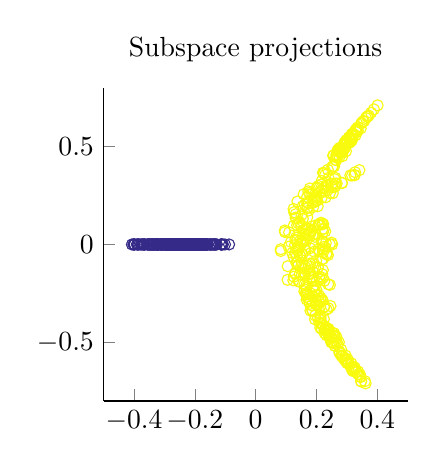
\begin{tikzpicture}

\begin{axis}[%
width=1.520833in,
height=1.565625in,
scale only axis,
colormap={mymap}{[1pt] rgb(0pt)=(0.2081,0.1663,0.5292); rgb(1pt)=(0.211624,0.189781,0.577676); rgb(2pt)=(0.212252,0.213771,0.626971); rgb(3pt)=(0.2081,0.2386,0.677086); rgb(4pt)=(0.195905,0.264457,0.7279); rgb(5pt)=(0.170729,0.291938,0.779248); rgb(6pt)=(0.125271,0.324243,0.830271); rgb(7pt)=(0.0591333,0.359833,0.868333); rgb(8pt)=(0.0116952,0.38751,0.881957); rgb(9pt)=(0.00595714,0.408614,0.882843); rgb(10pt)=(0.0165143,0.4266,0.878633); rgb(11pt)=(0.0328524,0.443043,0.871957); rgb(12pt)=(0.0498143,0.458571,0.864057); rgb(13pt)=(0.0629333,0.47369,0.855438); rgb(14pt)=(0.0722667,0.488667,0.8467); rgb(15pt)=(0.0779429,0.503986,0.838371); rgb(16pt)=(0.0793476,0.520024,0.831181); rgb(17pt)=(0.0749429,0.537543,0.826271); rgb(18pt)=(0.0640571,0.556986,0.823957); rgb(19pt)=(0.0487714,0.577224,0.822829); rgb(20pt)=(0.0343429,0.596581,0.819852); rgb(21pt)=(0.0265,0.6137,0.8135); rgb(22pt)=(0.0238905,0.628662,0.803762); rgb(23pt)=(0.0230905,0.641786,0.791267); rgb(24pt)=(0.0227714,0.653486,0.776757); rgb(25pt)=(0.0266619,0.664195,0.760719); rgb(26pt)=(0.0383714,0.674271,0.743552); rgb(27pt)=(0.0589714,0.683757,0.725386); rgb(28pt)=(0.0843,0.692833,0.706167); rgb(29pt)=(0.113295,0.7015,0.685857); rgb(30pt)=(0.145271,0.709757,0.664629); rgb(31pt)=(0.180133,0.717657,0.642433); rgb(32pt)=(0.217829,0.725043,0.619262); rgb(33pt)=(0.258643,0.731714,0.595429); rgb(34pt)=(0.302171,0.737605,0.571186); rgb(35pt)=(0.348167,0.742433,0.547267); rgb(36pt)=(0.395257,0.7459,0.524443); rgb(37pt)=(0.44201,0.748081,0.503314); rgb(38pt)=(0.487124,0.749062,0.483976); rgb(39pt)=(0.530029,0.749114,0.466114); rgb(40pt)=(0.570857,0.748519,0.44939); rgb(41pt)=(0.609852,0.747314,0.433686); rgb(42pt)=(0.6473,0.7456,0.4188); rgb(43pt)=(0.683419,0.743476,0.404433); rgb(44pt)=(0.71841,0.741133,0.390476); rgb(45pt)=(0.752486,0.7384,0.376814); rgb(46pt)=(0.785843,0.735567,0.363271); rgb(47pt)=(0.818505,0.732733,0.34979); rgb(48pt)=(0.850657,0.7299,0.336029); rgb(49pt)=(0.882433,0.727433,0.3217); rgb(50pt)=(0.913933,0.725786,0.306276); rgb(51pt)=(0.944957,0.726114,0.288643); rgb(52pt)=(0.973895,0.731395,0.266648); rgb(53pt)=(0.993771,0.745457,0.240348); rgb(54pt)=(0.999043,0.765314,0.216414); rgb(55pt)=(0.995533,0.786057,0.196652); rgb(56pt)=(0.988,0.8066,0.179367); rgb(57pt)=(0.978857,0.827143,0.163314); rgb(58pt)=(0.9697,0.848138,0.147452); rgb(59pt)=(0.962586,0.870514,0.1309); rgb(60pt)=(0.958871,0.8949,0.113243); rgb(61pt)=(0.959824,0.921833,0.0948381); rgb(62pt)=(0.9661,0.951443,0.0755333); rgb(63pt)=(0.9763,0.9831,0.0538)},
xmin=-0.5,
xmax=0.5,
ymin=-0.8,
ymax=0.8,
title={Subspace projections},
axis x line*=bottom,
axis y line*=left
]
\addplot[scatter,only marks,scatter src=explicit,scatter/use mapped color={mark=o,mark options={},draw=mapped color}] plot table[row sep=crcr,meta index=2]{%
-0.264653152655549	-3.86261475046704e-12	-1\\
0.131471026053184	0.154191893645676	1\\
0.315281829157397	-0.635588978803027	1\\
-0.226252735659498	2.52281295566177e-13	-1\\
-0.18349880264346	-2.55798285252314e-12	-1\\
0.356908894325939	0.629961850352138	1\\
0.196039781307366	0.0965921636586217	1\\
-0.164121993497827	-1.96968959922657e-12	-1\\
0.315641365512264	0.557260590006791	1\\
-0.136422667772503	2.38358440323981e-13	-1\\
-0.326952345353268	-6.61680476993122e-12	-1\\
0.206170023606679	-0.0250307904977847	1\\
-0.23848990330881	-4.95720560733767e-13	-1\\
0.144931556369965	0.114181157248137	1\\
-0.185526261780386	2.25176901817179e-12	-1\\
-0.180645799995056	1.36940929727951e-12	-1\\
-0.211061967137229	-9.57692178452143e-13	-1\\
0.297718355477342	0.531401459527212	1\\
0.153094367144851	0.0090174150896386	1\\
0.152207770042532	-0.0924735765848014	1\\
-0.130687279117765	-8.20046597769953e-13	-1\\
0.201782721730402	-0.304563693148406	1\\
0.21254091945125	-0.425928304160475	1\\
0.16469226817068	0.0544390781927589	1\\
-0.243154064507279	3.14852168683933e-12	-1\\
0.200752914105754	-0.25913464619237	1\\
0.217236775123426	0.324292681569621	1\\
-0.194182626027705	1.26086396360425e-12	-1\\
-0.369233657336843	-7.44091070721355e-12	-1\\
-0.200275777475127	2.24464893854062e-12	-1\\
-0.366265765588562	-7.41733009029986e-12	-1\\
0.224349416471141	0.0796292818998895	1\\
0.361517566481546	-0.709844266197595	1\\
0.173279452442063	0.271366925138316	1\\
0.244150239944205	0.262291240841096	1\\
-0.397790855461685	8.68089339107651e-12	-1\\
-0.377500430882225	8.23462751856663e-12	-1\\
-0.220272579315862	-9.48101318944929e-13	-1\\
0.331640183193228	0.589800503751546	1\\
0.120522214448801	-0.0432469901491635	1\\
0.284475021337736	0.467877925819794	1\\
0.212757310545326	-0.385043246930282	1\\
-0.270985044597682	-1.21747637768321e-12	-1\\
-0.165499206595992	-2.27144887530178e-12	-1\\
0.160584782003781	-0.147017043484783	1\\
-0.222093079428528	-2.65874902424449e-12	-1\\
0.321961630764261	0.560693691698406	1\\
-0.228095202092168	-6.73197366604232e-13	-1\\
-0.250584807135545	5.08544926987147e-12	-1\\
0.266193510857066	-0.477596291472227	1\\
-0.226252498670554	-3.78792513180176e-12	-1\\
-0.282840964060266	3.14041353115956e-12	-1\\
0.208996306446923	-0.397143810899627	1\\
-0.250109239733047	-3.05689852989826e-12	-1\\
0.368684637758035	0.65384086098624	1\\
0.227368746832153	-0.434212480282504	1\\
-0.177079409686234	-1.94797531915468e-12	-1\\
0.275089791223928	-0.547070471202915	1\\
0.132828300661872	0.0354413694817663	1\\
0.130843991891449	0.0240174538234243	1\\
0.18916332499877	0.1912440711496	1\\
0.277335197180651	0.477673795083825	1\\
-0.311991566298338	-6.31959379921326e-12	-1\\
-0.255179858266636	-4.38787695496035e-12	-1\\
0.178634955634613	0.0525532409	1\\
-0.222826381026454	-3.30894108297237e-12	-1\\
0.160093188411049	-0.239310113526753	1\\
-0.198913634956384	2.86403248732507e-13	-1\\
-0.113577401247162	1.64328919539672e-12	-1\\
0.221081312710671	-0.131003230683843	1\\
0.148652100582401	-0.116541924017777	1\\
-0.295575104275677	-5.93475126227663e-12	-1\\
0.163060734689125	0.0772153690670615	1\\
-0.208924557801221	-1.21263585007123e-12	-1\\
0.126236625523417	0.165037918262652	1\\
0.124681244246223	0.181352067660637	1\\
0.248371517459161	-0.499396500025152	1\\
0.309722754394729	0.536942847680311	1\\
-0.191605288888416	-1.79907712037427e-12	-1\\
-0.266925255230796	4.14186542139384e-12	-1\\
0.147215211174562	-0.0612886566732081	1\\
0.161576955509318	0.204169058354623	1\\
-0.187901531863729	-1.13736136511596e-13	-1\\
-0.312195972794249	6.7453746562255e-12	-1\\
-0.334543152717487	5.26125167257321e-12	-1\\
0.244174591712914	-0.206493746620176	1\\
0.31836313897878	0.555938113674807	1\\
-0.306338929571605	-5.46111975084452e-12	-1\\
-0.194723084500329	-1.94627596671034e-13	-1\\
-0.308096477218545	5.37635600317886e-12	-1\\
-0.27373524728413	4.67293320262239e-12	-1\\
-0.247481543532917	4.25856609978245e-12	-1\\
-0.324795608736046	-5.66871930753069e-12	-1\\
-0.164437021496454	6.27393338259121e-13	-1\\
0.248715531441977	-0.476303008190358	1\\
0.388846166282352	0.690367434646015	1\\
-0.239049441190681	-1.08667218979061e-12	-1\\
-0.248088762983863	3.71066861761746e-12	-1\\
-0.242814851726427	-4.02207914558033e-12	-1\\
0.230296798371899	0.240977094942069	1\\
0.251710892568433	0.396652682442489	1\\
0.219971940313542	-0.284221481369557	1\\
0.259363122903245	0.293456844405635	1\\
-0.259776519002763	-1.32056691567761e-12	-1\\
0.226476235745593	-0.317788094796634	1\\
-0.248901959871501	-3.94483189095723e-12	-1\\
0.15833071078734	0.074735167032311	1\\
0.315414341789396	0.543802192160256	1\\
-0.254417509005487	-3.68829628774866e-12	-1\\
0.16218970286534	-0.23040545251802	1\\
0.161945079914719	-0.113852296550848	1\\
-0.149915864581546	9.18059514309607e-13	-1\\
0.277216948493832	-0.552477541472126	1\\
0.166326004315701	-0.209567213716675	1\\
0.284084445564618	0.313391008034002	1\\
0.187305010835798	-0.219643381367062	1\\
0.31618120549961	-0.637126467960295	1\\
0.253546533372066	0.261878262937361	1\\
-0.287235612981389	-5.74655989927451e-12	-1\\
0.269476946635787	0.481012813544713	1\\
-0.290261491224441	6.09934181570975e-12	-1\\
-0.316621774170719	-5.52587858277324e-12	-1\\
-0.140767195786926	-5.87270435781901e-13	-1\\
0.249911943467695	0.29211378055402	1\\
0.347266777000082	0.619012254391373	1\\
-0.274063949471092	5.8694312050758e-12	-1\\
0.33580054652012	0.59888878722888	1\\
-0.227087516990136	-8.29766578452846e-13	-1\\
0.366488603174719	0.653146863041554	1\\
0.296720655960576	-0.593457902814284	1\\
-0.258231323460114	-4.94421562900217e-12	-1\\
0.125242647021882	0.0961131728600016	1\\
0.302849779082912	0.521627281082642	1\\
0.190092315969315	0.00367140125470285	1\\
0.20874301497432	-0.290355800407256	1\\
-0.246759473297924	-6.97000582867858e-13	-1\\
-0.167349114394371	-8.96492818155322e-13	-1\\
-0.203783185295841	-2.65947885381175e-12	-1\\
0.279104363618135	0.471127097039869	1\\
0.294067969529056	0.493883804278036	1\\
0.169942473341904	0.215016506691933	1\\
0.311985037164968	0.533884045838804	1\\
0.348313341333768	0.619520957101566	1\\
-0.198263121769657	3.30521663889764e-12	-1\\
0.174533380053082	0.173594288123235	1\\
-0.223213825171353	-3.0379024293352e-12	-1\\
-0.258588468067242	-2.93773275495683e-12	-1\\
-0.253644696094114	-1.23570176449072e-12	-1\\
0.302603841646622	-0.58724852578943	1\\
0.169665288505817	0.138894911592893	1\\
-0.231217308762189	-1.58504492388727e-12	-1\\
0.217987580062886	-0.0764940176265112	1\\
-0.293452529816952	-5.83740351443601e-12	-1\\
-0.150470679722923	1.4532821084726e-12	-1\\
-0.262161263028703	-5.24537561316137e-12	-1\\
0.202413367440419	0.224822245509138	1\\
0.299443406359323	0.533361411587776	1\\
-0.294638480617182	5.25440036503362e-12	-1\\
-0.269351167143125	-5.35964055153342e-12	-1\\
-0.232675394446024	5.91906344929693e-13	-1\\
0.125249010351653	-0.164641452103534	1\\
-0.22839947122346	2.51897186829889e-12	-1\\
0.259747528557444	0.333486177722495	1\\
-0.294587035347824	4.70862199350368e-12	-1\\
-0.308061783408717	6.07800519000423e-12	-1\\
0.230599922464825	0.00726519693012122	1\\
0.20049881581692	0.240145795410485	1\\
-0.293084468602577	5.77756023318854e-12	-1\\
0.254705248410952	0.45384127117876	1\\
0.346843790440631	-0.699488728111594	1\\
-0.172361898730553	1.15519636897096e-13	-1\\
0.186762511606418	0.0470302601027557	1\\
0.215007165530867	0.111218824015179	1\\
0.275725448169808	0.447871932885156	1\\
0.246063111545265	-0.314525323628552	1\\
0.232449578731762	-0.44324709789999	1\\
0.221341127400981	0.366467375199554	1\\
0.131367228270229	0.137276489984795	1\\
-0.204042339582649	-2.81200766833322e-12	-1\\
-0.329193913416953	6.46643205770323e-12	-1\\
-0.194106632962796	-2.20656647037408e-12	-1\\
-0.246917868740849	-4.3480820313257e-12	-1\\
0.285079212837328	0.450785274819027	1\\
-0.244459605572386	2.58990213629148e-12	-1\\
-0.295245404459134	-5.13604708618887e-12	-1\\
-0.17127364589039	1.95233641084325e-12	-1\\
0.0826980063206656	-0.0334546951099051	1\\
-0.270218962111518	4.38737266470766e-12	-1\\
0.156066386335045	-0.120028004302546	1\\
-0.263977490201465	4.75428326370118e-12	-1\\
-0.214862064852073	-5.43624695099457e-13	-1\\
0.22955985596898	-0.0175900961291013	1\\
-0.266713523852279	5.6881382320509e-12	-1\\
0.26640395312506	0.311227047159119	1\\
-0.355217914493087	-7.10723182488175e-12	-1\\
0.341108964510968	0.37986623426169	1\\
0.20572748190059	0.0995605366560629	1\\
-0.356212663238052	7.77206602255256e-12	-1\\
0.194126632812611	-0.214297834013163	1\\
0.288887918393972	-0.581351213337792	1\\
-0.238842226229153	4.98222340742795e-12	-1\\
0.136462965058193	0.0982059406223995	1\\
-0.345541786108365	-6.92756367784209e-12	-1\\
0.221568019437802	-0.0401251226861017	1\\
0.19821423903161	-0.30697732198505	1\\
-0.238606529292776	-3.63229590870361e-12	-1\\
0.216799337509977	-0.406249584817545	1\\
0.180175971170056	-0.338282968000331	1\\
0.16089594850845	-0.203749301666393	1\\
-0.304965346974699	-5.26600588894133e-12	-1\\
-0.195495020384408	-2.69193923678964e-12	-1\\
-0.146551279283883	1.43338462123419e-12	-1\\
0.206240284979311	0.298849580813694	1\\
0.254779329377202	0.39924158151523	1\\
-0.242171329257356	3.53875706194765e-12	-1\\
0.212320703681236	-0.402686074328439	1\\
-0.198467676501051	-3.77715965158504e-12	-1\\
0.277348652406366	0.494584530529785	1\\
-0.227207111831532	4.7417968111615e-12	-1\\
0.210422233574959	0.261680090027354	1\\
-0.145825446640862	-1.00492365854994e-12	-1\\
-0.248113598546181	-4.3828907236691e-12	-1\\
-0.253783770734995	4.95245938538597e-12	-1\\
0.188282466482085	0.212338404002942	1\\
-0.296970657341052	3.34954527093327e-12	-1\\
-0.131814931372562	-8.9634658709224e-14	-1\\
0.166728284981568	-0.222675493386613	1\\
-0.228999666886447	-3.39064478699476e-12	-1\\
0.171313355376132	0.0788131667081066	1\\
-0.165411521504333	2.26282957668657e-12	-1\\
-0.222689677838779	-1.13180089644585e-12	-1\\
0.27401300043861	0.476834421243032	1\\
-0.297963158316369	-5.99233120670347e-12	-1\\
0.265256082353219	0.430537770061947	1\\
0.140933234374353	-0.0162727363981472	1\\
0.307363159218874	0.547138158313031	1\\
0.240372040413224	-0.453402457770487	1\\
0.175719801644564	0.263623807882607	1\\
0.320014950129263	-0.624055604513347	1\\
0.218887761375116	0.102741488342566	1\\
0.262946875283395	0.309752840622168	1\\
-0.269245539513919	-1.04317581458328e-12	-1\\
0.269343398470661	-0.507923517149291	1\\
-0.17073503863534	2.5068483414718e-12	-1\\
0.174096659031516	0.208618884795116	1\\
0.178111629223998	0.285946288565744	1\\
-0.399022055311512	-8.07217532430208e-12	-1\\
-0.219385808577721	-2.50541666431888e-12	-1\\
-0.250405343356775	3.86638081667169e-12	-1\\
0.321175507758922	-0.632171842492556	1\\
-0.250921901360081	-1.06176060600199e-12	-1\\
0.226527268720883	-0.452826472251691	1\\
-0.180637533068628	3.35996961884018e-12	-1\\
0.31780906180366	0.542203379094372	1\\
-0.155982245694555	-2.119406705695e-12	-1\\
-0.233858782767796	-3.26886575192697e-12	-1\\
-0.292437697453228	-1.31631349990258e-12	-1\\
-0.246948392008941	5.19173910640484e-12	-1\\
-0.269574349886648	5.71125943096021e-12	-1\\
0.140242471884232	0.107781378353187	1\\
0.218580505273393	0.00270755739554386	1\\
-0.224440046994684	3.68484331024901e-12	-1\\
-0.279958925385857	-3.19646306025002e-12	-1\\
0.18548041322464	-0.166207939605176	1\\
0.233527212972329	-0.332499405704889	1\\
-0.334219748688611	5.12774019847602e-12	-1\\
0.225044056165489	0.363840509544424	1\\
-0.207007857025565	-3.31266571285374e-12	-1\\
-0.232648934723921	-4.46455580280678e-12	-1\\
0.140194050809867	-0.105311674923811	1\\
-0.170946637060789	4.69824124107276e-13	-1\\
0.168376094423486	-0.26705350205293	1\\
-0.285072982522652	4.43002079850001e-12	-1\\
0.169469511612828	0.187520101136014	1\\
-0.187305817128215	5.68100356450375e-13	-1\\
0.345512368487049	0.592654342098415	1\\
-0.241870467580987	3.84655812058757e-12	-1\\
-0.196644585352521	-1.81602030391842e-12	-1\\
0.155194758635059	0.131017267459092	1\\
0.237505057785649	0.381775704494468	1\\
0.186583900806751	-0.0979861790939259	1\\
-0.217091242418246	4.33907501996654e-12	-1\\
-0.189255556887364	4.75115284814157e-13	-1\\
-0.275234269622282	4.34024542129798e-12	-1\\
0.18976911067567	-0.142491794455372	1\\
0.161815832256141	-0.00026925972023794	1\\
-0.295814578428795	-5.16990407804574e-12	-1\\
-0.264430362624081	3.96883384490241e-12	-1\\
0.238627923196082	-0.2034838302903	1\\
-0.26838983292473	-4.61071971309193e-12	-1\\
-0.201650177458427	2.86190929572697e-12	-1\\
-0.245113679398865	-4.83714661272175e-12	-1\\
-0.19931578867818	-3.33795512786088e-12	-1\\
0.151723953948135	0.016353068569158	1\\
0.288675782917529	0.480245573977837	1\\
0.133771199174526	-0.0944393405522026	1\\
0.200337500792637	0.228129764797044	1\\
-0.145233843889098	5.54228302656009e-13	-1\\
-0.364412706113377	-7.34245163668744e-12	-1\\
-0.168378648511282	1.97320731584186e-12	-1\\
-0.264618729797106	4.65066737599401e-12	-1\\
-0.220023307760267	2.69601551748183e-12	-1\\
-0.24186758011411	-7.18509886572175e-13	-1\\
0.237469947547603	-0.433488893911154	1\\
0.359523040378702	-0.698465995725134	1\\
0.221051395041222	-0.171084076577553	1\\
0.20500789613797	-0.117147908809185	1\\
-0.217633318496176	-1.04937942816256e-12	-1\\
-0.267736126881849	4.48866372034479e-12	-1\\
-0.365634497337768	7.97850902298843e-12	-1\\
-0.243001523331944	-1.19982665500818e-12	-1\\
-0.291550058125992	-5.14697118236131e-12	-1\\
-0.199930183899263	-1.26003529877562e-12	-1\\
0.252247734134143	-0.500242120077993	1\\
0.269912605602685	0.481486924623814	1\\
-0.367416806033813	-7.38026493999141e-12	-1\\
-0.341776673906478	-6.91157369846092e-12	-1\\
0.307073685011734	0.546871464637251	1\\
-0.230404694651199	-4.45892810785524e-12	-1\\
-0.236416394011057	5.07178479778951e-12	-1\\
-0.25255025031377	5.45281288953458e-12	-1\\
0.146766498460885	0.0197970232372291	1\\
-0.186304609653374	3.36181620794876e-12	-1\\
-0.325343118361774	4.97249750421898e-12	-1\\
-0.223836672432032	4.87142046583137e-12	-1\\
-0.194814554755965	3.22460331134626e-12	-1\\
0.281261105388943	-0.537028059661129	1\\
0.281534405727504	-0.567642713325286	1\\
0.258122359371502	0.399024360932769	1\\
-0.177681845176078	-1.48092103028296e-14	-1\\
0.177897804311868	-0.303066024937165	1\\
0.21260976333479	-0.367773704315324	1\\
0.198487466202433	0.249222228446472	1\\
-0.309047207310478	6.64461507780978e-12	-1\\
-0.195585905282338	-2.45757781204741e-12	-1\\
-0.242981371757207	3.73987726303638e-12	-1\\
-0.210038914841156	-2.06541602185447e-13	-1\\
0.185351293085358	-0.184419768216129	1\\
0.10505722918709	-0.180839837580464	1\\
0.164105661846112	-0.0319724799320948	1\\
0.237814521294972	-0.0545573366338929	1\\
-0.198381475762192	2.53430545080745e-12	-1\\
-0.274121883434626	-4.9300356594604e-12	-1\\
0.262217742368104	0.340451122718574	1\\
-0.218838425373479	3.57866040322191e-12	-1\\
0.362516681259827	0.645932297349705	1\\
-0.284906102612633	6.0771231292166e-12	-1\\
-0.265966778892539	4.90837319235617e-12	-1\\
0.291415857629164	0.518914443883752	1\\
0.185996868481186	-0.172130683020137	1\\
0.181305466822995	-0.0606710387574499	1\\
-0.28872892054159	-4.9388662886597e-12	-1\\
-0.355446014400843	-7.17022976319454e-12	-1\\
-0.239780523091321	-5.15570367989958e-13	-1\\
0.308555083565002	0.539019324895473	1\\
-0.227135424630331	-3.32726941462749e-12	-1\\
-0.11405096311401	1.23045964001791e-12	-1\\
-0.234414781973368	2.98088883882746e-12	-1\\
-0.293435640492074	5.8438720657131e-12	-1\\
-0.180569836915257	1.83080998343449e-12	-1\\
-0.107731285996113	-1.41678540478546e-12	-1\\
0.301115940139244	0.525059822261752	1\\
-0.241995065959674	4.21446525367574e-12	-1\\
-0.401405823502327	8.76324409502417e-12	-1\\
0.226431248055596	-0.439246596951164	1\\
0.28373432971462	-0.571735825780782	1\\
-0.201422361530833	2.66012047584061e-12	-1\\
0.250704401825887	-0.498006355635157	1\\
0.186238613166801	0.257918332252681	1\\
-0.214139268550001	3.17246159239847e-12	-1\\
-0.215037392124716	3.73484855397657e-13	-1\\
-0.167705439605213	5.25663959678897e-13	-1\\
-0.240834248798796	-4.71747683023539e-12	-1\\
0.312056456618772	0.538959280126254	1\\
0.179752550262684	-0.149132787147407	1\\
-0.258759026790622	-4.92358441173109e-12	-1\\
-0.222387841430961	-4.00002150040585e-12	-1\\
-0.217238902206504	1.9060463042855e-12	-1\\
-0.20310032984322	1.93841656812548e-12	-1\\
0.271889839967347	0.473475438643215	1\\
0.221592014573788	-0.0736483400945823	1\\
0.21675481057123	0.237620615822616	1\\
-0.349608468107015	6.90675413943768e-12	-1\\
-0.278585310503959	5.95924599961963e-12	-1\\
0.237853102384457	-0.457288637131729	1\\
0.26410984564508	-0.469788275989265	1\\
0.199716859641355	-0.231803543545777	1\\
-0.349354680767269	-7.04162299002589e-12	-1\\
-0.277924159429895	6.0471361244535e-12	-1\\
-0.344624320202087	7.50150922493115e-12	-1\\
0.251213386042519	-0.477744226238884	1\\
-0.202827927707141	3.70350787033001e-12	-1\\
0.344012930779282	-0.674639731246299	1\\
0.0966012997997304	0.0635036717165008	1\\
0.295477225056469	-0.594903287239301	1\\
0.150441054953508	0.0882727572750783	1\\
0.22215940083787	0.104522186494814	1\\
-0.268374664064055	5.6112832709822e-12	-1\\
0.195808004783758	-0.116800676049363	1\\
-0.189084327974076	-3.6205779946876e-12	-1\\
0.204887891532199	-0.117196137051797	1\\
0.141795224411003	-0.189684295971687	1\\
-0.198385044057055	-3.67124758182266e-12	-1\\
-0.188272759525972	-9.7231091463535e-13	-1\\
0.295956569630048	-0.567732851549403	1\\
0.266878614850647	0.459562476946249	1\\
-0.134174017348015	2.64422081139245e-12	-1\\
0.314500430096875	-0.606930921822247	1\\
0.196882034520118	-0.283041730964016	1\\
-0.199821801569325	-2.59637276723432e-12	-1\\
-0.244599547238809	-4.39923306698521e-12	-1\\
0.174476542445561	0.0605213431991292	1\\
-0.288045037208494	3.28677889674184e-12	-1\\
-0.197817106582968	-1.39078944303024e-12	-1\\
-0.277899144140838	-1.29913507876548e-12	-1\\
-0.205380238398391	3.63093123135992e-12	-1\\
0.325365929453312	0.354998175651802	1\\
-0.110677169602983	9.55418413002157e-14	-1\\
0.154615901666714	0.195036213225944	1\\
-0.258309973582286	-3.04617008244384e-12	-1\\
-0.240439085088912	4.34342109317556e-12	-1\\
0.218727757912702	-0.151671442635084	1\\
0.217317977517029	0.27708310818934	1\\
-0.247606849644961	3.39097328701326e-12	-1\\
-0.254398998039419	-1.37277963840928e-12	-1\\
-0.160830809700894	-7.88073890932102e-13	-1\\
0.241309508573026	-0.466495421996541	1\\
0.32693230513932	-0.644518841239135	1\\
0.325910001204371	-0.630422842063127	1\\
-0.20058580895028	-3.88120528429604e-12	-1\\
-0.245268923121042	4.19607631164925e-12	-1\\
-0.310762074039361	6.70021983897984e-12	-1\\
-0.160790576841755	1.19766381472988e-12	-1\\
0.233547523660687	-0.435884256703004	1\\
-0.334241263990887	-6.67233239742277e-12	-1\\
-0.264178550736658	-1.28806108580634e-12	-1\\
-0.263519405766311	4.07119635526041e-12	-1\\
0.230892134749672	-0.42360099997303	1\\
-0.234466797186174	-3.71002847084149e-12	-1\\
0.144656901890432	-0.189187774723954	1\\
-0.167098102430456	1.94585046921208e-12	-1\\
0.21150295624995	-0.176423656526236	1\\
-0.269661038326549	-4.39594251161388e-12	-1\\
-0.301208730452269	6.53305212046708e-12	-1\\
-0.261977317533784	-5.03002205604974e-12	-1\\
-0.282824049888775	-4.53595466643177e-12	-1\\
0.290986387170291	0.507635484774086	1\\
-0.232106449374172	3.81152101880618e-12	-1\\
-0.284753184316942	-4.78408084020049e-12	-1\\
-0.191064337390892	-1.36432636259726e-12	-1\\
-0.322444823898976	5.13586621053486e-12	-1\\
-0.187476072114216	-1.19694714321171e-12	-1\\
-0.238271143948903	4.86269535535427e-12	-1\\
0.192745111215739	-0.235857963340979	1\\
0.199048049021535	-0.0827980831793612	1\\
0.167690514000029	0.0252796285745254	1\\
0.219069318913452	0.0778949619216727	1\\
0.342721281082577	-0.663933477805722	1\\
-0.250968433820332	3.75366102553063e-12	-1\\
0.336714219297491	-0.662762716869206	1\\
0.328433596920007	0.557542226820183	1\\
-0.310641027200104	4.91297343462576e-12	-1\\
-0.204663490582137	-9.38886649033373e-13	-1\\
0.183121604259183	-0.16814247028129	1\\
-0.186126308458462	-7.68202393638859e-14	-1\\
-0.257754629660084	4.04965202982384e-12	-1\\
0.332356220440569	0.574047508637376	1\\
0.325495000396322	0.353929738773022	1\\
0.178859548968723	0.256086798713031	1\\
-0.246444410476494	5.17262809661082e-12	-1\\
0.26065710376128	-0.518265346559248	1\\
0.267175174028354	0.444777524922773	1\\
-0.174965513437833	-2.27975325040941e-12	-1\\
0.309071600282522	0.519636658531241	1\\
-0.1964906109648	2.49790067528878e-12	-1\\
0.208882543061064	-0.165015549501421	1\\
0.136750560436379	0.0221569568828193	1\\
0.174049783917704	-0.27575364736352	1\\
0.137318659784786	0.219411318846738	1\\
-0.350973313924578	-7.09066011505909e-12	-1\\
0.132755656894663	0.133124871072888	1\\
0.299591104467687	0.512279860861265	1\\
0.212389676203056	-0.315362458526027	1\\
-0.216034112558152	-3.71106883553593e-12	-1\\
-0.319311966019601	-5.24823904276087e-12	-1\\
-0.385917460452605	8.42784337852931e-12	-1\\
-0.18342304259266	-2.69152190743712e-12	-1\\
0.178945521769698	-0.0973910679851034	1\\
-0.247496803959271	4.85897499806854e-12	-1\\
0.243750323797844	0.00072380183078823	1\\
0.206595989518681	0.0984885630589096	1\\
-0.300788662230982	6.55504817451144e-12	-1\\
-0.241647111104039	-4.2814828449962e-12	-1\\
0.20410134232567	0.195043531685394	1\\
-0.265286907676746	-4.85619431355927e-12	-1\\
0.205147887636444	-0.374197362068495	1\\
-0.215232653106604	2.3427147614101e-12	-1\\
0.194491401800341	0.253935992210751	1\\
0.214222969754967	-0.273299970030416	1\\
-0.19214188701336	3.58068498093641e-12	-1\\
0.145137098409723	-0.0536514543900627	1\\
-0.137422619870239	2.11801436815732e-12	-1\\
0.179404576258773	-0.0192502206678598	1\\
0.283210291209192	0.315225289794425	1\\
-0.192251691581474	-5.8879903147968e-13	-1\\
-0.268481885745908	-4.65184725998732e-12	-1\\
0.298833942827347	0.521323987395035	1\\
0.296972200695986	0.47609215351249	1\\
0.166542415715801	-0.247520420515562	1\\
0.275892401027171	-0.555315435600765	1\\
-0.269129759091139	4.81838105709398e-12	-1\\
-0.12747091068736	-1.44629128511557e-12	-1\\
-0.231028457667595	4.59066872954441e-12	-1\\
-0.319779180479129	6.27088167688597e-12	-1\\
-0.258566120626835	5.59571798487808e-12	-1\\
-0.178430202637881	1.8656055559875e-12	-1\\
0.171731104230474	0.186439898077997	1\\
-0.265511253774801	3.96937245949173e-12	-1\\
-0.216440387790031	-1.70756710822926e-12	-1\\
0.316914167502165	0.352178762741138	1\\
0.224333466768209	-0.318784206156664	1\\
-0.198128785599969	-2.77205976097866e-12	-1\\
-0.163026868383604	2.0039965333333e-13	-1\\
-0.325224324600265	5.07414063101277e-12	-1\\
0.151565848290056	-0.155096178368498	1\\
0.220494910448159	0.0140809839099473	1\\
0.251538535162442	-0.000100695975423154	1\\
0.148494547661783	0.00408160004583486	1\\
0.315894941005708	0.563610013620447	1\\
0.257979240743954	-0.464454102492239	1\\
0.201604501204651	-0.304844000173222	1\\
0.0825093184433783	-0.0243683162016038	1\\
0.185632542321312	-0.334448625152491	1\\
0.319975642946943	-0.645318359216841	1\\
-0.286761038014183	4.59385988209607e-12	-1\\
-0.205186273945896	3.31984828214236e-12	-1\\
-0.228245325221371	3.35087732479843e-12	-1\\
0.22740241037149	0.270687621536914	1\\
0.16934054792664	0.243242626786467	1\\
-0.382024417060459	-7.72878560634702e-12	-1\\
-0.294703669963214	6.3339947308219e-12	-1\\
-0.176859362765351	4.16295831304776e-13	-1\\
0.265957381817167	0.461349218441885	1\\
0.217731482233016	0.0180707465132179	1\\
0.207997405928823	-0.290943801219647	1\\
-0.227334499427789	4.72522800535222e-12	-1\\
-0.275794686464589	5.87380199301707e-12	-1\\
0.33674966060612	-0.648191277349056	1\\
-0.148848004929239	5.83322944251194e-13	-1\\
0.181411445950174	-0.250531954849465	1\\
-0.277421167748355	-4.80024110777532e-12	-1\\
0.153709853512078	-0.0500023010488169	1\\
0.237087244556655	0.278250259417218	1\\
0.301087636705669	-0.606969551424636	1\\
-0.246434624842315	-4.56905786105869e-12	-1\\
0.273620186836704	-0.499702835628527	1\\
-0.288845023310173	-4.84230995344656e-12	-1\\
0.220644951165393	-0.0252133586875415	1\\
0.213591947935211	-0.374956225516277	1\\
-0.308405381076515	5.36336352889546e-12	-1\\
0.157988959966319	0.256599302815888	1\\
-0.25052298229169	2.87257933772529e-13	-1\\
0.208978974655677	-0.0334610177351812	1\\
0.224635391666468	0.287171669431529	1\\
-0.309451041099038	4.93650668425284e-12	-1\\
-0.264653285426512	5.73790427969983e-12	-1\\
-0.306952898054855	4.72991889636763e-12	-1\\
-0.277468406371012	6.00431700202514e-12	-1\\
0.305821059277772	-0.605135313021879	1\\
0.261374380076129	0.432721584842971	1\\
0.130026284663228	-0.146549359642174	1\\
0.327233053683284	0.369037476258574	1\\
0.319111100017841	0.567169143490333	1\\
-0.245357680857765	-3.54388693236402e-12	-1\\
0.0957578878844223	0.0712207862122355	1\\
-0.372685620409904	-7.54715419257073e-12	-1\\
-0.230203855169283	-1.1528192835001e-12	-1\\
-0.328969849838708	-5.68634316394121e-12	-1\\
-0.257053917919124	-3.52741448549125e-12	-1\\
0.223677380131698	-0.415300096309847	1\\
0.295652838231046	-0.583018005150869	1\\
-0.236310161056017	-4.09057351434532e-12	-1\\
-0.280684095719591	-4.86246551826185e-12	-1\\
-0.267245406274135	-4.79864125920515e-12	-1\\
0.19510810556244	-0.38240900570437	1\\
0.249739609272116	0.00918482422053598	1\\
-0.261036671227489	2.78147360735539e-12	-1\\
-0.233938449341085	-3.53355326228965e-12	-1\\
-0.234153924682906	-1.70973434412058e-12	-1\\
0.240115060089445	-0.431561385711949	1\\
-0.287189144859594	-5.05300404051534e-12	-1\\
-0.221468172089698	-3.64786000021789e-12	-1\\
0.257103694430314	0.45600438561995	1\\
0.223953150234885	0.364568643204141	1\\
0.225898266722298	-0.185896012929035	1\\
-0.234872334496735	4.93703401701685e-12	-1\\
-0.388059967338478	-7.84468566119392e-12	-1\\
0.105301637046146	-0.111223562674449	1\\
-0.365782334722942	7.98688234122417e-12	-1\\
-0.22673236227649	4.8667218575499e-12	-1\\
0.197008605819909	0.221177789427765	1\\
0.260646634357478	-0.493257305629851	1\\
-0.241625649428757	4.69023286376016e-12	-1\\
0.311374306413898	0.35308481520857	1\\
-0.182115583866061	6.04721491200246e-13	-1\\
0.134893034604919	-0.0598813548339737	1\\
0.139383826824564	-0.0321584498556203	1\\
0.176182294143471	-0.291550752197387	1\\
0.330955445705198	0.582703907784335	1\\
0.345084375303512	-0.677989856888508	1\\
0.176727739438903	-0.133543970950694	1\\
0.125124398289883	-0.0637264852896059	1\\
-0.247654735935051	-1.00990816130745e-12	-1\\
-0.138814948922583	8.93004944333232e-13	-1\\
-0.233560656415561	1.78031058618506e-13	-1\\
-0.193944826350806	-1.06848304721674e-12	-1\\
0.116160535638947	0.0128018438032655	1\\
-0.233949620907519	-3.75421836049947e-12	-1\\
-0.342516255306434	-6.83282163064811e-12	-1\\
0.155393357778941	0.0462879162250852	1\\
0.269649823374761	0.448775263901303	1\\
-0.307870408954439	-6.23343452639256e-12	-1\\
-0.163940464885431	-3.6723551373262e-13	-1\\
0.195596797114274	-0.238799019588708	1\\
-0.224878230905145	-4.28573096950072e-12	-1\\
-0.321698083225029	6.35492636256114e-12	-1\\
-0.289197581033248	5.75904788949329e-12	-1\\
-0.257056395017167	-4.57535770140274e-12	-1\\
0.31516197598502	0.539883015454848	1\\
0.2736553743944	0.479816822538976	1\\
0.239199933767172	-0.325477341305506	1\\
0.240855415903139	-0.442214638717272	1\\
-0.294863879589535	-4.87913538495157e-12	-1\\
0.237331343189312	-0.432848211699736	1\\
-0.287679781468	5.71241089236442e-12	-1\\
0.237227401572356	0.298656927700411	1\\
-0.25288661380454	-1.61539983688957e-12	-1\\
-0.250035200284832	-4.64255570197813e-12	-1\\
-0.281505985197683	-1.40626207875985e-12	-1\\
-0.285505873235077	-5.00952695470139e-12	-1\\
-0.26716999948498	5.61895478920564e-12	-1\\
0.129735619671711	-0.00232516216679338	1\\
-0.100857065960933	1.16466697583608e-13	-1\\
-0.215320575299787	1.44818107050471e-12	-1\\
0.234855592290694	-0.0467168085394575	1\\
0.353058484865522	0.62948145626445	1\\
-0.162817108437625	-2.69348145281059e-12	-1\\
0.183877116096016	-0.310805356784799	1\\
-0.217010100308524	-6.54873640158119e-13	-1\\
0.335869959293059	0.581615640649769	1\\
0.239632123074988	0.340577642384127	1\\
0.17052942543199	-0.250684655865681	1\\
0.217082858681615	-0.430822454645363	1\\
-0.211304923789894	-2.94913983444662e-12	-1\\
-0.112591719394422	4.94147708529099e-13	-1\\
0.379580739932535	0.672827128971548	1\\
-0.284147770860454	-7.97775052285982e-13	-1\\
0.228721919664868	0.0669497702801247	1\\
-0.185586633872853	2.31550598210409e-12	-1\\
-0.232638023482356	-4.13482779504624e-12	-1\\
-0.406783104726142	8.88244815298399e-12	-1\\
-0.336505978716754	-6.76797864043849e-12	-1\\
0.259946687948733	-0.517135229008017	1\\
-0.338707282902842	-6.82893149189416e-12	-1\\
0.173582968039546	0.0438680660616781	1\\
-0.386923170234498	-7.82251137561547e-12	-1\\
0.218135529969524	-0.407524828249145	1\\
-0.319407782777289	-5.40150091087539e-12	-1\\
-0.158734000164231	2.60376976547847e-13	-1\\
0.321230414363685	-0.647737831511895	1\\
0.22114000251626	0.063093115523405	1\\
0.137847096116735	-0.0883148961556188	1\\
0.37166050361877	0.658957731428583	1\\
-0.164514355917912	2.22926723106368e-12	-1\\
0.181392658372127	0.0630676991702115	1\\
-0.257124380892543	4.73592396790128e-12	-1\\
-0.220610830435687	2.63159274112085e-12	-1\\
0.20949346502709	0.101460350697144	1\\
-0.247098844632822	-4.88632511707134e-12	-1\\
0.346856655203588	-0.699470908978337	1\\
0.201812310040978	0.287171140675633	1\\
0.262704233638648	0.298901459036467	1\\
-0.322038211307055	-6.51352918734928e-12	-1\\
0.161463426176352	-0.156684846378754	1\\
0.167598862324058	-0.281448704298208	1\\
-0.205647281120324	4.11011225408543e-12	-1\\
0.316140257248596	0.531215112989738	1\\
0.331490250568325	-0.648853253005313	1\\
-0.23252748056201	-4.25220167700999e-12	-1\\
-0.210657313790352	-3.54405455616749e-12	-1\\
-0.237096283323638	4.66359582519555e-12	-1\\
0.286893238294714	-0.57172758688851	1\\
-0.20888280852036	-1.89260120860391e-12	-1\\
0.190320419550494	-0.269296279601452	1\\
-0.220854819195899	-2.80852455365576e-12	-1\\
0.173436450632064	-0.152515110405908	1\\
0.180670604343611	0.0701323787431061	1\\
0.201284810064608	-0.186736730467212	1\\
0.175417139999648	0.0800596471791695	1\\
0.265526589520447	0.454852844828172	1\\
0.295411909661256	0.525818860601472	1\\
0.312328161992331	0.525920978841716	1\\
-0.0872940935421724	7.8110335485276e-13	-1\\
0.219489324443038	-0.286478671305749	1\\
-0.246798588429619	-4.3019853864022e-12	-1\\
0.197159436550556	0.0529000789996148	1\\
-0.161633558322957	1.25510099408898e-12	-1\\
-0.199268019771198	3.66830000123572e-12	-1\\
0.214902228221742	-0.288455013408014	1\\
-0.390550413665553	8.52774782615912e-12	-1\\
0.200942868417586	0.291703725052171	1\\
0.26394064476413	-0.503946962541583	1\\
-0.207964853671911	3.80467591226366e-12	-1\\
0.19211409125821	0.231072226292633	1\\
-0.323344678263558	-6.54917748964014e-12	-1\\
0.11004613273709	0.0617519921956948	1\\
0.195733724456993	-0.363298351896318	1\\
0.325246337224445	-0.628501145457233	1\\
-0.306159632134195	-6.1970804004592e-12	-1\\
-0.200266673090031	-3.22377012640956e-12	-1\\
0.318985435735443	0.559153090308073	1\\
-0.231939617823787	4.93115818526168e-12	-1\\
-0.26683031731441	-4.45856628656353e-12	-1\\
0.123980466099784	-0.183403141420561	1\\
-0.341478777801451	7.44861354521443e-12	-1\\
-0.213585717330298	1.71308099408261e-12	-1\\
-0.219621413720612	-9.40293232140119e-13	-1\\
-0.255571987648492	4.05769488400056e-12	-1\\
0.192675333191365	-0.0368042262424493	1\\
0.210777178580924	0.101369935964043	1\\
0.232185248344306	-0.0496461328133308	1\\
-0.206883835669052	-3.93277101802199e-12	-1\\
-0.247471768330954	-2.73467353161595e-12	-1\\
0.187990684284688	-0.340110967365478	1\\
0.215715293537257	0.306768912442286	1\\
0.194440657910692	0.0392282331890665	1\\
0.330980961577306	0.584382703133465	1\\
-0.216176618090208	3.41623729988516e-12	-1\\
0.294263670888172	-0.591746184293725	1\\
0.228843462600399	0.355183427901683	1\\
-0.401132333111229	8.75591247223892e-12	-1\\
-0.348535268843436	-7.05939531887885e-12	-1\\
0.197588652162538	-0.287019775975761	1\\
0.257996074010077	-0.453542345662323	1\\
-0.199061622379831	-2.40320558956735e-12	-1\\
-0.286095016706211	-9.43606045848604e-13	-1\\
0.224233732145127	-0.0122465573172671	1\\
-0.220124244676828	-1.55518517512266e-12	-1\\
-0.37457644207751	-7.53749118880486e-12	-1\\
0.129998723114604	-0.150641662662139	1\\
-0.236743352017304	-2.67548747480169e-12	-1\\
-0.333672947315519	-6.64196182753045e-12	-1\\
0.400962917068853	0.710804099792799	1\\
0.13617626903499	-0.0177383604155289	1\\
0.108271927764554	-0.0118062947077152	1\\
0.300804525429606	-0.600701875207302	1\\
-0.213753644816136	-3.16536519861391e-12	-1\\
-0.202093846447246	3.17400569934192e-12	-1\\
0.232260513310569	0.302103396190971	1\\
0.232930660398396	-0.464507805958039	1\\
0.250710951173516	0.31045277951272	1\\
-0.158008224546893	2.10452060106458e-12	-1\\
-0.21143885786511	3.0560494028617e-12	-1\\
-0.232554808690113	-4.1343994914992e-12	-1\\
0.211747771703648	0.102510550680886	1\\
-0.160076229326279	1.15220053931251e-12	-1\\
-0.263199285460299	4.27798715915657e-12	-1\\
0.129803895998856	-0.0408110543685404	1\\
0.259252267330751	-0.470442281589291	1\\
-0.287139757664317	-1.35571707359937e-12	-1\\
-0.285003509262869	4.7820018688578e-12	-1\\
0.292829658288442	0.506628228870982	1\\
0.167386077230092	-0.25457786253991	1\\
-0.172317037073206	1.3391625873289e-12	-1\\
0.327505716949202	0.583679749223734	1\\
0.144765883426591	-0.152354552767487	1\\
0.285043261979749	0.485107357838627	1\\
-0.206196397754726	-2.97967830538502e-12	-1\\
0.274523240166828	0.489915110027333	1\\
-0.191565260870801	3.40554489337685e-12	-1\\
-0.193369467701383	3.82878632603087e-12	-1\\
-0.236337400875611	-4.63276679254726e-12	-1\\
0.253081388002615	-0.452316368109137	1\\
-0.219077562633727	2.45690510233591e-12	-1\\
0.254977733509052	-0.503801725195125	1\\
-0.18302872773949	2.11407742235534e-12	-1\\
-0.399585738181538	8.72219158612807e-12	-1\\
-0.294891408507433	-5.81606261341491e-12	-1\\
0.224346525459232	-0.380935825266737	1\\
-0.282889026957467	5.99166596143411e-12	-1\\
-0.338073580015076	-6.82859034793428e-12	-1\\
-0.204109203115156	4.01823462489962e-12	-1\\
0.284210282560973	0.47951961701036	1\\
-0.304468148132544	-6.1492403693847e-12	-1\\
-0.214227509575457	-1.8121536858917e-12	-1\\
0.150899157267826	0.150694189566414	1\\
0.208059763947628	-0.259927326098952	1\\
0.243978252571756	-0.478350266364074	1\\
-0.238459325596042	-3.67414010443555e-12	-1\\
0.295645837975224	0.507851772939238	1\\
};
\end{axis}
\end{tikzpicture}%
\end{document}
\caption{Spectral clustering and subspace projections using $\sigma^2 = 0.001$.}
% This file was created by matlab2tikz.
% Minimal pgfplots version: 1.3
%
%The latest updates can be retrieved from
%  http://www.mathworks.com/matlabcentral/fileexchange/22022-matlab2tikz
%where you can also make suggestions and rate matlab2tikz.
%
\documentclass[tikz]{standalone}
\usepackage{pgfplots}
\usepackage{grffile}
\pgfplotsset{compat=newest}
\usetikzlibrary{plotmarks}
\usepackage{amsmath}

\begin{document}
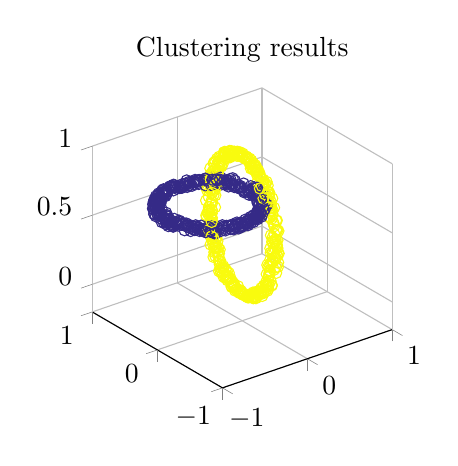
\begin{tikzpicture}

\begin{axis}[%
width=1.5in,
height=1.5in,
scale only axis,
colormap={mymap}{[1pt] rgb(0pt)=(0.2081,0.1663,0.5292); rgb(1pt)=(0.211624,0.189781,0.577676); rgb(2pt)=(0.212252,0.213771,0.626971); rgb(3pt)=(0.2081,0.2386,0.677086); rgb(4pt)=(0.195905,0.264457,0.7279); rgb(5pt)=(0.170729,0.291938,0.779248); rgb(6pt)=(0.125271,0.324243,0.830271); rgb(7pt)=(0.0591333,0.359833,0.868333); rgb(8pt)=(0.0116952,0.38751,0.881957); rgb(9pt)=(0.00595714,0.408614,0.882843); rgb(10pt)=(0.0165143,0.4266,0.878633); rgb(11pt)=(0.0328524,0.443043,0.871957); rgb(12pt)=(0.0498143,0.458571,0.864057); rgb(13pt)=(0.0629333,0.47369,0.855438); rgb(14pt)=(0.0722667,0.488667,0.8467); rgb(15pt)=(0.0779429,0.503986,0.838371); rgb(16pt)=(0.0793476,0.520024,0.831181); rgb(17pt)=(0.0749429,0.537543,0.826271); rgb(18pt)=(0.0640571,0.556986,0.823957); rgb(19pt)=(0.0487714,0.577224,0.822829); rgb(20pt)=(0.0343429,0.596581,0.819852); rgb(21pt)=(0.0265,0.6137,0.8135); rgb(22pt)=(0.0238905,0.628662,0.803762); rgb(23pt)=(0.0230905,0.641786,0.791267); rgb(24pt)=(0.0227714,0.653486,0.776757); rgb(25pt)=(0.0266619,0.664195,0.760719); rgb(26pt)=(0.0383714,0.674271,0.743552); rgb(27pt)=(0.0589714,0.683757,0.725386); rgb(28pt)=(0.0843,0.692833,0.706167); rgb(29pt)=(0.113295,0.7015,0.685857); rgb(30pt)=(0.145271,0.709757,0.664629); rgb(31pt)=(0.180133,0.717657,0.642433); rgb(32pt)=(0.217829,0.725043,0.619262); rgb(33pt)=(0.258643,0.731714,0.595429); rgb(34pt)=(0.302171,0.737605,0.571186); rgb(35pt)=(0.348167,0.742433,0.547267); rgb(36pt)=(0.395257,0.7459,0.524443); rgb(37pt)=(0.44201,0.748081,0.503314); rgb(38pt)=(0.487124,0.749062,0.483976); rgb(39pt)=(0.530029,0.749114,0.466114); rgb(40pt)=(0.570857,0.748519,0.44939); rgb(41pt)=(0.609852,0.747314,0.433686); rgb(42pt)=(0.6473,0.7456,0.4188); rgb(43pt)=(0.683419,0.743476,0.404433); rgb(44pt)=(0.71841,0.741133,0.390476); rgb(45pt)=(0.752486,0.7384,0.376814); rgb(46pt)=(0.785843,0.735567,0.363271); rgb(47pt)=(0.818505,0.732733,0.34979); rgb(48pt)=(0.850657,0.7299,0.336029); rgb(49pt)=(0.882433,0.727433,0.3217); rgb(50pt)=(0.913933,0.725786,0.306276); rgb(51pt)=(0.944957,0.726114,0.288643); rgb(52pt)=(0.973895,0.731395,0.266648); rgb(53pt)=(0.993771,0.745457,0.240348); rgb(54pt)=(0.999043,0.765314,0.216414); rgb(55pt)=(0.995533,0.786057,0.196652); rgb(56pt)=(0.988,0.8066,0.179367); rgb(57pt)=(0.978857,0.827143,0.163314); rgb(58pt)=(0.9697,0.848138,0.147452); rgb(59pt)=(0.962586,0.870514,0.1309); rgb(60pt)=(0.958871,0.8949,0.113243); rgb(61pt)=(0.959824,0.921833,0.0948381); rgb(62pt)=(0.9661,0.951443,0.0755333); rgb(63pt)=(0.9763,0.9831,0.0538)},
xmin=-1,
xmax=1,
tick align=outside,
xmajorgrids,
ymin=-1,
ymax=1,
ymajorgrids,
zmin=-0.2,
zmax=1,
zmajorgrids,
view={-37.5}{30},
title={Clustering results},
axis x line*=bottom,
axis y line*=left,
axis z line*=left
]
\addplot3[scatter,only marks,scatter src=explicit,scatter/use mapped color={mark=o,mark options={},draw=mapped color}] plot table[row sep=crcr,meta index=3]{%
0.449996039057375	0.480325925036146	0.484539559893314	-1\\
0.444026554342783	0.304297700210832	0.511956556253337	-1\\
-0.00579243384541788	-0.548233802576328	0.534048594299953	1\\
-0.0151428744418778	-0.221112117741357	0.958821033891795	1\\
-0.0138089351619959	0.11386309495987	0.97294919017985	1\\
0.00656072303117057	0.436727738701295	0.705351163030866	1\\
0.0244927798244964	0.310538554617753	0.917173235892571	1\\
-0.334360181760132	0.163964366305717	0.479564514119899	-1\\
0.458418209396981	0.209829899364053	0.478478354325021	-1\\
-0.424841381902409	0.722057824636885	0.510828844183328	-1\\
-0.253856121332303	0.0569121253294356	0.501203023350599	-1\\
0.0247121269078962	0.524192071050271	0.63574591403326	1\\
0.0109182339146773	-0.445672725689822	0.489206877035014	1\\
0.0220767127075811	0.535886058588978	0.453691021498569	1\\
0.00572371956704	0.14469382369827	0.98084318501102	1\\
-0.0202857038513214	-0.237014599434988	0.0326239357529515	1\\
-0.0141216104998871	0.453732836162598	0.546560412966627	1\\
-0.00822477793492223	0.403296588845152	0.159062527724841	1\\
0.0049145543606787	0.432231371614402	0.660675560601987	1\\
-0.101086658930327	0.00819117420265325	0.517788108515566	-1\\
0.0218847908027715	-0.152017967648637	0.0131644294560097	1\\
0.0283369937197632	-0.00194295382000684	0.498116776584414	-1\\
-0.111481367490334	0.0181164378379434	0.5083364499603	-1\\
-0.290291558022365	0.907773909633709	0.51993840885386	-1\\
0.277443195465818	0.913421838864534	0.50848824784811	-1\\
0.422702886149167	0.206908184125364	0.478047112116748	-1\\
-0.0211248003194081	0.326714756067945	0.151496391749615	1\\
0.4828611534862	0.66879110828708	0.484236404092475	-1\\
-0.00543710439327398	0.0282694639883208	0.00275639047190547	1\\
-0.0140798911840784	0.493440048319496	0.491040924132826	1\\
-0.381109155511121	0.152980625811269	0.497224867641127	-1\\
0.0210100038552256	0.348999767701628	0.815049966302943	1\\
0.00776252463242632	0.374975974189633	0.840936788356882	1\\
0.42338467463001	0.784216791401532	0.50990771141677	-1\\
0.0175471113349365	0.481852299581482	0.520410920557043	1\\
-0.521083119491365	0.496241649709949	0.503034943131919	-1\\
-0.015798295062685	0.388852783992595	0.249065291329362	1\\
-0.491131835359482	0.656780028015917	0.48952209628946	-1\\
-0.0218267121803668	0.0515655621978446	0.995273024622334	1\\
0.012599143096977	-0.0702122043381784	0.983215411741604	1\\
-0.0116384814533579	0.458349890009099	0.634006979507952	1\\
-0.00827033513098351	-0.37708052004472	0.18442372969839	1\\
0.000783782977233172	0.284419965638333	0.939439291540602	1\\
0.0922177879070745	0.979079862439979	0.505549720724592	-1\\
0.00714545156040151	0.516914821497938	0.344125941206886	1\\
-0.0170851413897623	-0.457658207955485	0.217953026010202	1\\
0.256551650469205	0.0985385714313994	0.515451436118846	-1\\
0.104105447865323	0.989300326425113	0.522319182445618	-1\\
0.330364797628189	0.12229569051131	0.503386888620275	-1\\
-0.0515689507485599	-0.000290398641698081	0.509599822489119	-1\\
0.0234771435134911	-0.292380388899027	0.896549105736808	1\\
0.0248653773381798	0.449506175658111	0.492604616437143	1\\
-0.33240077466914	0.875178380836161	0.492851116166984	-1\\
-0.00848948382054872	-0.453292828436832	0.338868804216974	1\\
-0.266946375440358	0.932025342402598	0.523168562249813	-1\\
-0.526596790208803	0.529485035102429	0.520004636504239	-1\\
0.449494329677425	0.353039925037282	0.507046279447521	-1\\
0.0800590735677687	0.98540491825913	0.487249615503223	-1\\
-0.501899237565617	0.542425991570102	0.496128794985335	-1\\
0.487367641284123	0.65844332163414	0.490858249075762	-1\\
0.00879058944613581	0.4957638035601	0.722742049671365	1\\
-0.00578001861100782	-0.422640175207103	0.669160537018854	1\\
-0.0131602654424717	-0.000806017530978467	0.510183420162529	-1\\
-0.281020979655332	0.0962329121441635	0.478038882930814	-1\\
0.00729389577131227	0.441706740758385	0.631611886062196	1\\
0.0215685685843584	-0.170995463646285	0.0213315639320423	1\\
0.474615092497775	0.673565667574651	0.495471749685025	-1\\
0.00376444592417913	0.402584730977453	0.288865333592154	1\\
-0.0128925120927756	0.390266806455	0.278461248372814	1\\
-0.000967993782848217	0.123990894949608	0.0320043844014122	1\\
0.388593784159521	0.825913362013532	0.477973267108167	-1\\
0.185666397365567	0.0246430493433864	0.49796264400776	-1\\
0.00821889303131763	0.0659937731788768	0.997664625990281	1\\
-0.509466526078424	0.343365093537333	0.520624295878456	-1\\
-0.468296867262678	0.372648562831454	0.484721090280262	-1\\
0.34115440447378	0.145587317228142	0.504375961610209	-1\\
-0.282890365230488	0.896050588681844	0.514089315638486	-1\\
-0.00283281286486755	0.345295053151175	0.83516584517775	1\\
0.0101152577035988	-0.539270147959559	0.368306843180715	1\\
0.00668416681560403	0.526607398543245	0.656321617862072	1\\
-0.463163289580691	0.282101062391909	0.475007456259722	-1\\
-0.527763024742615	0.421564583420859	0.492307636395598	-1\\
0.508839605886128	0.515435899446998	0.494489414366872	-1\\
0.434829276855818	0.33135268360881	0.482380608529107	-1\\
0.445246076532693	0.700005223032218	0.480961512311854	-1\\
-0.0077718762460584	0.475013875426296	0.435176109985798	1\\
-0.0151207321556844	-0.312191684051552	0.125541896541174	1\\
-0.0122833912711076	0.0968399476132462	0.98913919563265	1\\
0.441765426031914	0.631570841481208	0.493442747483033	-1\\
-0.000374266444898824	0.472562793792868	0.37806744320344	1\\
0.00592427125021821	0.531504365680034	0.426772197347968	1\\
-0.0631400023710319	-0.000642596759899103	0.524875710428062	-1\\
0.248162179756678	0.0935121827552815	0.494408193730443	-1\\
0.0164728918002659	-0.343506676859842	0.117663341752638	1\\
0.0113289141411178	0.517840677243285	0.356681510659728	1\\
-0.447279743047677	0.321240405748184	0.512826949044618	-1\\
-0.0233520299907171	0.0799090413040815	0.000950489373494505	1\\
-0.00213791217594918	0.492951494156215	0.375596298861162	1\\
-0.00491804984051065	-0.468259413679759	0.700181174812252	1\\
-0.282135546123115	0.881144648632089	0.50206955974691	-1\\
0.00446308394292638	-0.51315447957226	0.393483890425386	1\\
-0.408740148219957	0.705398632402873	0.501367139221594	-1\\
-0.455118682894251	0.352191563912925	0.511939256839659	-1\\
0.0151910608713463	0.999360071445961	0.496514780277496	-1\\
-0.19562665571718	0.042687918133734	0.510757682053917	-1\\
0.44531506866573	0.33351473346135	0.476379090387431	-1\\
0.0119339427780986	-0.490801369751841	0.454968132968527	1\\
0.012138816256518	0.221282139208653	0.0824836369269479	1\\
-0.506280100082392	0.412483555399039	0.481916948839158	-1\\
-0.00743077021460653	-0.451858006486754	0.742288246185582	1\\
-0.504262984105033	0.608751036775588	0.481779598592793	-1\\
0.014729119330426	-0.504675411122612	0.592199821955066	1\\
0.0161648188031573	-0.39058860742282	0.232021941616447	1\\
-0.0192210185376683	-0.181789921440989	0.95934386411463	1\\
0.209279510970648	0.940556464531694	0.486992917292828	-1\\
0.00249953206206102	-0.382668446671539	0.121614499558446	1\\
0.00594902671675411	-0.150251737757286	0.0151411529478018	1\\
0.420429107709393	0.668248097921049	0.508681536416795	-1\\
-0.0162117116611346	0.237027781446706	0.0708981655423186	1\\
0.000918459143579398	0.515686668165873	0.670638265208071	1\\
-0.509520259879914	0.613546172065784	0.517205288922591	-1\\
0.429491995836666	0.326709922611876	0.486801795021552	-1\\
0.0158387786541794	0.2085872683017	0.92196433772386	1\\
-0.506477682426254	0.435635895099555	0.479628478394484	-1\\
0.465972186563024	0.718626774883499	0.519169214557281	-1\\
-0.0713385711963469	0.00525027101741679	0.511607947382665	-1\\
-0.00808626159242501	0.0781962010510534	0.00452529706530806	1\\
0.490596568306627	0.31131473615358	0.523756966010293	-1\\
-0.0152880876207774	0.0307691298137865	0.993214514267982	1\\
-0.00951059640958853	0.242656018128777	0.951396033190465	1\\
-0.298713728459723	0.859532188483258	0.493046273529294	-1\\
-0.00726124955064918	-0.073119684416329	0.000212604047954848	1\\
-0.0220045002641379	-0.391217695376096	0.175597923772497	1\\
0.0240453039789437	0.096390523288018	0.019017181524965	1\\
0.00761397503681845	0.0730623933743696	0.980983781586005	1\\
-0.382738752671683	0.80643098079869	0.509925097686464	-1\\
-0.00077705923387594	0.297051236726149	0.0624340667967979	1\\
0.42103639973477	0.715859087036311	0.509692767570455	-1\\
-0.328034176192459	0.159105600447764	0.488300496147565	-1\\
0.323456165456817	0.135738652771862	0.47860589669355	-1\\
0.0117462367134899	0.192276237886026	0.049993513008727	1\\
0.518040940391632	0.602560834165858	0.476167965927257	-1\\
0.274173347591385	0.94279654781676	0.49770888901899	-1\\
0.415897410863976	0.235667969152324	0.47841392339358	-1\\
-0.50624369363082	0.687489536939812	0.487799933334246	-1\\
-0.454282246862549	0.71034724480527	0.475403449368741	-1\\
0.0225306313859588	-0.519329158314513	0.328257450758788	1\\
-0.0184604639756163	-0.156225150990856	0.948495502389488	1\\
-0.00313538945268059	-0.0512220325067857	0.00597866193661168	1\\
0.00171550556902487	-0.421069701824592	0.661703692407998	1\\
0.00679420081268105	-0.411709957442777	0.729624980958413	1\\
-0.277646804430144	0.933429943893382	0.505949204237987	-1\\
0.13913656135004	0.989366093806526	0.50582032134855	-1\\
-0.387300875207209	0.771445683592876	0.488481600376413	-1\\
0.131118771861154	0.988075915106548	0.498005052701914	-1\\
-0.457892886820382	0.572787297529019	0.52175136039094	-1\\
0.0104975330594167	0.299070459811796	0.0975140047675948	1\\
-0.527000634946486	0.37473647099712	0.491061617662752	-1\\
-0.505592728476442	0.694366226792276	0.488925301315417	-1\\
0.342569828974748	0.894673292795709	0.523785467486081	-1\\
0.000165991457901765	0.552006237212377	0.412191547234831	1\\
0.446951415351019	0.635668886386704	0.490583938878123	-1\\
-0.0150882690399284	0.452818136845114	0.348766506457554	1\\
-0.0215797764381246	-0.000695328473043609	0.515633909556023	-1\\
0.0109542999277477	-0.386475322009279	0.134510453639048	1\\
-0.020017527798034	-0.0415260454784718	0.00213050118778363	1\\
0.46589245844946	0.444927685933116	0.485776396056322	-1\\
-0.432725884234301	0.295585488764406	0.514822269798909	-1\\
-0.00609435435979653	0.219370007531633	0.929566804556931	1\\
-0.375190013233378	0.225674315625118	0.508254389089877	-1\\
0.00173504896289123	-0.34764217336037	0.884089872850211	1\\
0.291042356265049	0.0914063374631162	0.502126850873119	-1\\
-0.00500495751634546	-0.448109011157003	0.72054657368089	1\\
-0.412362039711254	0.74061816670852	0.476990565890132	-1\\
-0.446754988901948	0.751082971554425	0.522586742603658	-1\\
-0.490782395331002	0.506872559366888	0.518419108186507	-1\\
-0.0221203284243254	0.439921000245658	0.631619527065537	1\\
-0.355242554082385	0.143503719906681	0.495484627666378	-1\\
0.0178360813434397	-0.142870463158897	0.971707329101116	1\\
-0.172360049145152	0.963226557169321	0.507984077572476	-1\\
0.00886279533639306	0.350506755563231	0.842077007661243	1\\
-0.00234182696094238	0.312743335428409	0.111381198337377	1\\
0.0627032775522165	0.998029354161384	0.501849030361628	-1\\
0.493857264704415	0.347594094456225	0.479579963576126	-1\\
0.00923953379788209	0.398921830947384	0.21138282373047	1\\
-0.130932484588841	0.0085782442046175	0.489323748723826	-1\\
-0.501409261772018	0.514568179242656	0.522508105483097	-1\\
-0.369660338113035	0.864469190029982	0.509600338601737	-1\\
-0.00941528923461281	0.434535870463919	0.255645102933788	1\\
0.0225934323571688	-0.501635167406495	0.406138518114136	1\\
0.00516151555217386	0.551514125189842	0.398591378513723	1\\
-0.00575153892260148	-0.355870147332951	0.895890425838045	1\\
-0.0232108724320149	-0.361936713159376	0.805092592719584	1\\
0.463691501528025	0.572666006856834	0.482847428989742	-1\\
0.00594933572251069	0.300744126648995	0.90601719228229	1\\
-0.0161302663036771	0.999101433157523	0.494989291207633	-1\\
0.312993850257902	0.110675267782329	0.487697461514205	-1\\
-0.352320995221312	0.798893682682456	0.507850129485528	-1\\
0.399230645936135	0.14845645572398	0.522149064679535	-1\\
-0.0166508865763025	-0.24045254828634	0.944067945702998	1\\
-0.019528092027505	0.069093262130652	0.0108684415546305	1\\
-0.00317103723283549	-0.00030111522933773	0.48099639100226	-1\\
0.00536985617431306	-0.47088208477969	0.356200408896973	1\\
0.446464399395966	0.218081203810897	0.497447007327437	-1\\
0.0158516118224664	-0.527567779459346	0.433465659487805	1\\
-0.0112736532720387	0.488736789612864	0.604133140361712	1\\
0.0146448694154273	-0.502240620523102	0.280938200156901	1\\
0.011160862010216	-0.411306082484556	0.268074333859679	1\\
0.0222701047404088	-0.38816179114838	0.827548765026577	1\\
-0.00514266290654378	0.200906425329057	0.969277378645483	1\\
0.000875526145199901	0.0764685679910257	0.993800133053634	1\\
-0.538863839098416	0.432920561633081	0.479645436163536	-1\\
-0.251888883474787	0.0586170487227165	0.517888982524168	-1\\
0.0179697518200742	-0.431085497589702	0.169444509133851	1\\
-0.473685484181338	0.501822224504851	0.499607304997959	-1\\
0.0105837360556797	-0.519534807191816	0.486084268257683	1\\
-0.0114624779937056	-0.0686617860978832	0.991841750705462	1\\
-0.436723305157612	0.25734667588341	0.498588606367124	-1\\
-0.340819454490219	0.898828190087624	0.485577988242475	-1\\
-0.157711756563664	0.958640510165817	0.501635542592347	-1\\
0.0299876963830273	0.000684176904963964	0.49142554914333	-1\\
0.486610818893923	0.643305606430475	0.475040423512893	-1\\
-0.0804350512907256	0.988397338530203	0.519804370526133	-1\\
-0.501725135949098	0.442892621889336	0.494839211375669	-1\\
-0.426382744995588	0.726442228144266	0.508531547606766	-1\\
0.0222521982879993	-0.2677323909185	0.893957653406167	1\\
0.439390150252401	0.354622924559081	0.511844470557569	-1\\
-0.533088563808675	0.513352713674409	0.485986815103356	-1\\
0.00943609502823269	-0.454764118078852	0.414957857376139	1\\
0.00830394033756908	0.398884670164236	0.860527534916273	1\\
0.472699814472699	0.290896656652694	0.487013964966523	-1\\
-0.0111770416089134	0.455000853645252	0.477244558704465	1\\
0.423800165981472	0.317993326230099	0.476550355742932	-1\\
0.512479190418318	0.530949892039179	0.482307596782023	-1\\
-0.439381862245734	0.760108199565904	0.495022370782328	-1\\
0.510940275786233	0.404755851870785	0.499658999060897	-1\\
-0.360132872462445	0.126370198331403	0.488932269890908	-1\\
-0.0139690775890095	-0.504320785122036	0.309496161616563	1\\
-0.0100939341224589	-0.526810187018743	0.518266174714338	1\\
0.156090592499925	0.0319063926479003	0.521910670558248	-1\\
0.0199926698626982	0.00048971550127311	0.505865951731258	-1\\
-0.0212269169345885	0.496861820572592	0.629065068875867	1\\
-0.0118748616378739	-0.552043880530063	0.427826965152536	1\\
0.528949629587177	0.416281895594809	0.504095544826443	-1\\
0.0129811428621377	-0.0914098518755163	0.00316540025965508	1\\
-0.00646145129349487	-0.448674496902287	0.543033813645528	1\\
0.00488422681716484	-0.456078883470515	0.499829295594925	1\\
0.0023047109473993	-0.472502817242981	0.494520485950098	1\\
-0.158935223956579	0.0336675061987233	0.511808934962959	-1\\
0.533749670340584	0.468735598227532	0.477706376758605	-1\\
0.386560743138598	0.196264663565518	0.522414190127875	-1\\
0.216196161940464	0.963133339150798	0.485936736600499	-1\\
-0.0152470130448856	0.535789047529907	0.526642519831771	1\\
-0.002333077987953	0.334175595006898	0.0768477589754027	1\\
-0.299822289799602	0.104733432288906	0.48489393760973	-1\\
-0.270123892625973	0.892638699033501	0.498956664096624	-1\\
0.45068852844449	0.558103584900853	0.481235645572958	-1\\
-0.00242298607127761	-0.438884673871439	0.760395383309637	1\\
-0.031391176755662	0.998134509367419	0.512573671715764	-1\\
0.0183795447657495	-0.0897358778800509	0.994827811896439	1\\
0.107425090281239	0.0128855389509286	0.524767071023351	-1\\
-0.00745279336133942	0.454244091627237	0.476310544341506	1\\
-0.0168488600354314	-0.137814140702026	0.976307280507641	1\\
0.00699511323101332	-0.366453966547262	0.236971832317637	1\\
-0.543851640560439	0.45871529818741	0.499209312701538	-1\\
0.0792251656335928	0.0104752776820626	0.508817281588143	-1\\
0.304465430100499	0.873038991142308	0.52362155856799	-1\\
0.0130253325191528	0.433570455065131	0.18304476805281	1\\
-0.0127158285035678	-0.262773785162224	0.0611716402956098	1\\
0.213349333553297	0.0458936843409033	0.47620842784704	-1\\
0.390215887113671	0.861532898419356	0.496879794607897	-1\\
0.0898305515237768	0.00293694039322895	0.520467704549281	-1\\
-0.00292698583560348	0.216745500431979	0.0655008229345998	1\\
-0.298463490917857	0.868200979640417	0.504679943700706	-1\\
-0.0164203956758051	0.451884166981728	0.414382641775743	1\\
-0.0425703199023117	0.998908920838019	0.519607522551435	-1\\
-0.489564633835686	0.467080016678043	0.502895553122932	-1\\
-0.0210411117993755	0.232272789660681	0.050516232971223	1\\
-0.458127068313809	0.334534302106351	0.499376801097783	-1\\
-0.00456853552587765	0.999931283808849	0.481814523793589	-1\\
0.000406830885557952	-0.502082657313306	0.505667711254073	1\\
0.0782953171918924	0.00222878401084895	0.488751659341356	-1\\
0.215476783570035	0.967759997076393	0.503601998094778	-1\\
0.00111395892404765	0.0032421686839165	0.997601112865739	1\\
-0.0100499830582391	0.178331992070014	0.057245013721632	1\\
-0.507543424082448	0.348425170102414	0.509310161556645	-1\\
0.407100673770943	0.198431421150218	0.48259478770827	-1\\
-0.000989800740766597	0.190400623444663	0.977361825254692	1\\
0.0699213833343257	0.00173264142155635	0.476476082726365	-1\\
0.155710102541175	0.0252600076672988	0.492995619736908	-1\\
-0.00136140316889287	0.253574087065363	0.937458988067022	1\\
0.0176604059124288	0.487919555206116	0.406879371712654	1\\
-0.445574041573537	0.572403950944119	0.501038999599728	-1\\
-0.0123189595902032	0.240304256629229	0.945669041078539	1\\
0.0487867606923529	0.998780218806966	0.489639138246983	-1\\
0.0136041879655432	-0.373992092913548	0.879853354931902	1\\
-0.00555536143159944	0.116547267452011	0.0192777997500467	1\\
-0.0198582150321491	0.512564343126843	0.631603180475447	1\\
-0.35891942893614	0.10469290346884	0.510707740835594	-1\\
-0.377323824204196	0.132974879541184	0.502477630316442	-1\\
-0.449212131166369	0.407424026329991	0.483058609687018	-1\\
0.238336663403205	0.0603574555868909	0.517877712728148	-1\\
0.522727192314501	0.539609608478908	0.489092942254664	-1\\
-0.505410817446914	0.365084440901771	0.520853646130663	-1\\
-0.0462899655510212	0.995789698703355	0.518049865071235	-1\\
0.508810802389621	0.405493078057688	0.482845180001462	-1\\
0.0158932415088208	-0.23751095597024	0.0745858457684234	1\\
-0.0910136039647885	0.991998211586293	0.518963834263436	-1\\
0.083790255709869	0.990330004008066	0.501680417542427	-1\\
-0.0205433832160966	-0.556537882387065	0.496328368054505	1\\
-0.0902562819549997	0.0148183786686413	0.484060422095125	-1\\
0.00156335725231385	-0.446290325795119	0.659804135073725	1\\
-0.178868255596047	0.0249230639639852	0.484454907698268	-1\\
-0.0134685143753753	-0.281941469264165	0.924561369641165	1\\
0.013372042086184	0.0747449007738303	0.996676738235213	1\\
-0.313044924660836	0.90590842563199	0.501772606956786	-1\\
0.00537014184213249	-0.429433687138952	0.736949233951632	1\\
-0.438664780696935	0.220476194041925	0.481147518413713	-1\\
-0.00160734136262755	0.519198561064976	0.323732810967519	1\\
-0.475444111091006	0.738993380598972	0.501095136833354	-1\\
-0.0177578328516704	0.304860643573809	0.071154899712771	1\\
-0.295145541573981	0.113112283827171	0.484846363533378	-1\\
-0.405582919569552	0.832247151612451	0.516087849317501	-1\\
-0.0197282147244407	0.138581325963082	0.0163553336538432	1\\
-0.0315591833374618	-0.00133479850755233	0.480421081874389	-1\\
0.0397457226972775	0.00440730937890997	0.522507457580835	-1\\
-0.0216689010221755	-0.351255734757206	0.903632123732661	1\\
0.0406633331139483	0.99834016056557	0.48245201146968	-1\\
0.535341145848858	0.517593695557787	0.512015049746199	-1\\
-0.443355284742512	0.389929173768422	0.511303000757032	-1\\
-0.479833695525903	0.359800615665878	0.522511875276338	-1\\
0.0243849292201437	0.412346595539573	0.258711280110418	1\\
-0.369154868747491	0.86833678544941	0.51559962764948	-1\\
-0.00632407265080294	0.281082555298928	0.118546905380773	1\\
0.0383856356029642	0.000970592473503955	0.496169116048806	-1\\
0.484978346369727	0.304914956003247	0.47735337095752	-1\\
0.011793059655759	-0.305608678682722	0.0864050508563707	1\\
0.0103777525036521	-0.0615518105029911	0.000484513411035769	1\\
-0.399060029360598	0.252118870529633	0.499288434187204	-1\\
0.194792442483036	0.0390564636142438	0.50434002502739	-1\\
0.00169646971686135	0.175751266003426	0.0245846441623822	1\\
0.0144710072725092	0.365460333537105	0.104794921655628	1\\
-0.0190286398408644	-0.258279228144128	0.880331893152203	1\\
0.00117203207084904	0.0299844838826321	0.000812870647824949	1\\
0.472550539422407	0.426468723404982	0.492697170911771	-1\\
-0.463608127682226	0.264759850268991	0.510452179227612	-1\\
-0.372957352290681	0.208701642065911	0.505658621413584	-1\\
-0.022494328154539	0.352483010752497	0.20499832733513	1\\
-0.00308074167816241	-0.423575003894358	0.747230004800323	1\\
0.0128972129356735	-0.417969056153557	0.778327692435339	1\\
-0.520894807657472	0.649105303276286	0.48792725668524	-1\\
-0.00158704090879117	-0.000133583180892236	0.486655980778723	-1\\
0.00283423719127724	0.360205279357217	0.187979999782576	1\\
0.00839766630210372	0.000401259231602739	0.48931473950546	-1\\
0.425158738648267	0.787556980981965	0.47886413843082	-1\\
-0.00377818677816974	-0.435409790820738	0.444514242092133	1\\
0.358809330607673	0.877993441154307	0.515846341688852	-1\\
0.388891626009524	0.146079585966985	0.503311836970499	-1\\
0.210903637652526	0.0496764137776637	0.483468894419388	-1\\
-0.422482489771265	0.193297001923687	0.516733605160018	-1\\
-0.0563643195935065	0.997198082197652	0.505638642590806	-1\\
-0.0210304781638873	0.393936963537182	0.71825378128803	1\\
0.00888804007294856	0.452765781307598	0.582705633871125	1\\
0.00306809427783621	-0.240992266006617	0.950138276661664	1\\
-0.00827256539503591	-0.366370839954083	0.827623909424848	1\\
0.454140690688854	0.258762772337641	0.492160486312875	-1\\
-0.0151380948727095	0.018327057801709	-0.0017061908587852	1\\
-0.246864301017331	0.913532633703051	0.482656920867406	-1\\
-0.437374384154497	0.258942597324141	0.518120887416227	-1\\
0.414604409430035	0.808528301264059	0.489466206022538	-1\\
-0.00344327898558664	-0.441773568990437	0.415478025603549	1\\
0.00482974262026724	-0.483379717600226	0.74958706432558	1\\
0.146999114483435	0.0159617827504373	0.50352392198061	-1\\
-0.00129368850416921	-0.182228395377656	0.941450251716102	1\\
-0.0211466310350736	0.208620897668495	0.0640428719375501	1\\
-0.373861205682992	0.828884557291946	0.507279353461388	-1\\
-0.321249367273474	0.128208922973481	0.49937706389439	-1\\
-0.0139756844784457	-0.507931895207694	0.43393947242188	1\\
-0.0923241207533068	0.01160400295452	0.477612275987376	-1\\
-0.0335313903246702	0.999221307318621	0.500760089500535	-1\\
-0.313179312552607	0.858045853591608	0.492435772007795	-1\\
0.00388228948744707	0.443583026992268	0.727545310777846	1\\
-0.0249667206033395	0.3247602877132	0.0757917947338345	1\\
0.0482583579401082	0.00354574964466828	0.50782229100549	-1\\
-0.0238110517348724	0.999465782867543	0.496873384979194	-1\\
0.0119048955447633	-0.545396178589708	0.434441310941579	1\\
0.0278372834005184	0.997859761690953	0.480558409235717	-1\\
0.349401590286988	0.191853915938968	0.511412768915775	-1\\
-0.018403963345106	0.40683678452372	0.837915891398308	1\\
0.0178682094672773	0.0978488547617722	0.993344834372625	1\\
-0.195492939291588	0.973660012133807	0.518228231384963	-1\\
-0.0225051256996181	-0.100266509682433	0.0152392580074298	1\\
0.39081068583956	0.841448193801115	0.504399822264761	-1\\
-0.0144641292992512	-0.0707571423566049	0.996723274552155	1\\
0.00595766039770703	-0.406259843063056	0.823289946722195	1\\
0.0162430734920251	-0.519881728675162	0.595467858161623	1\\
0.523404864952893	0.411314785241895	0.508867926019519	-1\\
0.0194232308249673	0.464740245715061	0.719424092064263	1\\
-0.0226065560662668	0.051311815145262	0.984112934556206	1\\
0.478626035423362	0.728396489058849	0.475733145445644	-1\\
-0.0158082062952995	0.469999024250261	0.777634713388989	1\\
-0.0161500717913755	-0.45181318144708	0.369435507860902	1\\
-0.0161611289890546	-0.400999666641078	0.802500191626957	1\\
0.0188605651363015	-0.188864623858131	0.0243092262918549	1\\
0.0236141763234266	0.163600261657576	0.966154626951381	1\\
0.000129458922278458	0.417890122583691	0.781132216810128	1\\
0.0128874565473673	-0.450610935922264	0.52416050423496	1\\
-0.00797098399865623	-0.00318170940409939	-0.000151237499429228	1\\
-0.0076468011696646	0.439188289263068	0.232386570089131	1\\
-0.457953992623491	0.320569380360156	0.507030378439932	-1\\
0.347998501134409	0.868489692265228	0.478428334233655	-1\\
0.0043593806826968	0.478961425067741	0.299026881832958	1\\
0.335727437026755	0.154187255886173	0.476370909614509	-1\\
-0.000102917780956666	-0.243258570474194	0.0597494628293724	1\\
0.44568912193951	0.603492958586467	0.504013831622808	-1\\
-0.000405454732756552	-0.507790311660209	0.387889148860568	1\\
0.00915135027621706	-0.120934910851504	0.0217431830876567	1\\
0.123994102326043	0.990983054480796	0.479323495738307	-1\\
-0.0241072825034766	-0.411222518973883	0.171039802062482	1\\
-0.0100506574873522	0.00995848335936893	0.000908446967237394	1\\
0.0229560980453466	-0.249777889531842	0.895360646908502	1\\
0.000186528764361599	-0.415359646655664	0.259136694525867	1\\
-0.0192866927792378	-0.092915801153639	0.00500500283887088	1\\
0.00554254243800529	0.432767743320966	0.203032333357566	1\\
-0.185076266590092	0.0510428032901244	0.481779900954171	-1\\
-0.00639145913269453	0.202731836222209	0.929756048441095	1\\
0.21115223081577	0.954452652761708	0.509065961510603	-1\\
0.0208456151650465	-0.184585182614066	0.0527911221889929	1\\
-0.400356861743489	0.173662149488901	0.509777958849473	-1\\
-0.327496498629783	0.861202766999163	0.494735602311061	-1\\
-0.310663476068535	0.859648032186165	0.522183185962358	-1\\
-0.00235145526907266	0.265355536888144	0.923006051173048	1\\
-0.403470188124356	0.795454917444359	0.479634168140612	-1\\
0.0114009292828283	-0.460924789984008	0.635805837474732	1\\
-0.0177274524123015	-0.138667814837919	0.0261933923517655	1\\
-0.0330664695405201	0.00273294764595333	0.486713331583788	-1\\
-0.348648033058796	0.176735563536954	0.513711524369038	-1\\
0.0128796858112484	-0.539467182819367	0.595499621764454	1\\
-0.474088678779437	0.682962944462954	0.480544687955642	-1\\
0.023093215244553	0.388125997270629	0.791964508906798	1\\
-0.0182676883403918	0.196717915884119	0.0641130833180648	1\\
0.441396817056941	0.225136617322674	0.509910685746787	-1\\
-0.0829852285026614	0.0041594123297963	0.494035003808728	-1\\
0.0215994127730887	0.4405738362564	0.582133923627273	1\\
-0.18355493879314	0.968749827248661	0.524949464069623	-1\\
-0.00705862519371952	0.290567808227417	0.856464685272497	1\\
-0.0531147324092611	-0.00219908365869111	0.506508500820622	-1\\
0.27281593502893	0.940832820781544	0.509797553575325	-1\\
-0.00487912068747145	0.47616669023305	0.725043678279061	1\\
-0.0109880116650821	-0.451431707935939	0.764802692232066	1\\
0.0200685306190542	-0.141451780239116	0.97405135253318	1\\
-0.00567850622160842	0.466879950323691	0.267917493458106	1\\
0.0124601724725528	0.337507722894605	0.83367777225824	1\\
-0.0130574420010431	-0.020657118168989	0.999728326759533	1\\
-0.334720530392453	0.841650387828159	0.49063948888542	-1\\
0.00858020333456009	-0.502037854449347	0.523584283836432	1\\
0.137749415137685	0.00772522887217969	0.483081213216752	-1\\
-0.0212348675766714	-0.0328847806773336	0.00441039799942569	1\\
-0.0152126162678534	0.175984983606077	0.982999079507918	1\\
0.00925737748317854	0.164517602854793	0.959482209981331	1\\
0.236480730157101	0.0727020172978582	0.519708813530546	-1\\
0.0178140496045297	-0.039973910100057	0.996693701601217	1\\
0.468751585762544	0.757121763121219	0.524860768827595	-1\\
-0.120224846295031	0.987793935698527	0.50631829780767	-1\\
-0.0108758922212684	0.39792662646778	0.846154668335921	1\\
-0.000926122162383536	0.225808652695006	0.0313720194648615	1\\
-0.425408650662683	0.688628132785458	0.477158790845006	-1\\
-0.458508725525188	0.612811514234453	0.475678582063154	-1\\
-0.315830111722709	0.913971011532953	0.51671512107479	-1\\
0.0111630694301381	-0.29298237960535	0.0574494501418215	1\\
-0.00857813637356279	-0.399520195660114	0.179109061810484	1\\
0.00118741364792045	0.455934516401966	0.383720020827762	1\\
-0.251457061502565	0.0934666801692864	0.497889115776665	-1\\
0.509700252624326	0.338490370887519	0.492876668395057	-1\\
-0.226901485789117	0.0346236077046749	0.487372126649171	-1\\
-0.00937418849487281	-0.0722700521260137	0.992612386766726	1\\
-0.00899787182566891	0.0196992751635632	0.991053608120946	1\\
0.215855322531842	0.0733500577498862	0.476014037471085	-1\\
-0.0246479449055562	0.461162832518731	0.702817907597918	1\\
-0.000517226413154986	-0.202981388232421	0.0596840323984507	1\\
-0.00241029103004997	-0.270009432685835	0.940193335347282	1\\
0.00457215971982975	0.175686050533297	0.979289984339855	1\\
-0.00873480206337059	-0.211778023795041	0.968996233412164	1\\
0.0169412097963773	-0.0814377532093431	-0.00323930451919333	1\\
0.369084330256097	0.173335928874408	0.510946285440196	-1\\
0.384758060068754	0.8129522287214	0.511587294188689	-1\\
-0.00808685786885248	-0.17009376124215	0.0149766310183415	1\\
-0.392969992730278	0.143403222783483	0.492910411738824	-1\\
0.0204448071708186	0.555569382811347	0.431212943165538	1\\
-0.414624970555825	0.762812360085506	0.491071499391975	-1\\
0.495451029914429	0.333422662908138	0.489420709762874	-1\\
0.416272739043605	0.754364782684221	0.476717814370067	-1\\
0.13157172015602	0.989343997394985	0.479310444832281	-1\\
-0.0138032799890596	-0.510271046611822	0.627128291483398	1\\
0.4494941060369	0.231341755219036	0.494542563020467	-1\\
0.00115686801401396	0.464062366808045	0.29150704109743	1\\
-0.00268580146950436	-0.435785661111667	0.714486139550275	1\\
0.0446634453407604	0.998925271313073	0.477818925437719	-1\\
-0.185054204792877	0.0448968363747178	0.498951579574113	-1\\
0.314575147799708	0.0777583477069129	0.52093046434063	-1\\
0.00437740451482965	0.467549933683599	0.344962196904348	1\\
-0.018459445859875	-0.110419927991375	0.0144483164445947	1\\
-0.00649536091354558	0.530112301253885	0.6000402021024	1\\
0.0124504623909153	0.136757137874161	0.0182226719327805	1\\
0.0214765525858876	-0.512516945020772	0.462092917060716	1\\
-0.0160650962985051	-0.405510091930576	0.31828168293552	1\\
-0.195526693147743	0.049885560408639	0.519116425332579	-1\\
0.0240530496308006	-0.209596456699169	0.0661374443252364	1\\
-0.141916445850961	0.973698139077214	0.482058287829502	-1\\
-0.0132114760396992	0.127521752252401	0.023306943927092	1\\
-0.0223469815367072	0.438903782595794	0.461023919091176	1\\
-0.0195566961645107	-0.420458218257849	0.787422863706692	1\\
0.00255387297847091	-0.464893600153217	0.427049773009195	1\\
0.0188034091642813	-0.190398445943662	0.961875242082256	1\\
0.0158602207050685	0.1503407601216	0.954416584395389	1\\
0.495115810297701	0.374811860123211	0.498317443797658	-1\\
-0.407560703110568	0.271237415928795	0.482505032657593	-1\\
-0.164559223986932	0.973543972593209	0.495440418651437	-1\\
0.0188149476849013	0.0499790633303956	-0.00010290579879529	1\\
-0.121240250992492	0.00358542259754748	0.514363937237801	-1\\
-0.245175390675885	0.920483804148603	0.484521978307965	-1\\
0.000112048089121231	0.28746701696396	0.919677710310691	1\\
-0.0241485259856376	-0.350722786158013	0.888881573152575	1\\
-0.49566724026478	0.538959065750753	0.498671699878575	-1\\
-0.0203859105861696	-0.376528777276843	0.742223130378136	1\\
-0.0218607426611468	0.428112831138712	0.76563707362833	1\\
-0.0165478454394477	0.0153432482595085	0.995905805396326	1\\
-0.00523414531597707	-0.060357083226127	0.991255936196956	1\\
0.01383262301422	-0.148887379037881	0.971105393052478	1\\
0.346916465368262	0.825787564440974	0.502848032799468	-1\\
-0.0201190835867165	-0.304257171717703	0.0856320788136164	1\\
-0.270830486488434	0.942067335513253	0.51122812589192	-1\\
-0.499277513505764	0.386289441478959	0.511794411402502	-1\\
0.187298350058122	0.0242282949719949	0.493910602491782	-1\\
-0.182039722427426	0.970682915009582	0.498435900386578	-1\\
-0.00823459079861083	-0.134944189528827	0.978342398010718	1\\
-0.509743415954545	0.517623890911976	0.492673495881251	-1\\
0.00294003990514708	-0.358824514926253	0.785095776423672	1\\
-0.0155049928112081	-0.121162575197349	0.00562886200507747	1\\
0.481231752490138	0.461661250794602	0.493398617958296	-1\\
-0.0179994221444796	-0.175567193996453	0.955531677277937	1\\
0.399747638656227	0.849770219781594	0.518691060895577	-1\\
0.00171786493326392	0.370890410095867	0.227234063387485	1\\
-0.273093465242382	0.051386253111599	0.476954446848408	-1\\
-0.0172388076606477	0.0253140478513819	0.998780981626941	1\\
-0.304707155726078	0.925329813272326	0.486935375031059	-1\\
0.00554106196378661	-0.460751597073642	0.356113677312775	1\\
-0.420310216934098	0.82061101812486	0.50554090650679	-1\\
0.146623716818912	0.0288659159460513	0.50105680953126	-1\\
-0.0222666113896015	-0.0356032531329716	0.999289212082244	1\\
0.276872896280993	0.0651105617918381	0.476741231844547	-1\\
0.432437889347285	0.182112380149897	0.497928697434421	-1\\
-0.0201274600112654	0.415690435098179	0.151742561273228	1\\
0.109741947757863	0.00282493132796824	0.502969185030065	-1\\
0.290465209416042	0.931485927498331	0.497775443610592	-1\\
-0.0129212719311495	0.270815786873869	0.0467697444733335	1\\
0.0049159753451425	0.252017628507509	0.0422891209005221	1\\
0.0070994594844534	-0.500156466113716	0.383121526591316	1\\
0.0239421428052751	0.392866403971725	0.845193969690359	1\\
-0.00359413092750126	-0.250385511841813	0.958151488278269	1\\
-0.522547298751674	0.484490608316665	0.475765803402289	-1\\
0.244467427880741	0.0795367013808713	0.492418624428554	-1\\
0.10364468266261	0.979984158081189	0.477074159432863	-1\\
0.0241787068643753	-0.343542044883354	0.894788278803597	1\\
-0.00489237628849288	0.0267489138479462	0.99945773291036	1\\
-0.0194882566270019	0.0481272544595166	0.00502083955202722	1\\
-0.0230932608803687	-0.240428186454274	0.962077638991801	1\\
-0.465177715192763	0.695707754253198	0.504197771205556	-1\\
0.00506353957341441	-0.323977205064543	0.14208442069739	1\\
0.0175090619975809	-0.372159545485112	0.834159002457559	1\\
0.490163791991992	0.324523390547694	0.489411417877203	-1\\
0.0375829924295263	0.995025654721195	0.483838136170475	-1\\
-0.00556909478060325	-0.285396908191375	0.921209154575368	1\\
-0.456088091781295	0.777596575680322	0.494744539289441	-1\\
0.376978997286385	0.19515471221735	0.480214011332345	-1\\
-0.262172763770091	0.0636983020345958	0.475516255325265	-1\\
-0.0154239256308782	-0.474589438023203	0.732888849158242	1\\
-0.0150599082703043	-0.206611929508126	0.97339734109683	1\\
-0.400455150671451	0.806885398426707	0.51727534695152	-1\\
-0.261274692532713	0.0990381526266023	0.507748900730731	-1\\
0.0203008027478428	0.44379257901278	0.621028612147915	1\\
0.398439979409278	0.746280111817034	0.504846968733575	-1\\
0.0165153659440764	0.396595667974812	0.753245165456793	1\\
0.15777743019768	0.975737201033196	0.475390490953508	-1\\
0.0122480381231756	0.0382147873410891	0.00374554386818716	1\\
-0.00449400151679002	-0.406861346335422	0.304649742296994	1\\
-0.223830838283066	0.935302873111749	0.516323443114807	-1\\
0.441821752602733	0.375353056245478	0.520358806661705	-1\\
0.0232624979765357	-0.298158577468723	0.0775967462658513	1\\
-0.472116520703201	0.428777105461353	0.519555555969733	-1\\
0.00703484821584447	0.475862661592857	0.719232770714003	1\\
0.345696488129988	0.896017672567819	0.483047442556072	-1\\
-0.0806649967270442	0.0116515683313402	0.49350201286647	-1\\
0.172756407338189	0.971604870710907	0.483868300981743	-1\\
-0.356861699598834	0.872889636878367	0.517667547977794	-1\\
0.0221424043493869	0.055672816466033	0.998420057393521	1\\
-0.0038760039939063	0.406876938909867	0.697568091381231	1\\
-0.324340140252556	0.14125397490796	0.486682915981155	-1\\
0.289863204637977	0.122194286506596	0.481938111521198	-1\\
-0.174482411984346	0.950715838845502	0.477521216667528	-1\\
-0.295538947100961	0.0815165812734599	0.523184851263703	-1\\
0.318058103159603	0.876091262817486	0.502624984819671	-1\\
-0.0237934795645883	-0.0222299801805556	0.997467562984284	1\\
-0.0217322253898427	-0.326144193283837	0.110620185669212	1\\
-0.31665760457379	0.0755667299174428	0.489401352477246	-1\\
0.183399680032625	0.950792036097097	0.503204133840828	-1\\
-0.544929878740073	0.446369750531166	0.5035297456242	-1\\
-0.0208782787307547	-0.435162763545305	0.242689170591841	1\\
-0.23644918446544	0.0455436047230447	0.502135683235096	-1\\
-0.0104688234738318	0.485221448143558	0.468213983162948	1\\
-0.0084491021130095	-0.436603288609899	0.319419021967432	1\\
0.218354084434508	0.946282550694793	0.513196278162516	-1\\
-0.00884220109901114	-0.111583147493401	0.0174786101540353	1\\
0.40707403230632	0.760284014950369	0.522537174485052	-1\\
-0.0115366905387746	0.147710204346335	0.00672411328355887	1\\
0.257009918873448	0.895301687645055	0.478684157938643	-1\\
-0.00779944065716039	-0.535178935413351	0.501332914440227	1\\
0.299984276053998	0.866335601469739	0.480722422586126	-1\\
0.0138023801846093	-0.271606005048007	0.0655987702294471	1\\
0.0103252871025935	0.41993286147724	0.209341441187674	1\\
0.0376150271068693	0.992978811676176	0.483905214651178	-1\\
0.0230860368233311	-0.381187303219442	0.791741472454552	1\\
-0.00443390532589506	0.145926495890149	0.959736776267248	1\\
0.0157652767929712	0.417235540454084	0.654367291428653	1\\
0.0599130695177338	0.00247106738679265	0.486276717587126	-1\\
-0.00467610333142824	0.352287719522402	0.13899035338116	1\\
0.00767608197247253	0.355106783912833	0.215580876321862	1\\
-0.500067165080772	0.43162524705067	0.499159116362216	-1\\
0.008881645653089	-0.453026262015175	0.690425999483643	1\\
0.116876089723616	0.0171720343771697	0.480740374222773	-1\\
-0.00531150623308733	0.205701824546212	0.935202703700421	1\\
-0.0167640341527569	0.0970639840746013	0.995060881620921	1\\
0.0116784529299577	-0.179104018989784	0.0231681324027786	1\\
0.191694528360174	0.973832011609522	0.511776343796967	-1\\
-0.0124067004910065	0.319764245570998	0.147810563506006	1\\
0.0222339425017474	0.26455820373648	0.0798836737326158	1\\
0.470240255054822	0.522949370395302	0.497275117979131	-1\\
0.0539075146521694	0.99603726243763	0.477037518231676	-1\\
-0.451671919003914	0.775112745212515	0.492153605030587	-1\\
0.0236146833283658	0.261989442329416	0.041116029637654	1\\
0.431734116697412	0.224870838013633	0.487701192799851	-1\\
-0.389181888608762	0.157287279371152	0.512947571138043	-1\\
0.00968017949444031	0.0780333772174981	0.996241371424727	1\\
0.342510486230874	0.185292234452249	0.518909965871659	-1\\
0.168696911363485	0.951343635506814	0.513436093262544	-1\\
0.0206210833363732	-0.427514801159874	0.72677139652449	1\\
0.435526750707921	0.719992963640182	0.50299285054031	-1\\
0.518477245454978	0.451888963866229	0.495219107589617	-1\\
0.505424078022213	0.52831877279009	0.522970790718187	-1\\
0.219584865099716	0.055239992593756	0.504809520157885	-1\\
-0.282875331216132	0.0591973114090647	0.475790513539246	-1\\
-0.39450971267982	0.841677948346444	0.478131058517852	-1\\
-0.530797596157364	0.543808468288611	0.476307558520371	-1\\
-0.0249097513923787	0.485015079917175	0.466731935369067	1\\
-0.102447591062752	0.0106754217787075	0.514418793210851	-1\\
0.304828982400548	0.0712904147976316	0.509232226014904	-1\\
-0.0100697353390251	-0.318174348985302	0.865348603266272	1\\
0.0175028825279168	-0.047243001133217	0.986222948230102	1\\
0.416966964310859	0.691584149762922	0.498433516693657	-1\\
0.469635789636471	0.504038671756185	0.489260001689212	-1\\
0.412323619299885	0.732539010773118	0.524541877762626	-1\\
-0.000160781606240235	0.504840571659637	0.319027259635275	1\\
0.0083462798815208	0.0199864261990984	0.000699597955272574	1\\
0.0123312436743315	-0.258227209773576	0.0727006342058011	1\\
0.0341613025991171	0.997567723895325	0.486236125456905	-1\\
0.402570756483139	0.223323893842404	0.505689129474145	-1\\
0.464633524819806	0.580539080068372	0.483555733702258	-1\\
-0.00261782680707695	0.349844786254324	0.891853695454793	1\\
0.0221865895582375	-0.433164821365431	0.800246032255445	1\\
0.412584005355157	0.83165099523561	0.487126788960584	-1\\
0.527705302956552	0.473852591085587	0.520401651131095	-1\\
-0.00732515625835103	0.108761446690643	0.0149071475626851	1\\
-0.00740591258991013	-0.161676886454882	0.0159527669707832	1\\
-0.41380693530715	0.190913842002509	0.491204402002334	-1\\
0.378203112121713	0.148481411552149	0.484164312788522	-1\\
0.00678593468594751	0.277749486698172	0.945214517349246	1\\
0.0106645687458732	-0.415993350568527	0.701145685036631	1\\
-0.111233395066662	0.985611872671711	0.497271556467245	-1\\
-0.139776816831525	0.019424164107195	0.511901799058998	-1\\
-0.0117227011224565	-0.24360672100125	0.958414698756155	1\\
0.0185066903670066	0.50693954290865	0.505984204422717	1\\
-0.0098478517963905	0.362235309616325	0.787294456370273	1\\
0.0201723210508637	0.281095408332408	0.0912006796005248	1\\
-0.0110908580614199	-0.22867459472961	0.0332396445616851	1\\
0.014335230368518	0.141469142380125	0.982581072649493	1\\
-0.154459647128026	0.9863198559236	0.481696978993703	-1\\
-0.464415690974686	0.223740318955516	0.524327745957354	-1\\
0.271433877439561	0.0519239315866734	0.493171312183611	-1\\
-0.0216355225228591	0.400813606624124	0.190888382106483	1\\
-0.015834391706588	-0.372942827651214	0.820723113649166	1\\
0.0239600765559549	0.177241243944529	0.0252414263865691	1\\
0.499618886568163	0.484752760325463	0.520056998056694	-1\\
0.00475575914608656	-0.415202043233573	0.277937537333967	1\\
-0.00212383649304588	-0.524058518928389	0.601175905391472	1\\
-0.321997673014192	0.0923826786704125	0.517574258151596	-1\\
0.00627027730293188	0.502904792205354	0.412795153748148	1\\
0.015535220214854	-0.17819231339088	0.97294207483793	1\\
-0.41708580148539	0.756674776398153	0.500962241767521	-1\\
0.0787334285565358	0.989585837511091	0.493609340457226	-1\\
-0.0126472412203647	-0.394969781937273	0.849395488722782	1\\
0.177494717016693	0.978963782379872	0.499079728927637	-1\\
0.382068113395867	0.767453916264634	0.494068493410195	-1\\
0.353250271509765	0.140561291514195	0.510509029090859	-1\\
0.274013739325898	0.110673678920507	0.518225106729547	-1\\
-0.0235402693039489	0.130644390830336	0.969098149745705	1\\
-0.00110455071502717	0.440942263984962	0.278125201095129	1\\
0.00934063665341209	-0.276997416193832	0.0824330401637526	1\\
-0.00732537358226756	0.507351779902618	0.56155515164047	1\\
0.329112579881509	0.149835344291471	0.477627411595447	-1\\
0.409362536170305	0.701825584950349	0.512688294413921	-1\\
0.0683216036991119	0.00210442884834148	0.510596695039691	-1\\
-0.384660240675413	0.241723273359221	0.48145568329469	-1\\
-0.318628121730094	0.108169013219366	0.516904260016125	-1\\
-0.531653469183273	0.569472403147358	0.518016803891111	-1\\
-0.016793796224634	0.104092830781316	0.983156646099565	1\\
0.0178712952830454	0.149390684301722	0.00376548550126837	1\\
-0.528798804014779	0.370078588880022	0.490592278696567	-1\\
0.224412016865696	0.0735430634371788	0.511953496379139	-1\\
0.216089857201755	0.932857176230501	0.513235185812833	-1\\
-0.0180778748653703	-0.192121322294199	0.0617142964839102	1\\
-0.317796472101205	0.0772674203627145	0.496138419912701	-1\\
-0.335914779247551	0.904012700553332	0.491654289802169	-1\\
0.446832099773703	0.764944945276155	0.522518395650715	-1\\
0.00293993828537858	0.164565958518995	0.946637240924216	1\\
0.368270139337644	0.867561090782014	0.499961854380045	-1\\
-0.0162565721339149	-0.347451447391462	0.784629658656065	1\\
0.310622563597491	0.857590983809473	0.485258748067819	-1\\
0.0203930359922376	-0.457609900001608	0.622702282514032	1\\
-0.219662704387665	0.938622135458219	0.520344567578314	-1\\
0.0189673216844963	0.291004358195437	0.93321036988109	1\\
-0.00510167411389366	-0.13643194312656	0.98761072234213	1\\
0.0106377161162669	0.497446746294162	0.685325402754416	1\\
-0.513781100007374	0.473093372831973	0.512718495453155	-1\\
0.00903614712395317	0.430321857007354	0.660753491288271	1\\
0.00774134498703324	-0.521971679870426	0.667909639147961	1\\
-0.0451127830923892	0.998981582745863	0.478261166014618	-1\\
0.260121498453634	0.0590124170012024	0.500100919483129	-1\\
-0.020425627936579	-0.433640411468426	0.207717068692045	1\\
-0.0955246515747005	0.989442736482378	0.517337284040021	-1\\
-0.166806334770739	0.957481708960037	0.481316057359473	-1\\
0.409096891664604	0.764893970122845	0.504005575989825	-1\\
-0.00639042482757617	0.431833232819749	0.821820539037404	1\\
0.264263168220065	0.90757471673381	0.522985183776819	-1\\
0.0882904678863488	-0.000557528348384452	0.505375932011454	-1\\
-0.00927445785243184	-0.241352100384897	0.921993396565572	1\\
0.0137816504024931	-0.505841144735098	0.592519168917025	1\\
0.010939744395211	-0.363653140133604	0.143343308338621	1\\
-0.000139987711374062	0.242266042584517	0.910267497895644	1\\
0.0122584076387706	-0.156573807021287	0.0370180551243291	1\\
-0.281519392865476	0.0994280922147489	0.496026771750178	-1\\
0.349316022525647	0.851242592751898	0.515838876595851	-1\\
-0.00457329823529926	0.36028881790397	0.17053258940611	1\\
-0.146222623359108	0.98620867893586	0.486103676178575	-1\\
0.0244726326062039	0.0250711065431452	0.998475032876945	1\\
-0.000988599929687575	0	0	1\\
-0.151464135109467	0.018476484147842	0.512116105548892	-1\\
0.497861328644562	0.463871765415462	0.49813757274546	-1\\
-0.400354549429377	0.232942874239531	0.482913905263272	-1\\
-0.39176432516321	0.214827838882464	0.503147249667787	-1\\
0.0163123331582677	0.357486674995793	0.87562015212946	1\\
0.407941593589588	0.807183414421151	0.508556393010679	-1\\
-0.00567651947247809	0.461698800399636	0.389295350745044	1\\
0.00154987644512268	0.321318753442549	0.835320423567231	1\\
0.000177536253743948	-0.530972638332401	0.485645394982834	1\\
-0.0133867694000486	-0.316521622629659	0.865296610943132	1\\
-0.475070651131357	0.648037435102557	0.487342600527584	-1\\
0.546952091180883	0.483558290368622	0.515069105983384	-1\\
0.0173069006146476	-0.430884645439851	0.173763078472345	1\\
-0.0725374463909634	0.00921153194115236	0.499524836776668	-1\\
-0.0181450142909751	0.320561776613283	0.866609914955037	1\\
0.0214539851943225	-0.433783756300526	0.350489345648787	1\\
0.494746568809445	0.623063215457125	0.518047329862936	-1\\
-0.0194702113944782	0.273357929085031	0.108214834054972	1\\
-0.49376283102292	0.610654560032904	0.511527730598746	-1\\
0.0223611969840765	0.490709493115726	0.586005902138063	1\\
0.0176734170312958	0.494138280119794	0.270490275485369	1\\
-0.0163964345826923	-0.102996287482609	0.00111279356299978	1\\
0.0155693033075756	0.0599053582286482	0.00265143896105501	1\\
-0.0212940512799539	-0.153078112313561	0.986535215950542	1\\
0.00280768790354167	-0.512705041209437	0.326276031197629	1\\
-0.344600700471244	0.114419649861457	0.482080369742428	-1\\
0.0215092167007853	-0.492801527728159	0.656666618286349	1\\
-0.480660264526946	0.671480874592356	0.521797163867796	-1\\
-0.00367772100445567	-0.496283715727373	0.566817562404918	1\\
-0.167300498678857	0.980038286218673	0.513229754685835	-1\\
0.481219472774268	0.339881398187237	0.485340294509798	-1\\
0.0133695313420437	-0.123911862713174	0.990527570857065	1\\
-0.383692188826925	0.75681527135529	0.520730106597509	-1\\
0.383303143525145	0.840744490013217	0.509789114424787	-1\\
0.0153497693686293	-0.0650326522901391	0.991913626266075	1\\
0.01176647567749	-0.352597830508284	0.119815752242998	1\\
-0.0104641707294139	0.472525724501669	0.22343092662249	1\\
-0.0197190860970908	-0.434902917889584	0.18708073552374	1\\
-0.0171857891902725	0.307476057899291	0.102285668937684	1\\
-0.0214129365263582	-0.199023696568062	0.0219457281962659	1\\
-0.0224698203136124	-0.300308288247752	0.844605342618185	1\\
0.272765689357211	0.926453713538913	0.515594232696509	-1\\
0.330811558543946	0.892250088128073	0.506647940278537	-1\\
-0.00673799788748267	-0.381979948595918	0.150793166816892	1\\
-0.043155930977164	0.0011735816843757	0.476883309951684	-1\\
};
\end{axis}
\end{tikzpicture}%
\end{document}
% This file was created by matlab2tikz.
% Minimal pgfplots version: 1.3
%
%The latest updates can be retrieved from
%  http://www.mathworks.com/matlabcentral/fileexchange/22022-matlab2tikz
%where you can also make suggestions and rate matlab2tikz.
%
\documentclass[tikz]{standalone}
\usepackage{pgfplots}
\usepackage{grffile}
\pgfplotsset{compat=newest}
\usetikzlibrary{plotmarks}
\usepackage{amsmath}

\begin{document}
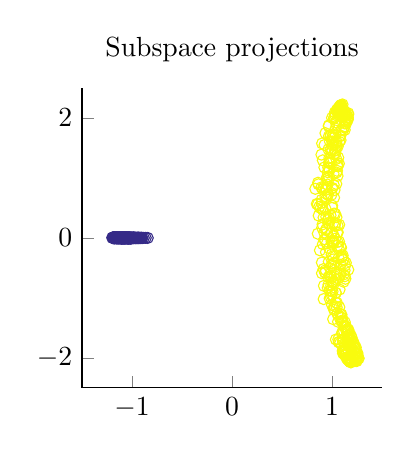
\begin{tikzpicture}

\begin{axis}[%
width=1.5in,
height=1.5in,
scale only axis,
colormap={mymap}{[1pt] rgb(0pt)=(0.2081,0.1663,0.5292); rgb(1pt)=(0.211624,0.189781,0.577676); rgb(2pt)=(0.212252,0.213771,0.626971); rgb(3pt)=(0.2081,0.2386,0.677086); rgb(4pt)=(0.195905,0.264457,0.7279); rgb(5pt)=(0.170729,0.291938,0.779248); rgb(6pt)=(0.125271,0.324243,0.830271); rgb(7pt)=(0.0591333,0.359833,0.868333); rgb(8pt)=(0.0116952,0.38751,0.881957); rgb(9pt)=(0.00595714,0.408614,0.882843); rgb(10pt)=(0.0165143,0.4266,0.878633); rgb(11pt)=(0.0328524,0.443043,0.871957); rgb(12pt)=(0.0498143,0.458571,0.864057); rgb(13pt)=(0.0629333,0.47369,0.855438); rgb(14pt)=(0.0722667,0.488667,0.8467); rgb(15pt)=(0.0779429,0.503986,0.838371); rgb(16pt)=(0.0793476,0.520024,0.831181); rgb(17pt)=(0.0749429,0.537543,0.826271); rgb(18pt)=(0.0640571,0.556986,0.823957); rgb(19pt)=(0.0487714,0.577224,0.822829); rgb(20pt)=(0.0343429,0.596581,0.819852); rgb(21pt)=(0.0265,0.6137,0.8135); rgb(22pt)=(0.0238905,0.628662,0.803762); rgb(23pt)=(0.0230905,0.641786,0.791267); rgb(24pt)=(0.0227714,0.653486,0.776757); rgb(25pt)=(0.0266619,0.664195,0.760719); rgb(26pt)=(0.0383714,0.674271,0.743552); rgb(27pt)=(0.0589714,0.683757,0.725386); rgb(28pt)=(0.0843,0.692833,0.706167); rgb(29pt)=(0.113295,0.7015,0.685857); rgb(30pt)=(0.145271,0.709757,0.664629); rgb(31pt)=(0.180133,0.717657,0.642433); rgb(32pt)=(0.217829,0.725043,0.619262); rgb(33pt)=(0.258643,0.731714,0.595429); rgb(34pt)=(0.302171,0.737605,0.571186); rgb(35pt)=(0.348167,0.742433,0.547267); rgb(36pt)=(0.395257,0.7459,0.524443); rgb(37pt)=(0.44201,0.748081,0.503314); rgb(38pt)=(0.487124,0.749062,0.483976); rgb(39pt)=(0.530029,0.749114,0.466114); rgb(40pt)=(0.570857,0.748519,0.44939); rgb(41pt)=(0.609852,0.747314,0.433686); rgb(42pt)=(0.6473,0.7456,0.4188); rgb(43pt)=(0.683419,0.743476,0.404433); rgb(44pt)=(0.71841,0.741133,0.390476); rgb(45pt)=(0.752486,0.7384,0.376814); rgb(46pt)=(0.785843,0.735567,0.363271); rgb(47pt)=(0.818505,0.732733,0.34979); rgb(48pt)=(0.850657,0.7299,0.336029); rgb(49pt)=(0.882433,0.727433,0.3217); rgb(50pt)=(0.913933,0.725786,0.306276); rgb(51pt)=(0.944957,0.726114,0.288643); rgb(52pt)=(0.973895,0.731395,0.266648); rgb(53pt)=(0.993771,0.745457,0.240348); rgb(54pt)=(0.999043,0.765314,0.216414); rgb(55pt)=(0.995533,0.786057,0.196652); rgb(56pt)=(0.988,0.8066,0.179367); rgb(57pt)=(0.978857,0.827143,0.163314); rgb(58pt)=(0.9697,0.848138,0.147452); rgb(59pt)=(0.962586,0.870514,0.1309); rgb(60pt)=(0.958871,0.8949,0.113243); rgb(61pt)=(0.959824,0.921833,0.0948381); rgb(62pt)=(0.9661,0.951443,0.0755333); rgb(63pt)=(0.9763,0.9831,0.0538)},
xmin=-1.5,
xmax=1.5,
ymin=-2.5,
ymax=2.5,
title={Subspace projections},
axis x line*=bottom,
axis y line*=left
]
\addplot[scatter,only marks,scatter src=explicit,scatter/use mapped color={mark=o,mark options={},draw=mapped color}] plot table[row sep=crcr,meta index=2]{%
-0.953966026969266	6.0036873244967e-05	-1\\
-1.0665588327701	0.00164135341208124	-1\\
0.963588321920559	-0.652498581685229	1\\
1.15867385206837	-2.01486407344045	1\\
1.25399474353282	-1.91971019040594	1\\
1.06973888186878	-0.0611840220556161	1\\
0.976239969655869	-1.010056945069	1\\
-1.15055255715601	0.00294418451675058	-1\\
-0.943022530875931	0.00196552405199222	-1\\
-1.07796351647924	-0.00343534773770568	-1\\
-1.10808307069589	0.00347933138570754	-1\\
0.905556267982138	0.224248028480711	1\\
1.04466754155752	-0.573292335162527	1\\
0.917592652668306	0.838721289843633	1\\
1.22983361318767	-1.82943017704745	1\\
1.04221238351492	1.61619181506799	1\\
1.00124502882711	0.537768841228339	1\\
0.969486055481423	1.69770854038497	1\\
1.0574582690458	0.092097010054196	1\\
-1.12056041981896	0.00416336164577065	-1\\
1.1278626394837	1.94584629451897	1\\
-1.18459710548508	0.00458715524205839	-1\\
-1.12802147518448	0.00419366756057603	-1\\
-1.13814940146636	-0.0049987106526915	-1\\
-1.05647303689791	-0.00432498650764852	-1\\
-1.03614081550618	0.0023137513974609	-1\\
1.03673999747196	1.92497754899503	1\\
-0.946910569841818	-0.0019499848314891	-1\\
1.08653512259394	2.14328112349182	1\\
1.0253875635756	0.79771244247968	1\\
-1.13938050014556	0.00273128004040653	-1\\
0.979445168312215	-0.635953498509566	1\\
0.991484100395172	-0.65426467597282	1\\
-1.12478297193685	-0.0034419552665026	-1\\
1.0203893766933	0.670167759420234	1\\
-1.07745872131767	-0.000819920655951679	-1\\
1.00156469861947	1.60693015604847	1\\
-0.986996281466881	-0.00237814063988215	-1\\
1.23449981414552	-1.99424217687806	1\\
1.18904012148804	-2.04540187635714	1\\
1.07174891441888	0.218244903627844	1\\
0.959049614078562	0.717186786356942	1\\
1.0175758422613	-1.16772096766899	1\\
-1.10578951069085	-0.00538539674196209	-1\\
0.961705669160374	1.17607264235659	1\\
0.866134879558377	0.370086501183963	1\\
-1.07661888628023	0.00360799445317511	-1\\
-1.06277167505748	-0.00516088259530108	-1\\
-1.08122974552147	0.00323674312040162	-1\\
-1.17566717384095	0.00446895868945683	-1\\
1.12387674261101	-1.8795982121079	1\\
0.959339157508341	0.731274998308441	1\\
-1.17947199145204	-0.00495028192107815	-1\\
1.05414437016214	-0.0667865109888285	1\\
-1.08784985282971	-0.00489764224263628	-1\\
-1.00629691598834	-0.00104267511675617	-1\\
-1.06247951687831	0.00124017838583957	-1\\
-1.11263288080717	-0.0054486281462222	-1\\
-1.05206036780052	-0.00124221433781325	-1\\
-0.93845997441135	-0.00182459176799762	-1\\
0.929135774097109	-0.0274856212818571	1\\
1.0703127702001	-1.3074671295858	1\\
-1.19044364064795	0.00455716275886201	-1\\
-1.15058235195723	0.00340928701465412	-1\\
1.05487910999412	0.207731007556065	1\\
1.12848470675301	1.90590845546068	1\\
-0.979666790047988	-0.00209066808572619	-1\\
0.988853874478545	1.47191984427225	1\\
0.964216464200042	1.47784698791807	1\\
1.0901801367868	2.21183469242423	1\\
-1.11988424042591	-0.00375212657551255	-1\\
-1.06934210456882	0.00392010775653622	-1\\
1.25045701498556	-1.99986299155078	1\\
-0.986456042840513	0.000394529492526691	-1\\
-1.07516322104345	0.000312003349173121	-1\\
-1.08606788021442	0.00311569631142909	-1\\
-1.15629714306377	-0.00506944942941848	-1\\
1.00888346054974	-0.730778000421887	1\\
0.939170069581612	-0.237968884426363	1\\
0.90135765968391	0.169683511094886	1\\
-0.981787358618003	0.00111138262880571	-1\\
-1.065953344173	-0.000236657568750832	-1\\
-0.972539833926744	-0.00029096049042961	-1\\
-1.04817826697326	0.00144913832999361	-1\\
-1.0366991420919	-0.00253669091073996	-1\\
1.05478683871414	1.03220672572807	1\\
0.972444539577578	1.11652511735398	1\\
1.25513947974171	-1.95796267448503	1\\
-0.959645328557816	-0.00170714906511299	-1\\
1.06846051069284	1.23817047719273	1\\
0.959912260765105	0.956222524916275	1\\
-1.13562122091033	0.00424426863534724	-1\\
-1.08930926685103	0.00370981200685867	-1\\
0.952423359472407	1.0203758628267	1\\
0.970062483825138	1.15465049192981	1\\
-1.04204028560447	0.000877724100473929	-1\\
1.05071520104005	2.11328026478226	1\\
1.05520734945216	1.21786518755854	1\\
1.10618041989359	-1.38750345161049	1\\
-1.15966100488049	-0.00504126239891034	-1\\
1.09342483734236	-0.329938554725957	1\\
-1.0302585305176	-0.0032048990180541	-1\\
-1.05856940200359	0.000551600338820197	-1\\
-1.09944843394035	-0.00546969591511683	-1\\
-1.07692101843024	0.00366905097411271	-1\\
-1.05674033221476	0.00140528589434212	-1\\
1.1627635236292	-0.530746290644895	1\\
1.07693442394841	2.1601391824535	1\\
-1.09489722290143	-0.000136410381510391	-1\\
1.14337583566553	-1.55016744664882	1\\
-0.972380545036134	-0.00182165031466049	-1\\
1.03825581281302	-0.917303382026377	1\\
0.93445275656433	0.485524967783866	1\\
1.17838307148714	-2.05866333780803	1\\
-1.04007656084063	-0.00464154067578465	-1\\
0.89426104448784	0.841854948658276	1\\
1.15815344221005	2.00118682997302	1\\
-0.984306566441328	-0.00219459206693638	-1\\
1.09581122544699	2.19359936558532	1\\
0.938591443962709	0.130202873883011	1\\
-0.95354566968336	-0.001816313315095	-1\\
-1.04400598254119	0.00149978568755815	-1\\
1.12533710509662	-1.47704116747061	1\\
-1.10114881995376	-0.000324822109273834	-1\\
-1.00117377093245	-0.00255001538312039	-1\\
-1.16164850081491	0.00438909621282037	-1\\
1.07712286889007	2.1655353026947	1\\
-0.986977260599904	0.00133442676962834	-1\\
1.24287085238126	-2.03456303986612	1\\
1.08999001872233	-1.3841910789621	1\\
-1.15774088580732	-0.00490871963983467	-1\\
1.1290127977335	2.0877311950559	1\\
0.9345448936491	0.692755085966346	1\\
1.05085754838588	2.1228336074158	1\\
1.26644063975124	-2.01000193492816	1\\
-1.1686089199976	-0.00444350913361025	-1\\
1.02415886968346	2.01559647028228	1\\
-1.07928485450961	-0.00285344606653811	-1\\
-1.1661259062257	0.00303142817814645	-1\\
-1.07115055220182	0.00319891915555914	-1\\
1.09227721857731	2.21256254294314	1\\
-0.84316484730677	-0.0010382685641994	-1\\
-1.00449993217592	-0.00421642339589676	-1\\
-1.0634472379979	0.00223027874048295	-1\\
-0.922298407535141	-0.00243643608803775	-1\\
-1.03690948067006	-0.00310796289770296	-1\\
0.908230805927848	-0.104831163897187	1\\
1.17083850255182	-2.04547740781666	1\\
1.12467076417086	2.11235831582212	1\\
1.05294322280009	-1.26485387511285	1\\
1.17427072602151	-1.60740119972605	1\\
-1.10115800993366	-0.0049295584913625	-1\\
-1.06574581114327	-0.00509190076492242	-1\\
-1.12986572010909	-0.0040808348303407	-1\\
-1.08127874050126	-0.00518699720010852	-1\\
-0.953883279809735	-0.00148827020315184	-1\\
1.06928255848434	2.07657651200375	1\\
-1.002069623395	0.000108486336915241	-1\\
-0.919721749962428	-0.00248433571878088	-1\\
-1.04086616823135	-0.00392150427239067	-1\\
0.864055986644835	0.892811132704106	1\\
-0.968970902717145	-0.0017569981374363	-1\\
1.04284768666207	1.31463220476923	1\\
-1.18091638428259	0.0044935808394947	-1\\
0.906347477148193	0.809391815328305	1\\
1.10013389154406	2.08168822224803	1\\
-1.02807969551213	0.000388450963682908	-1\\
-1.03056802522481	0.00119257809557502	-1\\
1.14025745657706	-1.47916329289543	1\\
-1.07629524740108	0.00220315916434391	-1\\
1.1244793616087	-1.81930288985003	1\\
-1.08641219470678	0.00351388213509401	-1\\
1.15459106170529	-1.52203724862971	1\\
-1.08120526796697	-0.00361901793421078	-1\\
-1.0523288815064	-0.00347700397945745	-1\\
-1.07120074612473	-0.000912736228582744	-1\\
1.02621745005012	0.200886306158433	1\\
-1.18224930519675	0.00299461493206989	-1\\
1.17034125150554	-2.04478264706571	1\\
-1.04341188293142	-0.00499402241234475	-1\\
1.00989303633428	-0.738070974502745	1\\
1.07229071307978	2.05550528479973	1\\
-1.10701164674562	-0.00545831860737476	-1\\
-1.04245705134283	0.00114385920955145	-1\\
1.03359607327236	1.722641861734	1\\
-1.09177861240992	0.00403140797909471	-1\\
-1.05679082635526	-0.000970063992210764	-1\\
-1.1407777444016	-0.004633381111619	-1\\
1.03733943014277	1.58646328146949	1\\
1.11476926546552	-0.367212647183672	1\\
0.860186083353512	0.919431580437719	1\\
1.07060599913619	-1.73568790888567	1\\
1.16681397977212	-1.77924624657881	1\\
-0.940796202754507	-0.000946550762912677	-1\\
1.03610966927614	-1.07694153074709	1\\
-1.08045466168875	-0.00538621336059307	-1\\
-1.08139781787556	0.00335424272413356	-1\\
-1.13945129936637	-0.0043984683540445	-1\\
-0.967147926873053	0.00252892629150928	-1\\
1.15814574136104	-2.00112175348212	1\\
1.07119439655616	2.14775928773561	1\\
-1.17714911482888	0.00462049688223221	-1\\
1.09058124402484	-0.162963984620157	1\\
-1.01355108670045	0.00211117028198789	-1\\
1.08500887962728	-0.44883819687529	1\\
1.04453007589667	0.344593228451249	1\\
0.857353569789071	0.0695090554064951	1\\
0.957730334585171	0.297203255604153	1\\
1.14936242371228	-1.75436434534622	1\\
1.15380717094361	-1.59200460697878	1\\
1.26171057690332	-2.00147582082775	1\\
-1.01538622009364	-0.000318864850721233	-1\\
-1.09050804458464	0.00342475643689406	-1\\
0.847853505212812	0.565568473357938	1\\
-1.06668291318898	-0.000859494982711565	-1\\
1.11615246458507	-0.610355530321261	1\\
1.19175094268997	-2.04872800043406	1\\
-1.04497336928918	0.00154672235848455	-1\\
-1.10527527119611	-0.00468263826364846	-1\\
-1.0426937978232	-0.0050157855901297	-1\\
-1.1828548211608	0.00460777514325889	-1\\
-0.918851842828663	-0.00163723073101845	-1\\
-1.02275702364975	-0.00506749923459766	-1\\
-1.12777396747984	-0.00038530895095777	-1\\
-1.08726334816924	-0.0034924248398165	-1\\
1.12196533001665	-1.89522578852455	1\\
-1.03272918160817	0.00122680409621381	-1\\
-1.01838795326495	-0.00091477152808245	-1\\
1.10903718187139	-0.35812986512519	1\\
0.899227498328745	-0.589578382612502	1\\
-1.04943132507955	0.00161690494850006	-1\\
1.00168197644831	0.827583842768531	1\\
-1.0243264157551	0.00156273429960253	-1\\
-0.939439376647797	-0.000425155803108421	-1\\
-1.0955240033952	-0.00370066833996132	-1\\
-1.03352928833407	0.000667115661433928	-1\\
-1.15176082911902	0.00296870345620582	-1\\
0.923194033057287	-0.0245774258217894	1\\
1.06147287483467	-0.674866404811826	1\\
-1.07379647655002	0.00398197664164906	-1\\
-1.18946010625537	0.00458398506898108	-1\\
1.01211341578418	0.25338350298966	1\\
0.96779911059344	-0.396045932521682	1\\
-0.972712512479041	0.000521526116942131	-1\\
1.12965366431651	2.05778813913653	1\\
1.02006092036777	-0.752075193700419	1\\
1.07907856514327	-0.630199468516227	1\\
1.1274101609042	-0.639853792389025	1\\
-1.08396978481174	0.00386164177708142	-1\\
-0.927245445186036	0.000118160276455475	-1\\
-1.04558820092051	0.00255802353136325	-1\\
-1.01546289109145	-0.00455830817414514	-1\\
0.896509100447814	0.583132748621884	1\\
0.96632165372392	1.86259920240662	1\\
-1.17835352037198	0.00337392530144078	-1\\
-1.14829765107375	-0.00506127138664002	-1\\
-0.916303966838239	-0.000769014237493584	-1\\
1.16977976027128	-1.63382875665556	1\\
-1.05797585053975	-0.00527389493504941	-1\\
1.15875157366396	-2.0051591344737	1\\
-1.09336966518826	0.00412653711530989	-1\\
1.0033498365	0.832477396160394	1\\
1.18028557743519	-2.06129078366163	1\\
0.887076386305282	0.496436291667613	1\\
-1.02298867820013	-0.000502127808852857	-1\\
-1.14881398147618	0.00440914920797707	-1\\
-1.0691617081388	-0.00410036858150957	-1\\
0.925246395544379	1.54832274380263	1\\
1.04206181206846	1.50789355351989	1\\
-1.05568128719914	0.00378731780695919	-1\\
-1.07263088630845	-0.00374250920602189	-1\\
-1.11134952292291	0.00421524133366096	-1\\
1.10463595805507	2.22422422311637	1\\
-1.17252576252218	-0.00500541873039033	-1\\
1.01453728847937	1.07002273291971	1\\
-1.03609673889517	-0.00516280107903032	-1\\
-1.11994408271349	-0.000578062000535485	-1\\
1.0759889177804	2.16411183781688	1\\
-1.06041140000648	0.000709847320126093	-1\\
-1.07674612264861	-0.00536543593419004	-1\\
1.13373691097062	-0.681773472286879	1\\
-1.1405432900206	0.00442079967527095	-1\\
-1.01476093579435	-0.00456549819993256	-1\\
1.2325629585856	-2.05090688361527	1\\
1.0904945237015	2.2107525999808	1\\
-1.01743234478995	0.00037074376052488	-1\\
-1.05752195089378	0.0024771530607104	-1\\
1.16016257437251	-1.63192708539674	1\\
-1.12534605027539	0.00441091222500012	-1\\
-1.09411584367495	0.00409785118713605	-1\\
1.09214744101379	-1.33643312664317	1\\
1.0498887845974	1.11850969458569	1\\
-0.937769599504536	-0.00147385765743143	-1\\
1.10002409394667	-1.39504172368858	1\\
-1.1081687607355	-0.00548257539262771	-1\\
1.06264781499902	-1.69160373479294	1\\
1.087778299575	2.20505058632645	1\\
0.963235486748429	0.243817420325195	1\\
-1.10028142234854	0.00291529788665034	-1\\
-1.12045845851342	0.0027913710670993	-1\\
-1.0289502249515	6.43249700562568e-05	-1\\
-1.06882760352486	0.00370800180511866	-1\\
-0.908474125672774	-0.000478841405945579	-1\\
-1.03712024397203	0.000248422808016659	-1\\
-1.04030474253522	-0.00518097977338648	-1\\
-1.03111740060105	0.000664895898964649	-1\\
1.07184478050626	1.60077570501068	1\\
-1.01588417226154	-0.00502528091354365	-1\\
-1.10947020526556	-0.00543064129319504	-1\\
0.936993263343374	-0.538924073913888	1\\
-1.13987368186097	0.00435598389806704	-1\\
1.09426028105498	-1.27882392328059	1\\
-1.05790292274673	0.00371961099638597	-1\\
1.13935631195922	-1.93351696000651	1\\
1.24373811507231	-1.97609710871208	1\\
-1.14598976061492	-0.00495928237817546	-1\\
1.18588093838733	-1.61964803088983	1\\
-1.00498385657651	0.00177656166272248	-1\\
0.923396477510349	1.17474797665967	1\\
-1.00091072698045	-0.00313166160871351	-1\\
1.01907989185243	1.99377184603292	1\\
-1.17651012078149	0.00337080915448645	-1\\
-1.09749748562201	-0.00421348380203742	-1\\
1.0662180670707	2.16628279656025	1\\
-1.16996774456912	0.00457013827453669	-1\\
-1.1532268527722	0.0043869002676514	-1\\
1.03855055708632	-1.69442824752952	1\\
-1.10083164312898	-0.00545482839411398	-1\\
-0.882438273549477	-0.000259789289404999	-1\\
-1.02554266214167	0.000241491267533516	-1\\
-1.06086313967013	0.0003830494521106	-1\\
1.00331038898982	1.55451781299681	1\\
-1.12617606916567	-0.00459003896601997	-1\\
1.07178782424707	2.08030014882614	1\\
-1.18088509925228	0.00458252716299562	-1\\
-1.02292259988842	0.00144533759634953	-1\\
0.989536866493325	1.25873412497999	1\\
1.11483660595511	2.07877720023966	1\\
-1.05499220036549	0.00182469464181561	-1\\
-1.08434137589466	0.00393390895089362	-1\\
1.08214779473607	2.19900193355377	1\\
0.934043793283153	1.74538884907687	1\\
1.10933658125461	-1.87264837186641	1\\
1.08326613441494	2.13860804383935	1\\
-1.05754013347484	0.000558273699300874	-1\\
-0.991170007665649	0.00126866885402742	-1\\
-1.11231491419947	0.00239936787553568	-1\\
0.986838694639467	1.71893162578827	1\\
1.19582222706617	-1.66108048510872	1\\
1.18832816541755	-1.71130869234828	1\\
-0.898037871143567	-0.0020150475094611	-1\\
-1.18754700001603	0.00463873363228881	-1\\
1.03562201171932	1.82231728285758	1\\
-1.18974855305674	0.00464149768992813	-1\\
-1.09435338032368	-0.00335797010792434	-1\\
1.02781637747765	-0.413415064988888	1\\
-1.07974066207211	-0.00394247758691615	-1\\
-1.01772165084725	0.002711091681356	-1\\
-1.07573683853458	0.00385888288535421	-1\\
-1.03734570937334	0.00209198334857653	-1\\
-1.04943879879804	-0.00522228956211881	-1\\
0.970065913025979	-0.170760161715152	1\\
1.03195155698265	0.399450149422955	1\\
1.15473464053822	-1.99707400132019	1\\
1.19502289220787	-1.84787364242546	1\\
-1.05472872959225	0.00190858475069015	-1\\
1.07705623092702	2.11421913282297	1\\
-1.10103033583449	-0.00497144382855052	-1\\
-1.0296632666747	0.00150206160121607	-1\\
-1.1181911848491	-0.0035779008816178	-1\\
1.06542938151992	-0.334993431040051	1\\
1.01099933622962	-1.35474548150987	1\\
-1.09121836071789	0.00409481216964146	-1\\
1.18589540301265	-2.06885319420166	1\\
1.08453354647669	2.18755750567748	1\\
-1.17898005523228	-0.00462543128224452	-1\\
-1.19812754964137	0.0032510349583636	-1\\
1.13126873469489	-0.45906918355793	1\\
-1.12288214858118	0.00430191982430058	-1\\
-1.06681286696265	-0.00531782999929325	-1\\
-1.17715111348491	-0.00494163714192915	-1\\
1.05427870539144	-0.126915777290495	1\\
0.969057094264932	1.87666763499037	1\\
-1.17257269482367	0.0045140170283708	-1\\
-1.07455350774215	-0.00535736204221165	-1\\
1.01460429745401	-0.429000395645917	1\\
-1.09488109779312	-0.00543675048919278	-1\\
-1.04455205122485	0.00276905983148128	-1\\
0.915532862593647	-0.519417010653955	1\\
1.23282635307955	-1.92239753204387	1\\
-1.01226489694991	-0.0048059571256921	-1\\
1.13536978854133	2.0509879885665	1\\
-1.12305862617578	-0.00382966034154621	-1\\
1.18010509717125	-2.03005716690674	1\\
1.15178081586754	-1.73557627625473	1\\
0.992399592379167	-0.876944583745824	1\\
-0.987902746005608	0.000572012655082711	-1\\
1.01860635779312	-0.0629096635069558	1\\
1.24009036867853	-2.00118513951818	1\\
-0.941357508469246	-0.00241880744001739	-1\\
0.878553602517766	-0.207583585179591	1\\
1.06683364276702	-0.182481854468508	1\\
1.18661829841521	-1.76488466952396	1\\
1.12031617202617	1.85430060111542	1\\
1.1884120271262	-1.7191443339771	1\\
1.0124215752976	-0.358865184908684	1\\
1.03796814316897	-0.693238063899661	1\\
1.09301374398119	2.12018718377756	1\\
1.0121555283219	1.59325069295749	1\\
-1.05155078679171	0.000839369939335141	-1\\
-1.090748778764	-0.00398469853908821	-1\\
1.01607474624956	1.39336418926803	1\\
-1.06177889142979	0.00304630793680455	-1\\
1.08510270284601	1.62815898690211	1\\
-0.933051406944463	-0.00133674996977291	-1\\
1.09818490826503	-0.309788016415805	1\\
1.16191869058386	2.05780676650603	1\\
-1.07057663187065	-0.00515834774193818	-1\\
0.895995363540356	0.633157581666949	1\\
1.08800353650766	2.12620538780472	1\\
1.10768906448864	-1.88563657104733	1\\
0.969767927632223	0.332092810752694	1\\
1.13019291927803	2.05722093421067	1\\
0.979280345401618	1.605127767207	1\\
-1.06976891261176	0.00372544560662928	-1\\
1.15398963077559	-1.5421915948326	1\\
-1.03654717230326	-0.00465061523510876	-1\\
1.12179015860396	1.84000858488738	1\\
-1.09851291122474	0.00244049498176265	-1\\
-1.19103223161631	-0.00496592169941014	-1\\
-1.15824806625946	-0.00487954295643549	-1\\
1.08182077698004	-1.26590638527484	1\\
-1.12909264271373	-0.00415493120113651	-1\\
1.07281420481323	-1.15399930462318	1\\
1.15602883996338	2.01409349075201	1\\
-1.18505153466818	0.00460980493032582	-1\\
-1.14576901877485	0.00277999282751222	-1\\
0.918695304200669	-0.799288919448299	1\\
-1.00890061190223	-0.00273256077299158	-1\\
0.99304784229463	-0.460958245849403	1\\
1.08391441360479	2.1908036974731	1\\
-1.02774322666493	0.00211951218422175	-1\\
-1.15356998165865	0.00438362529427366	-1\\
0.984681474857554	0.375182336570234	1\\
-1.01218394995977	-0.00482681247363831	-1\\
0.995850399953451	-0.948707251351353	1\\
-1.17478415601256	0.0044707931289226	-1\\
-1.0082455663432	-0.00423153123254379	-1\\
0.995525173247241	-0.062367405570917	1\\
1.1205913248247	-1.5612726403183	1\\
1.1636771850772	-2.03298007431933	1\\
1.00230267552701	1.46476208136379	1\\
1.00021577961177	-0.742855654064394	1\\
1.20740984327893	-2.0342747082008	1\\
-1.18162917235033	-0.00482569698442243	-1\\
1.1155359818021	-0.731495475553726	1\\
-1.07304887912129	0.00407443657703187	-1\\
1.09529029539347	2.0845670145637	1\\
1.16322252106365	-1.67195793592686	1\\
1.21655792703162	-1.75278143508509	1\\
-1.0732897125382	0.00371090709691415	-1\\
1.18315637069341	-2.01119370556127	1\\
-0.964665756363398	-0.00269621105519878	-1\\
-1.02325662323516	-0.00502117391237797	-1\\
0.931286453444983	-0.572847578935774	1\\
1.05987940694339	2.14025383556288	1\\
-1.00642243960204	-0.00293563770039454	-1\\
-0.963031981323578	-0.00196113191429873	-1\\
-1.10900936563847	-0.00481190231850068	-1\\
0.973578557211543	1.33332529959485	1\\
0.945948036621805	0.669829019740908	1\\
1.04966707330329	1.20897264828229	1\\
-1.13368616921185	0.00350756179335499	-1\\
-0.99688606686741	0.00112074441476051	-1\\
-1.0537804814694	0.00347197030651289	-1\\
1.19120160869338	-2.05029478048069	1\\
1.2464710114532	-2.05394364184191	1\\
-1.06140299843809	0.00379207943766974	-1\\
1.0299976082036	-0.0147555391607795	1\\
1.1270281061573	1.7987583917834	1\\
1.13241480941655	-1.93826851613642	1\\
1.18427889482928	-1.69909682728431	1\\
1.15444167970913	-2.01270965740251	1\\
1.10632796917432	2.03279924580859	1\\
-1.07297744021715	0.00282432837721546	-1\\
-1.15903437269128	-0.00383201315778807	-1\\
1.14197334653158	1.93680221828659	1\\
-1.0870819851677	0.00260413501779781	-1\\
0.832897143657809	0.817086725974304	1\\
-1.12824344421939	-0.00392148839172096	-1\\
-1.03754081222488	0.00123628090716905	-1\\
-1.10151020297555	-0.00320181159376736	-1\\
-1.06521810907399	-0.0051119655938026	-1\\
0.987484637889399	-0.986356667992844	1\\
-1.02848304538267	0.0020514671234652	-1\\
1.03602418763255	1.457320734949	1\\
1.16442575506731	-1.53408310473337	1\\
-1.09350634978921	-0.00541464231959549	-1\\
-1.08599722766172	0.00375965461022054	-1\\
-0.996263507117493	0.00316882487585797	-1\\
1.06216588629077	1.33688989737681	1\\
1.14679948037314	2.05432031797581	1\\
0.915242884415478	0.337404296923277	1\\
1.07354257144914	2.18102729358971	1\\
1.12548218157958	-0.542544849957232	1\\
0.921918413201384	0.090508571915084	1\\
-1.06652956658422	0.00361844495653701	-1\\
1.08492972534996	1.70675833127954	1\\
-1.01638758818142	-0.00493801116085529	-1\\
1.08421677147874	2.20064155370379	1\\
0.939739502285035	0.835891437350689	1\\
1.16471799459515	-1.69099408708867	1\\
1.13823971250827	-0.415804434532857	1\\
1.1601926781472	-2.0260238331623	1\\
1.21425729169861	-1.77576690200577	1\\
-1.06413170140592	0.000952982625048116	-1\\
-1.01857651967121	0.00156212927003527	-1\\
-1.03100908468134	-0.00496454801045543	-1\\
1.05323795618245	2.09745542536798	1\\
-1.09204392872546	0.00401665558527688	-1\\
-1.10138213667057	-0.00499452542526923	-1\\
1.04622748503426	-1.15512137019952	1\\
1.08176511865311	-1.75240880866153	1\\
-1.05803008382149	-0.00121942490509065	-1\\
1.10283822346647	-1.57130094020355	1\\
0.995622034022317	-0.276690944810137	1\\
1.22998288316995	-2.03262922171175	1\\
1.20075890081552	-2.05806449285157	1\\
1.17820401215808	-2.05937482546615	1\\
-1.13948797267299	-0.00396423841242285	-1\\
0.973995990508367	1.24314144744802	1\\
-1.07635041938964	-0.00485465344704918	-1\\
-1.09221778613151	9.8330791955831e-05	-1\\
-1.06535916340722	0.00390428566911235	-1\\
-1.03480417211576	-0.00494073851339651	-1\\
1.1889342027021	-2.07580668951011	1\\
-1.072018703376	-0.00101238308053437	-1\\
1.16193480909845	-1.74498871558189	1\\
1.1418805825974	2.03071648066625	1\\
-1.0385574571648	0.000216153042814839	-1\\
1.18207692737999	-2.06524748895094	1\\
-1.06732492151452	-0.00364679190034597	-1\\
1.00412306356267	1.68089780636062	1\\
-1.06247672954143	0.00327222933877843	-1\\
1.23010136008668	-2.02122016632604	1\\
-1.08572266790144	-0.00476689089109918	-1\\
1.08499693740283	-0.148839247916963	1\\
-1.0824677753839	-0.00405191828591473	-1\\
-1.10483559773887	0.00415119237201537	-1\\
1.18171061276845	-2.00487172070906	1\\
-1.03187045952524	0.00345231091531153	-1\\
-0.97935010366015	0.00227910283019389	-1\\
0.90057237709676	1.57385281664605	1\\
-1.11123818054196	0.00423525910657602	-1\\
-1.01739147744051	-0.00416649792395725	-1\\
1.03016718895004	2.05316304238196	1\\
1.05186773682665	2.10902844180727	1\\
1.10645802281398	-0.290897628858287	1\\
0.931470844739547	-0.583736854128319	1\\
1.12265357306917	-1.93996011614343	1\\
-1.05406151527455	-0.000707253281178209	-1\\
-1.09412704256072	0.00375902287187916	-1\\
-1.0903628230731	-0.0052884217025907	-1\\
1.06610056690689	-1.73757928586751	1\\
1.24318359850668	-2.04088747079833	1\\
1.07029503028989	2.12970417625704	1\\
1.10940190564776	-1.9228659159002	1\\
-1.03945314489003	-0.0029591714147744	-1\\
0.968048273612279	1.02642271552153	1\\
1.16743247198601	-1.80675500440666	1\\
-1.04349833526134	0.00132065953081891	-1\\
-1.10496733039559	-0.00547636253134761	-1\\
1.14540194638241	-1.939015369441	1\\
-1.02607762209452	-0.00350834447474847	-1\\
-1.06533083644297	0.00265784734882606	-1\\
-1.09685330058562	0.00340233645106765	-1\\
1.06024137360133	-1.39797030019466	1\\
1.14388288463954	-1.99640972965157	1\\
-1.13805276446673	-0.00426625011523137	-1\\
-1.14005419265679	0.00345682223417008	-1\\
1.03292763922587	0.243824259325243	1\\
-1.1162363607183	-0.00324494514016275	-1\\
1.00971055759548	-0.305504227165438	1\\
-1.04604578281685	-0.00492961051353266	-1\\
1.07281922050563	2.12597673615809	1\\
0.943177310725639	0.146310883869041	1\\
-1.08195623014354	-0.00499808845922768	-1\\
-1.00322100848918	0.00102139866323239	-1\\
0.976833446367247	1.28438476108824	1\\
-1.08800320774985	-0.000198695707196686	-1\\
1.0070382073922	-0.0458034123613347	1\\
-1.03819209471908	-0.00390382346958988	-1\\
-1.16112618773229	0.00442841337189985	-1\\
-1.04944564540781	-0.00488979838022629	-1\\
-1.14078540939456	-0.00470518415512436	-1\\
1.21986753620103	-1.96500790739256	1\\
1.01503115233543	-0.0780279327584778	1\\
-1.18563979093897	0.00316403303282725	-1\\
-1.07426084176458	0.00341787062335104	-1\\
-1.02113581588798	-0.00486292831275383	-1\\
-1.11819845937873	0.00327015171791891	-1\\
-1.10733872592815	-0.0042005638499848	-1\\
1.18921634058308	-2.0051066566709	1\\
0.956679349695215	1.0936654186601	1\\
-1.1124414819832	0.00319253074955522	-1\\
-1.05666691206224	-0.00484183109868814	-1\\
-1.01600676337343	-0.000414143861183256	-1\\
0.942359240967912	0.351442722983169	1\\
-1.08379588225791	0.00350267982222748	-1\\
1.04256017536394	0.899215240503158	1\\
1.01514699236001	0.0394923632100963	1\\
-1.03414016756367	-0.00459028508137131	-1\\
1.16153750628149	2.07685070535628	1\\
-1.11706928588888	-0.00332338513035059	-1\\
1.05410265352146	2.143217528494	1\\
-1.01554946966833	-0.00417842626539833	-1\\
1.05147724960875	-0.618523430816434	1\\
-1.0601273855215	-0.00405098787551351	-1\\
1.03177588153184	1.46032037495689	1\\
1.01112513697913	1.66154904959703	1\\
-1.10635177541874	-0.00548181429231536	-1\\
1.17417862415904	-1.74878667582422	1\\
1.23765030587288	-1.82421192500007	1\\
1.00004694754057	0.0914253991961594	1\\
-1.15556730918676	0.00450604347176915	-1\\
1.04298492181441	1.92142178601238	1\\
0.985419628586236	1.69288713550346	1\\
-1.12915295398305	-0.000287622789155656	-1\\
1.12760102569457	-1.40396194386802	1\\
-1.10288703406254	0.00424670295942121	-1\\
1.16008736343842	-1.5495746576726	1\\
1.23784364065998	-1.93304714218001	1\\
1.14186787357781	1.91147670593322	1\\
-1.02460400013642	-0.00470934612664936	-1\\
1.04901247344627	1.96116626468394	1\\
1.06460823329328	2.10918040064448	1\\
-0.976208257595927	-0.000399379709500756	-1\\
-1.09593137606702	-0.005414093562199	-1\\
-1.04494357344488	-0.00357368511042418	-1\\
0.999960460211412	2.00051162874876	1\\
-1.05463208921368	0.00221231692398755	-1\\
-1.11073394767447	0.0026041795768053	-1\\
1.24987428905532	-1.9809176673677	1\\
-1.03142976079675	0.00279922577920499	-1\\
-1.04997236601181	-0.00486399683037557	-1\\
1.15740590513824	-1.56021033857607	1\\
-1.08580442832487	-0.00286119784707086	-1\\
-1.00406846325676	0.000270881330741106	-1\\
-0.932323508838828	-0.000402277549996528	-1\\
-1.08880824034011	0.0038549661265606	-1\\
-1.07796596892322	0.00326367380983387	-1\\
-1.09594496506888	-0.0042795282685583	-1\\
-0.970447231329548	-0.00113155109417848	-1\\
1.01728079453653	0.883030057111752	1\\
-1.12710125521036	0.00419511254341121	-1\\
-1.01725656305122	0.00328708135428668	-1\\
1.16721419847433	-1.89918106571492	1\\
1.18796222608554	-2.02566290934602	1\\
-1.03278312951139	-0.00253157724992275	-1\\
-0.987239762548324	-0.000200599785672898	-1\\
-1.07683631340799	-0.00300264251465612	-1\\
0.971373603622043	1.25878971456502	1\\
1.07979866917985	2.12134964268602	1\\
1.05683518145413	1.52233264106739	1\\
-1.10440122141444	-0.00547846087829558	-1\\
-1.0731978952249	0.00239168510485614	-1\\
-0.942652541247784	-0.0010389110355997	-1\\
0.957442416668291	-0.831935755406666	1\\
1.09956340671656	-1.60133971870908	1\\
-1.07855399367315	-0.00356596795549247	-1\\
-0.936104798989355	8.07660718932836e-05	-1\\
1.08426353701031	2.19525280071529	1\\
1.15210259005446	1.96951432916265	1\\
-1.07397531387876	0.00222717503898902	-1\\
-1.03954863805754	0.00280293061024278	-1\\
1.01986670963672	-1.19724149876827	1\\
1.12490595831218	-1.47060756450748	1\\
-1.03101151673332	-0.00507032366239993	-1\\
-1.09312204878083	0.00397048410962228	-1\\
1.13084549865026	-1.95742193923539	1\\
0.993836740109743	0.718024637561841	1\\
0.978789309176653	-0.50263335106716	1\\
1.06278754956081	2.08514427970399	1\\
1.07794964062914	1.69057653665433	1\\
1.22008766737072	-1.82191970936849	1\\
-0.993181786907042	-0.00481537171534391	-1\\
-0.906341062745881	0.00146391583193279	-1\\
-1.02828177711742	0.00348032338911812	-1\\
1.00892473083143	1.71788798603436	1\\
1.18987895189106	-1.82412303755574	1\\
1.0476409566378	2.12880285871455	1\\
-0.988363356833631	-9.34240833940898e-06	-1\\
0.968563591971823	0.249897428083883	1\\
0.977486546105857	-0.879513140425065	1\\
-1.13383102739176	0.0031814904749373	-1\\
1.04483881697009	1.08977135643119	1\\
1.16055354810529	-2.02952665345216	1\\
-1.12601497373322	-0.003866896858758	-1\\
-1.11427188980827	-0.0054626982013379	-1\\
1.10881058142154	-1.71348300799431	1\\
-1.04250644285751	-0.0048518486827586	-1\\
-1.12559888413817	-0.00345991557712127	-1\\
-1.06796526021646	0.00302674255904601	-1\\
-1.07053633079147	0.00348752866671167	-1\\
1.22245330011052	-1.83897880146406	1\\
1.04673540594179	1.53605488638355	1\\
1.03326379566849	1.41376709281578	1\\
0.99991626849037	0.500741236233956	1\\
-1.06446988597885	0.00310440425274197	-1\\
-1.034266231836	-0.00264808977041989	-1\\
-1.1502605288784	0.00440748048801499	-1\\
-1.03998970060512	0.00198005972398242	-1\\
-1.16674549266454	0.0032378627336956	-1\\
-0.940390941266723	-0.00131966540259563	-1\\
1.25054772102795	-1.93643333306556	1\\
1.02879834916036	2.09223083352537	1\\
-0.985339072271978	0.000135750171793894	-1\\
-1.08453772763487	0.00379916695132369	-1\\
-1.03535585575658	-0.00456902995740855	-1\\
1.10869602462795	1.79413900892682	1\\
-1.11952339017888	0.00320306639108917	-1\\
-1.10853778079423	-0.00472529684165939	-1\\
-1.05021568565174	-0.00304233594010502	-1\\
1.20972286225136	-1.73169074559378	1\\
-1.10267274789918	-0.00394887516480031	-1\\
1.11655092191515	-1.68890079965371	1\\
-1.08169061496411	-0.00404981296313371	-1\\
1.04849771771368	-1.08313009969053	1\\
-1.06983013157677	-0.00495982314914791	-1\\
1.00032602841671	-1.11894381015628	1\\
1.1758139846681	-2.05343067193902	1\\
0.98940450642731	0.0790446085161393	1\\
-1.09974570241701	-0.000635728685823614	-1\\
1.05069379882217	0.0888690178803873	1\\
0.916171224732074	-1.02055162005713	1\\
-1.03922372943573	-0.00517652263003211	-1\\
-1.06590498833787	0.00363178754377348	-1\\
0.906963206053719	0.471200499981023	1\\
-1.01948467544271	-0.00503645571406532	-1\\
-1.02564822523593	-0.00491218738124269	-1\\
-1.14514436820303	-0.00342744466466763	-1\\
0.898289296025708	-0.411398681145214	1\\
-1.03249897045935	-0.00426471237074284	-1\\
-1.12961274871756	0.00432325132075536	-1\\
1.17495140997153	-2.02040236266177	1\\
1.03654652311754	-0.916063960556158	1\\
0.954655103175017	0.888630255482329	1\\
1.10001929175997	-1.33179696280037	1\\
1.1585738754737	1.9747812295332	1\\
-1.17297446423268	0.00345566740103337	-1\\
-1.13125733291076	-0.00405278958735024	-1\\
1.04637138486578	1.87048430071989	1\\
-1.00492769255195	-0.00488734154654219	-1\\
1.20241488976665	-1.97551735287735	1\\
1.09276435121439	2.12359837695932	1\\
-1.07868251238253	0.00387781177298344	-1\\
-1.03468081899072	0.000184817423288805	-1\\
-1.0685731560441	0.00199642645466387	-1\\
-1.10724856059339	0.00224265678870487	-1\\
0.964428289535317	-0.777762448461869	1\\
-1.1399500601155	-0.00366324091345147	-1\\
1.05592954152839	1.19428580241309	1\\
0.992055959846957	-0.789876438894025	1\\
1.08369752316425	-0.592300047167297	1\\
1.16305974497583	-1.89412746118566	1\\
-1.00722917172873	-0.00239017543711857	-1\\
-0.863469173828119	6.45600363233956e-06	-1\\
0.858278479162244	0.55998666453651	1\\
-1.1706971148285	0.00446174577940479	-1\\
1.00472030092424	-0.892217556020475	1\\
1.00834190947473	-0.0842981327661416	1\\
-0.900852824871656	-0.00138856276239974	-1\\
1.06975240931526	2.09235570673926	1\\
-0.991773722049811	-0.00189949182163254	-1\\
1.01930317149129	0.404602050490923	1\\
0.907663310626617	1.29231106528996	1\\
1.13120381187497	2.04378097547344	1\\
1.06174436888433	2.12229071090726	1\\
1.14966916239079	-2.01068701888342	1\\
0.947831568684598	-0.0935238292565584	1\\
-1.15398647712571	0.00308314711373756	-1\\
1.02432681023235	-1.13653106241243	1\\
-0.981844445105688	-0.00253449398783033	-1\\
1.07573649946648	-0.860983512428086	1\\
-1.01388912363096	-0.0048837264360957	-1\\
-1.06981763444304	0.00126314331044464	-1\\
1.16192483329629	-2.02573753306056	1\\
-1.07903296972119	-0.00382690619452817	-1\\
-1.13395896010691	-0.0038896093153519	-1\\
1.18063221366024	-2.02708079644453	1\\
0.947243657108472	0.981688466178429	1\\
0.893893642693288	1.38731471046754	1\\
0.872756511032758	0.518982463212659	1\\
1.06383883765414	2.05348214866886	1\\
1.09440401652439	1.79478210051825	1\\
1.10023297319678	-1.78741524158728	1\\
-1.0321478362948	-0.00428828132417613	-1\\
-1.08209352834423	-0.00411547919915731	-1\\
0.943133967310188	0.803760186667075	1\\
-1.1581550740304	0.00452945710168377	-1\\
};
\end{axis}
\end{tikzpicture}%
\end{document}
\caption{Spectral clustering and subspace projections using $\sigma^2 = 0.01$.}
% This file was created by matlab2tikz.
% Minimal pgfplots version: 1.3
%
%The latest updates can be retrieved from
%  http://www.mathworks.com/matlabcentral/fileexchange/22022-matlab2tikz
%where you can also make suggestions and rate matlab2tikz.
%
\documentclass[tikz]{standalone}
\usepackage{pgfplots}
\usepackage{grffile}
\pgfplotsset{compat=newest}
\usetikzlibrary{plotmarks}
\usepackage{amsmath}

\begin{document}
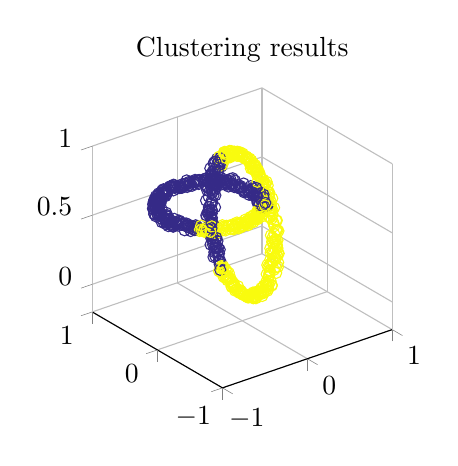
\begin{tikzpicture}

\begin{axis}[%
width=1.5in,
height=1.5in,
scale only axis,
colormap={mymap}{[1pt] rgb(0pt)=(0.2081,0.1663,0.5292); rgb(1pt)=(0.211624,0.189781,0.577676); rgb(2pt)=(0.212252,0.213771,0.626971); rgb(3pt)=(0.2081,0.2386,0.677086); rgb(4pt)=(0.195905,0.264457,0.7279); rgb(5pt)=(0.170729,0.291938,0.779248); rgb(6pt)=(0.125271,0.324243,0.830271); rgb(7pt)=(0.0591333,0.359833,0.868333); rgb(8pt)=(0.0116952,0.38751,0.881957); rgb(9pt)=(0.00595714,0.408614,0.882843); rgb(10pt)=(0.0165143,0.4266,0.878633); rgb(11pt)=(0.0328524,0.443043,0.871957); rgb(12pt)=(0.0498143,0.458571,0.864057); rgb(13pt)=(0.0629333,0.47369,0.855438); rgb(14pt)=(0.0722667,0.488667,0.8467); rgb(15pt)=(0.0779429,0.503986,0.838371); rgb(16pt)=(0.0793476,0.520024,0.831181); rgb(17pt)=(0.0749429,0.537543,0.826271); rgb(18pt)=(0.0640571,0.556986,0.823957); rgb(19pt)=(0.0487714,0.577224,0.822829); rgb(20pt)=(0.0343429,0.596581,0.819852); rgb(21pt)=(0.0265,0.6137,0.8135); rgb(22pt)=(0.0238905,0.628662,0.803762); rgb(23pt)=(0.0230905,0.641786,0.791267); rgb(24pt)=(0.0227714,0.653486,0.776757); rgb(25pt)=(0.0266619,0.664195,0.760719); rgb(26pt)=(0.0383714,0.674271,0.743552); rgb(27pt)=(0.0589714,0.683757,0.725386); rgb(28pt)=(0.0843,0.692833,0.706167); rgb(29pt)=(0.113295,0.7015,0.685857); rgb(30pt)=(0.145271,0.709757,0.664629); rgb(31pt)=(0.180133,0.717657,0.642433); rgb(32pt)=(0.217829,0.725043,0.619262); rgb(33pt)=(0.258643,0.731714,0.595429); rgb(34pt)=(0.302171,0.737605,0.571186); rgb(35pt)=(0.348167,0.742433,0.547267); rgb(36pt)=(0.395257,0.7459,0.524443); rgb(37pt)=(0.44201,0.748081,0.503314); rgb(38pt)=(0.487124,0.749062,0.483976); rgb(39pt)=(0.530029,0.749114,0.466114); rgb(40pt)=(0.570857,0.748519,0.44939); rgb(41pt)=(0.609852,0.747314,0.433686); rgb(42pt)=(0.6473,0.7456,0.4188); rgb(43pt)=(0.683419,0.743476,0.404433); rgb(44pt)=(0.71841,0.741133,0.390476); rgb(45pt)=(0.752486,0.7384,0.376814); rgb(46pt)=(0.785843,0.735567,0.363271); rgb(47pt)=(0.818505,0.732733,0.34979); rgb(48pt)=(0.850657,0.7299,0.336029); rgb(49pt)=(0.882433,0.727433,0.3217); rgb(50pt)=(0.913933,0.725786,0.306276); rgb(51pt)=(0.944957,0.726114,0.288643); rgb(52pt)=(0.973895,0.731395,0.266648); rgb(53pt)=(0.993771,0.745457,0.240348); rgb(54pt)=(0.999043,0.765314,0.216414); rgb(55pt)=(0.995533,0.786057,0.196652); rgb(56pt)=(0.988,0.8066,0.179367); rgb(57pt)=(0.978857,0.827143,0.163314); rgb(58pt)=(0.9697,0.848138,0.147452); rgb(59pt)=(0.962586,0.870514,0.1309); rgb(60pt)=(0.958871,0.8949,0.113243); rgb(61pt)=(0.959824,0.921833,0.0948381); rgb(62pt)=(0.9661,0.951443,0.0755333); rgb(63pt)=(0.9763,0.9831,0.0538)},
xmin=-1,
xmax=1,
tick align=outside,
xmajorgrids,
ymin=-1,
ymax=1,
ymajorgrids,
zmin=-0.2,
zmax=1,
zmajorgrids,
view={-37.5}{30},
title={Clustering results},
axis x line*=bottom,
axis y line*=left,
axis z line*=left
]
\addplot3[scatter,only marks,scatter src=explicit,scatter/use mapped color={mark=o,mark options={},draw=mapped color}] plot table[row sep=crcr,meta index=3]{%
0.0043593806826968	0.478961425067741	0.299026881832958	-1\\
0.0199926698626982	0.00048971550127311	0.505865951731258	1\\
-0.0117227011224565	-0.24360672100125	0.958414698756155	1\\
0.0882904678863488	-0.000557528348384452	0.505375932011454	1\\
0.0210100038552256	0.348999767701628	0.815049966302943	-1\\
-0.463608127682226	0.264759850268991	0.510452179227612	-1\\
0.40707403230632	0.760284014950369	0.522537174485052	-1\\
-0.174482411984346	0.950715838845502	0.477521216667528	-1\\
-0.0163964345826923	-0.102996287482609	0.00111279356299978	1\\
0.0162430734920251	-0.519881728675162	0.595467858161623	1\\
-0.226901485789117	0.0346236077046749	0.487372126649171	1\\
-0.00884220109901114	-0.111583147493401	0.0174786101540353	1\\
0.522727192314501	0.539609608478908	0.489092942254664	-1\\
0.349401590286988	0.191853915938968	0.511412768915775	-1\\
0.00536985617431306	-0.47088208477969	0.356200408896973	1\\
0.342510486230874	0.185292234452249	0.518909965871659	-1\\
0.0627032775522165	0.998029354161384	0.501849030361628	-1\\
-0.0170851413897623	-0.457658207955485	0.217953026010202	1\\
-0.0217322253898427	-0.326144193283837	0.110620185669212	1\\
0.00554254243800529	0.432767743320966	0.203032333357566	-1\\
-0.480660264526946	0.671480874592356	0.521797163867796	-1\\
-0.245175390675885	0.920483804148603	0.484521978307965	-1\\
-0.00726124955064918	-0.073119684416329	0.000212604047954848	1\\
-0.507543424082448	0.348425170102414	0.509310161556645	-1\\
0.474615092497775	0.673565667574651	0.495471749685025	-1\\
0.0247121269078962	0.524192071050271	0.63574591403326	-1\\
-0.262172763770091	0.0636983020345958	0.475516255325265	1\\
0.0158602207050685	0.1503407601216	0.954416584395389	1\\
-0.0249097513923787	0.485015079917175	0.466731935369067	-1\\
0.299984276053998	0.866335601469739	0.480722422586126	-1\\
-0.0218607426611468	0.428112831138712	0.76563707362833	-1\\
-0.00575153892260148	-0.355870147332951	0.895890425838045	1\\
-0.00745279336133942	0.454244091627237	0.476310544341506	-1\\
-0.281020979655332	0.0962329121441635	0.478038882930814	1\\
0.0221865895582375	-0.433164821365431	0.800246032255445	1\\
0.00923953379788209	0.398921830947384	0.21138282373047	-1\\
0.012599143096977	-0.0702122043381784	0.983215411741604	1\\
0.464633524819806	0.580539080068372	0.483555733702258	-1\\
0.402570756483139	0.223323893842404	0.505689129474145	-1\\
-0.513781100007374	0.473093372831973	0.512718495453155	-1\\
0.260121498453634	0.0590124170012024	0.500100919483129	1\\
0.0236146833283658	0.261989442329416	0.041116029637654	1\\
0.425158738648267	0.787556980981965	0.47886413843082	-1\\
0.0083462798815208	0.0199864261990984	0.000699597955272574	1\\
-0.00129368850416921	-0.182228395377656	0.941450251716102	1\\
0.388593784159521	0.825913362013532	0.477973267108167	-1\\
0.446832099773703	0.764944945276155	0.522518395650715	-1\\
-0.0216689010221755	-0.351255734757206	0.903632123732661	1\\
0.0128972129356735	-0.417969056153557	0.778327692435339	1\\
0.000186528764361599	-0.415359646655664	0.259136694525867	1\\
-0.0164203956758051	0.451884166981728	0.414382641775743	-1\\
0.0106645687458732	-0.415993350568527	0.701145685036631	1\\
0.312993850257902	0.110675267782329	0.487697461514205	1\\
0.398439979409278	0.746280111817034	0.504846968733575	-1\\
-0.18355493879314	0.968749827248661	0.524949464069623	-1\\
-0.020017527798034	-0.0415260454784718	0.00213050118778363	1\\
0.00886279533639306	0.350506755563231	0.842077007661243	-1\\
-0.0192866927792378	-0.092915801153639	0.00500500283887088	1\\
0.0239600765559549	0.177241243944529	0.0252414263865691	1\\
-0.0184604639756163	-0.156225150990856	0.948495502389488	1\\
-0.00632407265080294	0.281082555298928	0.118546905380773	1\\
0.248162179756678	0.0935121827552815	0.494408193730443	1\\
-0.00212383649304588	-0.524058518928389	0.601175905391472	1\\
0.00656072303117057	0.436727738701295	0.705351163030866	-1\\
0.495115810297701	0.374811860123211	0.498317443797658	-1\\
-0.00951059640958853	0.242656018128777	0.951396033190465	1\\
0.172756407338189	0.971604870710907	0.483868300981743	-1\\
0.00774134498703324	-0.521971679870426	0.667909639147961	1\\
-0.00579243384541788	-0.548233802576328	0.534048594299953	1\\
-0.0315591833374618	-0.00133479850755233	0.480421081874389	1\\
0.00446308394292638	-0.51315447957226	0.393483890425386	1\\
0.274013739325898	0.110673678920507	0.518225106729547	1\\
-0.328034176192459	0.159105600447764	0.488300496147565	1\\
0.4828611534862	0.66879110828708	0.484236404092475	-1\\
-0.295145541573981	0.113112283827171	0.484846363533378	1\\
-0.0233520299907171	0.0799090413040815	0.000950489373494505	1\\
0.484978346369727	0.304914956003247	0.47735337095752	-1\\
0.0218847908027715	-0.152017967648637	0.0131644294560097	1\\
0.00171786493326392	0.370890410095867	0.227234063387485	-1\\
-0.00827033513098351	-0.37708052004472	0.18442372969839	1\\
0.00915135027621706	-0.120934910851504	0.0217431830876567	1\\
-0.00732515625835103	0.108761446690643	0.0149071475626851	1\\
0.0113289141411178	0.517840677243285	0.356681510659728	-1\\
0.533749670340584	0.468735598227532	0.477706376758605	-1\\
-0.451671919003914	0.775112745212515	0.492153605030587	-1\\
0.409096891664604	0.764893970122845	0.504005575989825	-1\\
-0.0138032799890596	-0.510271046611822	0.627128291483398	1\\
0.412323619299885	0.732539010773118	0.524541877762626	-1\\
-0.0126472412203647	-0.394969781937273	0.849395488722782	1\\
-0.0129212719311495	0.270815786873869	0.0467697444733335	1\\
0.01383262301422	-0.148887379037881	0.971105393052478	1\\
0.478626035423362	0.728396489058849	0.475733145445644	-1\\
0.518040940391632	0.602560834165858	0.476167965927257	-1\\
-0.00543710439327398	0.0282694639883208	0.00275639047190547	1\\
0.0341613025991171	0.997567723895325	0.486236125456905	-1\\
-0.0115366905387746	0.147710204346335	0.00672411328355887	1\\
0.0220767127075811	0.535886058588978	0.453691021498569	-1\\
0.0241787068643753	-0.343542044883354	0.894788278803597	1\\
0.0222701047404088	-0.38816179114838	0.827548765026577	1\\
0.00830394033756908	0.398884670164236	0.860527534916273	-1\\
-0.0144641292992512	-0.0707571423566049	0.996723274552155	1\\
-0.031391176755662	0.998134509367419	0.512573671715764	-1\\
0.0225306313859588	-0.519329158314513	0.328257450758788	1\\
-0.0210304781638873	0.393936963537182	0.71825378128803	-1\\
0.00699511323101332	-0.366453966547262	0.236971832317637	1\\
-0.0100506574873522	0.00995848335936893	0.000908446967237394	1\\
-0.166806334770739	0.957481708960037	0.481316057359473	-1\\
0.289863204637977	0.122194286506596	0.481938111521198	1\\
-0.0902562819549997	0.0148183786686413	0.484060422095125	1\\
0.481231752490138	0.461661250794602	0.493398617958296	-1\\
-0.422482489771265	0.193297001923687	0.516733605160018	-1\\
-0.111233395066662	0.985611872671711	0.497271556467245	-1\\
0.329112579881509	0.149835344291471	0.477627411595447	1\\
-0.400356861743489	0.173662149488901	0.509777958849473	-1\\
0.194792442483036	0.0390564636142438	0.50434002502739	1\\
0.01176647567749	-0.352597830508284	0.119815752242998	1\\
0.0176734170312958	0.494138280119794	0.270490275485369	-1\\
0.10364468266261	0.979984158081189	0.477074159432863	-1\\
0.00482974262026724	-0.483379717600226	0.74958706432558	1\\
-0.0212940512799539	-0.153078112313561	0.986535215950542	1\\
0.264263168220065	0.90757471673381	0.522985183776819	-1\\
0.330811558543946	0.892250088128073	0.506647940278537	-1\\
-0.389181888608762	0.157287279371152	0.512947571138043	1\\
-0.0160650962985051	-0.405510091930576	0.31828168293552	1\\
0.0114009292828283	-0.460924789984008	0.635805837474732	1\\
-0.0223469815367072	0.438903782595794	0.461023919091176	-1\\
-0.313179312552607	0.858045853591608	0.492435772007795	-1\\
-0.509466526078424	0.343365093537333	0.520624295878456	-1\\
-0.000989800740766597	0.190400623444663	0.977361825254692	1\\
-0.0151207321556844	-0.312191684051552	0.125541896541174	1\\
-0.0162117116611346	0.237027781446706	0.0708981655423186	1\\
-0.414624970555825	0.762812360085506	0.491071499391975	-1\\
-0.00899787182566891	0.0196992751635632	0.991053608120946	1\\
0.244467427880741	0.0795367013808713	0.492418624428554	1\\
0.0299876963830273	0.000684176904963964	0.49142554914333	1\\
-0.439381862245734	0.760108199565904	0.495022370782328	-1\\
-0.00827256539503591	-0.366370839954083	0.827623909424848	1\\
0.0208456151650465	-0.184585182614066	0.0527911221889929	1\\
0.414604409430035	0.808528301264059	0.489466206022538	-1\\
-0.00377818677816974	-0.435409790820738	0.444514242092133	1\\
-0.0246479449055562	0.461162832518731	0.702817907597918	-1\\
-0.522547298751674	0.484490608316665	0.475765803402289	-1\\
-0.373861205682992	0.828884557291946	0.507279353461388	-1\\
-0.0224698203136124	-0.300308288247752	0.844605342618185	1\\
0.0898305515237768	0.00293694039322895	0.520467704549281	1\\
-0.00344327898558664	-0.441773568990437	0.415478025603549	1\\
0.000406830885557952	-0.502082657313306	0.505667711254073	1\\
-0.281519392865476	0.0994280922147489	0.496026771750178	1\\
-0.436723305157612	0.25734667588341	0.498588606367124	-1\\
0.0215685685843584	-0.170995463646285	0.0213315639320423	1\\
-0.000967993782848217	0.123990894949608	0.0320043844014122	1\\
0.0169412097963773	-0.0814377532093431	-0.00323930451919333	1\\
0.407100673770943	0.198431421150218	0.48259478770827	-1\\
0.291042356265049	0.0914063374631162	0.502126850873119	1\\
0.0375829924295263	0.995025654721195	0.483838136170475	-1\\
0.0922177879070745	0.979079862439979	0.505549720724592	-1\\
-0.00510167411389366	-0.13643194312656	0.98761072234213	1\\
-0.195492939291588	0.973660012133807	0.518228231384963	-1\\
-0.0140798911840784	0.493440048319496	0.491040924132826	-1\\
-0.00531150623308733	0.205701824546212	0.935202703700421	1\\
0.00888804007294856	0.452765781307598	0.582705633871125	-1\\
0.310622563597491	0.857590983809473	0.485258748067819	-1\\
-0.00740591258991013	-0.161676886454882	0.0159527669707832	1\\
0.00595766039770703	-0.406259843063056	0.823289946722195	1\\
-0.0249667206033395	0.3247602877132	0.0757917947338345	1\\
0.00171550556902487	-0.421069701824592	0.661703692407998	1\\
0.323456165456817	0.135738652771862	0.47860589669355	1\\
0.274173347591385	0.94279654781676	0.49770888901899	-1\\
-0.310663476068535	0.859648032186165	0.522183185962358	-1\\
0.353250271509765	0.140561291514195	0.510509029090859	1\\
-0.00523414531597707	-0.060357083226127	0.991255936196956	1\\
-0.219662704387665	0.938622135458219	0.520344567578314	-1\\
-0.0713385711963469	0.00525027101741679	0.511607947382665	1\\
-0.458508725525188	0.612811514234453	0.475678582063154	-1\\
-0.00359413092750126	-0.250385511841813	0.958151488278269	1\\
0.34115440447378	0.145587317228142	0.504375961610209	1\\
0.00934063665341209	-0.276997416193832	0.0824330401637526	1\\
-0.0171857891902725	0.307476057899291	0.102285668937684	1\\
-0.00456853552587765	0.999931283808849	0.481814523793589	-1\\
-0.0182676883403918	0.196717915884119	0.0641130833180648	1\\
0.0124601724725528	0.337507722894605	0.83367777225824	-1\\
-0.0151428744418778	-0.221112117741357	0.958821033891795	1\\
0.0787334285565358	0.989585837511091	0.493609340457226	-1\\
-0.0109880116650821	-0.451431707935939	0.764802692232066	1\\
0.349316022525647	0.851242592751898	0.515838876595851	-1\\
0.0383856356029642	0.000970592473503955	0.496169116048806	1\\
0.0106377161162669	0.497446746294162	0.685325402754416	-1\\
-0.00673799788748267	-0.381979948595918	0.150793166816892	1\\
-0.246864301017331	0.913532633703051	0.482656920867406	-1\\
-0.282890365230488	0.896050588681844	0.514089315638486	-1\\
0.00457215971982975	0.175686050533297	0.979289984339855	1\\
0.441821752602733	0.375353056245478	0.520358806661705	-1\\
-0.0205433832160966	-0.556537882387065	0.496328368054505	1\\
0.44531506866573	0.33351473346135	0.476379090387431	-1\\
0.330364797628189	0.12229569051131	0.503386888620275	1\\
-0.00732537358226756	0.507351779902618	0.56155515164047	-1\\
-0.0152880876207774	0.0307691298137865	0.993214514267982	1\\
-0.0172388076606477	0.0253140478513819	0.998780981626941	1\\
-0.474088678779437	0.682962944462954	0.480544687955642	-1\\
-0.000517226413154986	-0.202981388232421	0.0596840323984507	1\\
-0.456088091781295	0.777596575680322	0.494744539289441	-1\\
-0.432725884234301	0.295585488764406	0.514822269798909	-1\\
0.465972186563024	0.718626774883499	0.519169214557281	-1\\
-0.0194882566270019	0.0481272544595166	0.00502083955202722	1\\
-0.49376283102292	0.610654560032904	0.511527730598746	-1\\
0.0049145543606787	0.432231371614402	0.660675560601987	-1\\
-0.0133867694000486	-0.316521622629659	0.865296610943132	1\\
-0.491131835359482	0.656780028015917	0.48952209628946	-1\\
0.011160862010216	-0.411306082484556	0.268074333859679	1\\
0.012138816256518	0.221282139208653	0.0824836369269479	1\\
0.00173504896289123	-0.34764217336037	0.884089872850211	1\\
-0.261274692532713	0.0990381526266023	0.507748900730731	1\\
0.0215994127730887	0.4405738362564	0.582133923627273	-1\\
-0.0114624779937056	-0.0686617860978832	0.991841750705462	1\\
0.215476783570035	0.967759997076393	0.503601998094778	-1\\
-0.0181450142909751	0.320561776613283	0.866609914955037	1\\
-0.472116520703201	0.428777105461353	0.519555555969733	-1\\
0.0188149476849013	0.0499790633303956	-0.00010290579879529	1\\
0.0023047109473993	-0.472502817242981	0.494520485950098	1\\
0.0683216036991119	0.00210442884834148	0.510596695039691	1\\
-0.0208782787307547	-0.435162763545305	0.242689170591841	1\\
-0.0222666113896015	-0.0356032531329716	0.999289212082244	1\\
-0.509743415954545	0.517623890911976	0.492673495881251	-1\\
-0.318628121730094	0.108169013219366	0.516904260016125	1\\
-0.016793796224634	0.104092830781316	0.983156646099565	1\\
0.481219472774268	0.339881398187237	0.485340294509798	-1\\
0.318058103159603	0.876091262817486	0.502624984819671	-1\\
-0.282875331216132	0.0591973114090647	0.475790513539246	1\\
-0.0177578328516704	0.304860643573809	0.071154899712771	1\\
0.0376150271068693	0.992978811676176	0.483905214651178	-1\\
-0.0152470130448856	0.535789047529907	0.526642519831771	-1\\
-0.0923241207533068	0.01160400295452	0.477612275987376	1\\
0.224412016865696	0.0735430634371788	0.511953496379139	1\\
0.209279510970648	0.940556464531694	0.486992917292828	-1\\
0.00293993828537858	0.164565958518995	0.946637240924216	1\\
0.00627027730293188	0.502904792205354	0.412795153748148	-1\\
-0.00268580146950436	-0.435785661111667	0.714486139550275	1\\
-0.425408650662683	0.688628132785458	0.477158790845006	-1\\
-0.0038760039939063	0.406876938909867	0.697568091381231	-1\\
-0.0177274524123015	-0.138667814837919	0.0261933923517655	1\\
0.0146448694154273	-0.502240620523102	0.280938200156901	1\\
0.0144710072725092	0.365460333537105	0.104794921655628	-1\\
0.13157172015602	0.989343997394985	0.479310444832281	-1\\
0.508810802389621	0.405493078057688	0.482845180001462	-1\\
0.378203112121713	0.148481411552149	0.484164312788522	1\\
-0.0197190860970908	-0.434902917889584	0.18708073552374	1\\
0.00283423719127724	0.360205279357217	0.187979999782576	-1\\
-0.0335313903246702	0.999221307318621	0.500760089500535	-1\\
0.0153497693686293	-0.0650326522901391	0.991913626266075	1\\
0.00592427125021821	0.531504365680034	0.426772197347968	-1\\
0.346916465368262	0.825787564440974	0.502848032799468	-1\\
0.0782953171918924	0.00222878401084895	0.488751659341356	1\\
-0.335914779247551	0.904012700553332	0.491654289802169	-1\\
0.0158516118224664	-0.527567779459346	0.433465659487805	1\\
0.0223611969840765	0.490709493115726	0.586005902138063	-1\\
0.345696488129988	0.896017672567819	0.483047442556072	-1\\
0.45068852844449	0.558103584900853	0.481235645572958	-1\\
0.185666397365567	0.0246430493433864	0.49796264400776	1\\
0.420429107709393	0.668248097921049	0.508681536416795	-1\\
-0.00705862519371952	0.290567808227417	0.856464685272497	1\\
0.390215887113671	0.861532898419356	0.496879794607897	-1\\
0.15777743019768	0.975737201033196	0.475390490953508	-1\\
-0.00808685786885248	-0.17009376124215	0.0149766310183415	1\\
0.486610818893923	0.643305606430475	0.475040423512893	-1\\
-0.019528092027505	0.069093262130652	0.0108684415546305	1\\
-0.00110455071502717	0.440942263984962	0.278125201095129	-1\\
0.00679420081268105	-0.411709957442777	0.729624980958413	1\\
-0.00639145913269453	0.202731836222209	0.929756048441095	1\\
0.409362536170305	0.701825584950349	0.512688294413921	-1\\
0.023093215244553	0.388125997270629	0.791964508906798	-1\\
-0.315830111722709	0.913971011532953	0.51671512107479	-1\\
-0.158935223956579	0.0336675061987233	0.511808934962959	1\\
0.0222521982879993	-0.2677323909185	0.893957653406167	1\\
-0.00158704090879117	-0.000133583180892236	0.486655980778723	1\\
-0.0128925120927756	0.390266806455	0.278461248372814	-1\\
-0.544929878740073	0.446369750531166	0.5035297456242	-1\\
0.00729389577131227	0.441706740758385	0.631611886062196	-1\\
-0.018403963345106	0.40683678452372	0.837915891398308	-1\\
0.386560743138598	0.196264663565518	0.522414190127875	-1\\
-0.130932484588841	0.0085782442046175	0.489323748723826	1\\
-0.0077718762460584	0.475013875426296	0.435176109985798	-1\\
-0.538863839098416	0.432920561633081	0.479645436163536	-1\\
0.494746568809445	0.623063215457125	0.518047329862936	-1\\
-0.0118748616378739	-0.552043880530063	0.427826965152536	1\\
-0.298713728459723	0.859532188483258	0.493046273529294	-1\\
-0.0168488600354314	-0.137814140702026	0.976307280507641	1\\
-0.19562665571718	0.042687918133734	0.510757682053917	1\\
0.0225934323571688	-0.501635167406495	0.406138518114136	1\\
0.191694528360174	0.973832011609522	0.511776343796967	-1\\
-0.0084491021130095	-0.436603288609899	0.319419021967432	1\\
0.0214765525858876	-0.512516945020772	0.462092917060716	1\\
0.0234771435134911	-0.292380388899027	0.896549105736808	1\\
-0.167300498678857	0.980038286218673	0.513229754685835	-1\\
0.000112048089121231	0.28746701696396	0.919677710310691	1\\
-0.251888883474787	0.0586170487227165	0.517888982524168	1\\
0.0119048955447633	-0.545396178589708	0.434441310941579	1\\
0.0165153659440764	0.396595667974812	0.753245165456793	-1\\
0.0124504623909153	0.136757137874161	0.0182226719327805	1\\
-0.392969992730278	0.143403222783483	0.492910411738824	1\\
-0.0104688234738318	0.485221448143558	0.468213983162948	-1\\
-0.0100939341224589	-0.526810187018743	0.518266174714338	1\\
0.335727437026755	0.154187255886173	0.476370909614509	1\\
-0.0631400023710319	-0.000642596759899103	0.524875710428062	1\\
0.0158387786541794	0.2085872683017	0.92196433772386	1\\
0.014729119330426	-0.504675411122612	0.592199821955066	1\\
0.00388228948744707	0.443583026992268	0.727545310777846	-1\\
-0.0141216104998871	0.453732836162598	0.546560412966627	-1\\
-0.0111770416089134	0.455000853645252	0.477244558704465	-1\\
-0.0139756844784457	-0.507931895207694	0.43393947242188	1\\
-0.0531147324092611	-0.00219908365869111	0.506508500820622	1\\
-0.324340140252556	0.14125397490796	0.486682915981155	1\\
-0.00609435435979653	0.219370007531633	0.929566804556931	1\\
-0.464415690974686	0.223740318955516	0.524327745957354	-1\\
0.015535220214854	-0.17819231339088	0.97294207483793	1\\
0.0129811428621377	-0.0914098518755163	0.00316540025965508	1\\
0.487367641284123	0.65844332163414	0.490858249075762	-1\\
-0.501725135949098	0.442892621889336	0.494839211375669	-1\\
0.00437740451482965	0.467549933683599	0.344962196904348	-1\\
0.116876089723616	0.0171720343771697	0.480740374222773	1\\
-0.0220045002641379	-0.391217695376096	0.175597923772497	1\\
-0.327496498629783	0.861202766999163	0.494735602311061	-1\\
-0.0131602654424717	-0.000806017530978467	0.510183420162529	1\\
0.535341145848858	0.517593695557787	0.512015049746199	-1\\
0.446464399395966	0.218081203810897	0.497447007327437	-1\\
0.0482583579401082	0.00354574964466828	0.50782229100549	1\\
-0.00443390532589506	0.145926495890149	0.959736776267248	1\\
0.0244927798244964	0.310538554617753	0.917173235892571	1\\
0.0699213833343257	0.00173264142155635	0.476476082726365	1\\
-0.375190013233378	0.225674315625118	0.508254389089877	-1\\
0.0157652767929712	0.417235540454084	0.654367291428653	-1\\
-0.157711756563664	0.958640510165817	0.501635542592347	-1\\
-0.457953992623491	0.320569380360156	0.507030378439932	-1\\
0.42103639973477	0.715859087036311	0.509692767570455	-1\\
-0.120224846295031	0.987793935698527	0.50631829780767	-1\\
-0.146222623359108	0.98620867893586	0.486103676178575	-1\\
0.0151910608713463	0.999360071445961	0.496514780277496	-1\\
-0.473685484181338	0.501822224504851	0.499607304997959	-1\\
0.00154987644512268	0.321318753442549	0.835320423567231	1\\
-0.520894807657472	0.649105303276286	0.48792725668524	-1\\
-0.00927445785243184	-0.241352100384897	0.921993396565572	1\\
0.0176604059124288	0.487919555206116	0.406879371712654	-1\\
0.0070994594844534	-0.500156466113716	0.383121526591316	1\\
0.0164728918002659	-0.343506676859842	0.117663341752638	1\\
0.347998501134409	0.868489692265228	0.478428334233655	-1\\
-0.447279743047677	0.321240405748184	0.512826949044618	-1\\
-0.0112736532720387	0.488736789612864	0.604133140361712	-1\\
-0.383692188826925	0.75681527135529	0.520730106597509	-1\\
-0.015798295062685	0.388852783992595	0.249065291329362	-1\\
-0.321997673014192	0.0923826786704125	0.517574258151596	1\\
-0.400455150671451	0.806885398426707	0.51727534695152	-1\\
0.0128874565473673	-0.450610935922264	0.52416050423496	1\\
0.00594933572251069	0.300744126648995	0.90601719228229	1\\
-0.501409261772018	0.514568179242656	0.522508105483097	-1\\
-0.475070651131357	0.648037435102557	0.487342600527584	-1\\
0.0239421428052751	0.392866403971725	0.845193969690359	-1\\
-0.426382744995588	0.726442228144266	0.508531547606766	-1\\
0.0105837360556797	-0.519534807191816	0.486084268257683	1\\
0.00879058944613581	0.4957638035601	0.722742049671365	-1\\
-0.438664780696935	0.220476194041925	0.481147518413713	-1\\
-0.00555536143159944	0.116547267452011	0.0192777997500467	1\\
0.00572371956704	0.14469382369827	0.98084318501102	1\\
-0.290291558022365	0.907773909633709	0.51993840885386	-1\\
-0.0192210185376683	-0.181789921440989	0.95934386411463	1\\
-0.372957352290681	0.208701642065911	0.505658621413584	-1\\
-0.408740148219957	0.705398632402873	0.501367139221594	-1\\
-0.266946375440358	0.932025342402598	0.523168562249813	-1\\
-0.0138089351619959	0.11386309495987	0.97294919017985	1\\
-0.273093465242382	0.051386253111599	0.476954446848408	1\\
-0.00779944065716039	-0.535178935413351	0.501332914440227	1\\
-0.0214129365263582	-0.199023696568062	0.0219457281962659	1\\
0.00703484821584447	0.475862661592857	0.719232770714003	-1\\
0.0183795447657495	-0.0897358778800509	0.994827811896439	1\\
0.429491995836666	0.326709922611876	0.486801795021552	-1\\
-0.00308074167816241	-0.423575003894358	0.747230004800323	1\\
0.168696911363485	0.951343635506814	0.513436093262544	-1\\
-0.018459445859875	-0.110419927991375	0.0144483164445947	1\\
-0.0955246515747005	0.989442736482378	0.517337284040021	-1\\
-0.00261782680707695	0.349844786254324	0.891853695454793	1\\
-0.506280100082392	0.412483555399039	0.481916948839158	-1\\
0.216089857201755	0.932857176230501	0.513235185812833	-1\\
-0.420310216934098	0.82061101812486	0.50554090650679	-1\\
0.0123312436743315	-0.258227209773576	0.0727006342058011	1\\
0.523404864952893	0.411314785241895	0.508867926019519	-1\\
0.272765689357211	0.926453713538913	0.515594232696509	-1\\
0.0137816504024931	-0.505841144735098	0.592519168917025	1\\
0.00968017949444031	0.0780333772174981	0.996241371424727	1\\
0.399747638656227	0.849770219781594	0.518691060895577	-1\\
-0.0165478454394477	0.0153432482595085	0.995905805396326	1\\
0.0792251656335928	0.0104752776820626	0.508817281588143	1\\
0.518477245454978	0.451888963866229	0.495219107589617	-1\\
-0.00514266290654378	0.200906425329057	0.969277378645483	1\\
0.0133695313420437	-0.123911862713174	0.990527570857065	1\\
0.423800165981472	0.317993326230099	0.476550355742932	-1\\
0.00903614712395317	0.430321857007354	0.660753491288271	-1\\
-0.043155930977164	0.0011735816843757	0.476883309951684	1\\
0.495451029914429	0.333422662908138	0.489420709762874	-1\\
0.00776252463242632	0.374975974189633	0.840936788356882	-1\\
0.0232624979765357	-0.298158577468723	0.0775967462658513	1\\
-0.182039722427426	0.970682915009582	0.498435900386578	-1\\
-0.00848948382054872	-0.453292828436832	0.338868804216974	1\\
-0.00567651947247809	0.461698800399636	0.389295350745044	-1\\
0.0103252871025935	0.41993286147724	0.209341441187674	-1\\
-0.0179994221444796	-0.175567193996453	0.955531677277937	1\\
-0.00136140316889287	0.253574087065363	0.937458988067022	1\\
0.383303143525145	0.840744490013217	0.509789114424787	-1\\
-0.504262984105033	0.608751036775588	0.481779598592793	-1\\
0.000875526145199901	0.0764685679910257	0.993800133053634	1\\
0.441765426031914	0.631570841481208	0.493442747483033	-1\\
-0.00235145526907266	0.265355536888144	0.923006051173048	1\\
0.00678593468594751	0.277749486698172	0.945214517349246	1\\
0.388891626009524	0.146079585966985	0.503311836970499	1\\
-0.455118682894251	0.352191563912925	0.511939256839659	-1\\
0.0178682094672773	0.0978488547617722	0.993344834372625	1\\
0.469635789636471	0.504038671756185	0.489260001689212	-1\\
0.0175028825279168	-0.047243001133217	0.986222948230102	1\\
0.290465209416042	0.931485927498331	0.497775443610592	-1\\
-0.0212269169345885	0.496861820572592	0.629065068875867	-1\\
0.00516151555217386	0.551514125189842	0.398591378513723	-1\\
-0.0161500717913755	-0.45181318144708	0.369435507860902	1\\
-0.223830838283066	0.935302873111749	0.516323443114807	-1\\
-0.0215797764381246	-0.000695328473043609	0.515633909556023	1\\
-0.020425627936579	-0.433640411468426	0.207717068692045	1\\
-0.00487912068747145	0.47616669023305	0.725043678279061	-1\\
0.27281593502893	0.940832820781544	0.509797553575325	-1\\
0.00488422681716484	-0.456078883470515	0.499829295594925	1\\
-0.0158082062952995	0.469999024250261	0.777634713388989	-1\\
-0.0221203284243254	0.439921000245658	0.631619527065537	-1\\
0.0119339427780986	-0.490801369751841	0.454968132968527	1\\
-0.0241485259856376	-0.350722786158013	0.888881573152575	1\\
0.0206210833363732	-0.427514801159874	0.72677139652449	1\\
0.407941593589588	0.807183414421151	0.508556393010679	-1\\
0.510940275786233	0.404755851870785	0.499658999060897	-1\\
0.0188605651363015	-0.188864623858131	0.0243092262918549	1\\
-0.101086658930327	0.00819117420265325	0.517788108515566	1\\
0.432437889347285	0.182112380149897	0.497928697434421	-1\\
-0.0100697353390251	-0.318174348985302	0.865348603266272	1\\
0.0117462367134899	0.192276237886026	0.049993513008727	1\\
-0.195526693147743	0.049885560408639	0.519116425332579	1\\
0.499618886568163	0.484752760325463	0.520056998056694	-1\\
0.104105447865323	0.989300326425113	0.522319182445618	-1\\
-0.399060029360598	0.252118870529633	0.499288434187204	-1\\
-0.00213791217594918	0.492951494156215	0.375596298861162	-1\\
-0.0108758922212684	0.39792662646778	0.846154668335921	-1\\
0.463691501528025	0.572666006856834	0.482847428989742	-1\\
0.382068113395867	0.767453916264634	0.494068493410195	-1\\
0.0163123331582677	0.357486674995793	0.87562015212946	-1\\
-0.141916445850961	0.973698139077214	0.482058287829502	-1\\
-0.382738752671683	0.80643098079869	0.509925097686464	-1\\
-0.321249367273474	0.128208922973481	0.49937706389439	1\\
0.0122584076387706	-0.156573807021287	0.0370180551243291	1\\
0.00156335725231385	-0.446290325795119	0.659804135073725	1\\
-0.317796472101205	0.0772674203627145	0.496138419912701	1\\
-0.0230932608803687	-0.240428186454274	0.962077638991801	1\\
-0.407560703110568	0.271237415928795	0.482505032657593	-1\\
-0.00937418849487281	-0.0722700521260137	0.992612386766726	1\\
-0.0330664695405201	0.00273294764595333	0.486713331583788	1\\
-0.499277513505764	0.386289441478959	0.511794411402502	-1\\
-0.0211248003194081	0.326714756067945	0.151496391749615	-1\\
0.216196161940464	0.963133339150798	0.485936736600499	-1\\
0.183399680032625	0.950792036097097	0.503204133840828	-1\\
-0.387300875207209	0.771445683592876	0.488481600376413	-1\\
-0.0076468011696646	0.439188289263068	0.232386570089131	-1\\
-0.0237934795645883	-0.0222299801805556	0.997467562984284	1\\
-0.00449400151679002	-0.406861346335422	0.304649742296994	1\\
0.010939744395211	-0.363653140133604	0.143343308338621	1\\
-0.0166508865763025	-0.24045254828634	0.944067945702998	1\\
-0.0139690775890095	-0.504320785122036	0.309496161616563	1\\
0.512479190418318	0.530949892039179	0.482307596782023	-1\\
-0.0212348675766714	-0.0328847806773336	0.00441039799942569	1\\
-0.355242554082385	0.143503719906681	0.495484627666378	1\\
-0.0130574420010431	-0.020657118168989	0.999728326759533	1\\
0.376978997286385	0.19515471221735	0.480214011332345	-1\\
-0.457892886820382	0.572787297529019	0.52175136039094	-1\\
0.0230860368233311	-0.381187303219442	0.791741472454552	1\\
0.0155693033075756	0.0599053582286482	0.00265143896105501	1\\
0.0446634453407604	0.998925271313073	0.477818925437719	-1\\
-0.352320995221312	0.798893682682456	0.507850129485528	-1\\
-0.154459647128026	0.9863198559236	0.481696978993703	-1\\
-0.509520259879914	0.613546172065784	0.517205288922591	-1\\
-0.299822289799602	0.104733432288906	0.48489393760973	1\\
-0.000405454732756552	-0.507790311660209	0.387889148860568	1\\
-0.0515689507485599	-0.000290398641698081	0.509599822489119	1\\
-0.0110908580614199	-0.22867459472961	0.0332396445616851	1\\
-0.533088563808675	0.513352713674409	0.485986815103356	-1\\
-0.00457329823529926	0.36028881790397	0.17053258940611	-1\\
0.0214539851943225	-0.433783756300526	0.350489345648787	1\\
-0.0218267121803668	0.0515655621978446	0.995273024622334	1\\
0.000165991457901765	0.552006237212377	0.412191547234831	-1\\
0.00306809427783621	-0.240992266006617	0.950138276661664	1\\
-0.0161611289890546	-0.400999666641078	0.802500191626957	1\\
-0.185054204792877	0.0448968363747178	0.498951579574113	1\\
-0.543851640560439	0.45871529818741	0.499209312701538	-1\\
-0.475444111091006	0.738993380598972	0.501095136833354	-1\\
-0.465177715192763	0.695707754253198	0.504197771205556	-1\\
0.107425090281239	0.0128855389509286	0.524767071023351	1\\
0.0406633331139483	0.99834016056557	0.48245201146968	-1\\
0.497861328644562	0.463871765415462	0.49813757274546	-1\\
0.000129458922278458	0.417890122583691	0.781132216810128	-1\\
-0.468296867262678	0.372648562831454	0.484721090280262	-1\\
0.42338467463001	0.784216791401532	0.50990771141677	-1\\
0.011793059655759	-0.305608678682722	0.0864050508563707	1\\
0.013372042086184	0.0747449007738303	0.996676738235213	1\\
0.0201723210508637	0.281095408332408	0.0912006796005248	1\\
-0.00823459079861083	-0.134944189528827	0.978342398010718	1\\
0.238336663403205	0.0603574555868909	0.517877712728148	1\\
-0.0451127830923892	0.998981582745863	0.478261166014618	-1\\
0.0203930359922376	-0.457609900001608	0.622702282514032	1\\
-0.0116384814533579	0.458349890009099	0.634006979507952	-1\\
-0.39450971267982	0.841677948346444	0.478131058517852	-1\\
0.441396817056941	0.225136617322674	0.509910685746787	-1\\
-0.178868255596047	0.0249230639639852	0.484454907698268	1\\
-0.369154868747491	0.86833678544941	0.51559962764948	-1\\
-0.384660240675413	0.241723273359221	0.48145568329469	-1\\
0.0189673216844963	0.291004358195437	0.93321036988109	1\\
0.00668416681560403	0.526607398543245	0.656321617862072	-1\\
0.00255387297847091	-0.464893600153217	0.427049773009195	1\\
-0.0197282147244407	0.138581325963082	0.0163553336538432	1\\
-0.446754988901948	0.751082971554425	0.522586742603658	-1\\
0.00554106196378661	-0.460751597073642	0.356113677312775	1\\
-0.0150599082703043	-0.206611929508126	0.97339734109683	1\\
0.546952091180883	0.483558290368622	0.515069105983384	-1\\
-0.00857813637356279	-0.399520195660114	0.179109061810484	1\\
0.0236141763234266	0.163600261657576	0.966154626951381	1\\
-0.0152126162678534	0.175984983606077	0.982999079507918	1\\
0.454140690688854	0.258762772337641	0.492160486312875	-1\\
-0.00491804984051065	-0.468259413679759	0.700181174812252	1\\
0.44568912193951	0.603492958586467	0.504013831622808	-1\\
-0.251457061502565	0.0934666801692864	0.497889115776665	1\\
0.0599130695177338	0.00247106738679265	0.486276717587126	1\\
-0.41380693530715	0.190913842002509	0.491204402002334	-1\\
0.123994102326043	0.990983054480796	0.479323495738307	-1\\
0.0130253325191528	0.433570455065131	0.18304476805281	-1\\
-0.463163289580691	0.282101062391909	0.475007456259722	-1\\
-0.0123189595902032	0.240304256629229	0.945669041078539	1\\
0.445246076532693	0.700005223032218	0.480961512311854	-1\\
-0.00797098399865623	-0.00318170940409939	-0.000151237499429228	1\\
0.0222339425017474	0.26455820373648	0.0798836737326158	1\\
0.490163791991992	0.324523390547694	0.489411417877203	-1\\
-0.0122833912711076	0.0968399476132462	0.98913919563265	1\\
0.0138023801846093	-0.271606005048007	0.0655987702294471	1\\
-0.0804350512907256	0.988397338530203	0.519804370526133	-1\\
-0.00283281286486755	0.345295053151175	0.83516584517775	-1\\
-0.270123892625973	0.892638699033501	0.498956664096624	-1\\
-0.270830486488434	0.942067335513253	0.51122812589192	-1\\
-0.0462899655510212	0.995789698703355	0.518049865071235	-1\\
0.131118771861154	0.988075915106548	0.498005052701914	-1\\
-0.403470188124356	0.795454917444359	0.479634168140612	-1\\
-0.356861699598834	0.872889636878367	0.517667547977794	-1\\
-0.490782395331002	0.506872559366888	0.518419108186507	-1\\
-0.00808626159242501	0.0781962010510534	0.00452529706530806	1\\
0.0188034091642813	-0.190398445943662	0.961875242082256	1\\
-0.505410817446914	0.365084440901771	0.520853646130663	-1\\
-0.0725374463909634	0.00921153194115236	0.499524836776668	1\\
0.0109182339146773	-0.445672725689822	0.489206877035014	1\\
0.0185066903670066	0.50693954290865	0.505984204422717	-1\\
-0.298463490917857	0.868200979640417	0.504679943700706	-1\\
0.493857264704415	0.347594094456225	0.479579963576126	-1\\
0.00118741364792045	0.455934516401966	0.383720020827762	-1\\
0.00839766630210372	0.000401259231602739	0.48931473950546	1\\
-0.334360181760132	0.163964366305717	0.479564514119899	1\\
0.000783782977233172	0.284419965638333	0.939439291540602	1\\
0.008881645653089	-0.453026262015175	0.690425999483643	1\\
0.083790255709869	0.990330004008066	0.501680417542427	-1\\
-0.000160781606240235	0.504840571659637	0.319027259635275	-1\\
-0.00646145129349487	-0.448674496902287	0.543033813645528	1\\
0.0800590735677687	0.98540491825913	0.487249615503223	-1\\
0.00943609502823269	-0.454764118078852	0.414957857376139	1\\
0.00821889303131763	0.0659937731788768	0.997664625990281	1\\
0.0221424043493869	0.055672816466033	0.998420057393521	1\\
-0.41708580148539	0.756674776398153	0.500962241767521	-1\\
0.472699814472699	0.290896656652694	0.487013964966523	-1\\
-0.489564633835686	0.467080016678043	0.502895553122932	-1\\
-0.015834391706588	-0.372942827651214	0.820723113649166	1\\
0.00294003990514708	-0.358824514926253	0.785095776423672	1\\
0.0248653773381798	0.449506175658111	0.492604616437143	-1\\
-0.381109155511121	0.152980625811269	0.497224867641127	1\\
-0.0180778748653703	-0.192121322294199	0.0617142964839102	1\\
-0.0134685143753753	-0.281941469264165	0.924561369641165	1\\
0.215855322531842	0.0733500577498862	0.476014037471085	1\\
-0.00292698583560348	0.216745500431979	0.0655008229345998	1\\
-0.0238110517348724	0.999465782867543	0.496873384979194	-1\\
-0.0124067004910065	0.319764245570998	0.147810563506006	-1\\
-0.000988599929687575	0	0	1\\
-0.253856121332303	0.0569121253294356	0.501203023350599	1\\
-0.0161302663036771	0.999101433157523	0.494989291207633	-1\\
0.0179697518200742	-0.431085497589702	0.169444509133851	1\\
-0.0198582150321491	0.512564343126843	0.631603180475447	-1\\
-0.23644918446544	0.0455436047230447	0.502135683235096	1\\
-0.185076266590092	0.0510428032901244	0.481779900954171	1\\
0.00761397503681845	0.0730623933743696	0.980983781586005	1\\
-0.00160734136262755	0.519198561064976	0.323732810967519	-1\\
-0.400354549429377	0.232942874239531	0.482913905263272	-1\\
-0.0232108724320149	-0.361936713159376	0.805092592719584	1\\
0.0103777525036521	-0.0615518105029911	0.000484513411035769	1\\
0.0203008027478428	0.44379257901278	0.621028612147915	-1\\
0.0122480381231756	0.0382147873410891	0.00374554386818716	1\\
-0.528798804014779	0.370078588880022	0.490592278696567	-1\\
-0.501899237565617	0.542425991570102	0.496128794985335	-1\\
-0.00873480206337059	-0.211778023795041	0.968996233412164	1\\
-0.00500495751634546	-0.448109011157003	0.72054657368089	1\\
-0.000102917780956666	-0.243258570474194	0.0597494628293724	1\\
0.508839605886128	0.515435899446998	0.494489414366872	-1\\
-0.437374384154497	0.258942597324141	0.518120887416227	-1\\
-0.527000634946486	0.37473647099712	0.491061617662752	-1\\
0.00714545156040151	0.516914821497938	0.344125941206886	-1\\
0.00537014184213249	-0.429433687138952	0.736949233951632	1\\
-0.521083119491365	0.496241649709949	0.503034943131919	-1\\
0.304828982400548	0.0712904147976316	0.509232226014904	1\\
0.0283369937197632	-0.00194295382000684	0.498116776584414	1\\
0.0244726326062039	0.0250711065431452	0.998475032876945	1\\
-0.0162565721339149	-0.347451447391462	0.784629658656065	1\\
0.0240530496308006	-0.209596456699169	0.0661374443252364	1\\
-0.00241029103004997	-0.270009432685835	0.940193335347282	1\\
0.236480730157101	0.0727020172978582	0.519708813530546	1\\
-0.172360049145152	0.963226557169321	0.507984077572476	-1\\
0.0229560980453466	-0.249777889531842	0.895360646908502	1\\
0.00858020333456009	-0.502037854449347	0.523584283836432	1\\
0.0178140496045297	-0.039973910100057	0.996693701601217	1\\
-0.443355284742512	0.389929173768422	0.511303000757032	-1\\
0.412584005355157	0.83165099523561	0.487126788960584	-1\\
-0.0806649967270442	0.0116515683313402	0.49350201286647	1\\
-0.00077705923387594	0.297051236726149	0.0624340667967979	1\\
-0.000139987711374062	0.242266042584517	0.910267497895644	1\\
-0.0235402693039489	0.130644390830336	0.969098149745705	1\\
0.21115223081577	0.954452652761708	0.509065961510603	-1\\
-0.454282246862549	0.71034724480527	0.475403449368741	-1\\
0.0136041879655432	-0.373992092913548	0.879853354931902	1\\
0.444026554342783	0.304297700210832	0.511956556253337	-1\\
-0.0201274600112654	0.415690435098179	0.151742561273228	-1\\
0.528949629587177	0.416281895594809	0.504095544826443	-1\\
0.00475575914608656	-0.415202043233573	0.277937537333967	1\\
-0.344600700471244	0.114419649861457	0.482080369742428	1\\
0.470240255054822	0.522949370395302	0.497275117979131	-1\\
-0.526596790208803	0.529485035102429	0.520004636504239	-1\\
0.256551650469205	0.0985385714313994	0.515451436118846	1\\
-0.0910136039647885	0.991998211586293	0.518963834263436	-1\\
-0.151464135109467	0.018476484147842	0.512116105548892	1\\
0.449996039057375	0.480325925036146	0.484539559893314	-1\\
-0.0195566961645107	-0.420458218257849	0.787422863706692	1\\
-0.0132114760396992	0.127521752252401	0.023306943927092	1\\
0.146623716818912	0.0288659159460513	0.50105680953126	1\\
-0.479833695525903	0.359800615665878	0.522511875276338	-1\\
0.505424078022213	0.52831877279009	0.522970790718187	-1\\
0.0178360813434397	-0.142870463158897	0.971707329101116	1\\
0.155710102541175	0.0252600076672988	0.492995619736908	1\\
-0.313044924660836	0.90590842563199	0.501772606956786	-1\\
-0.0190286398408644	-0.258279228144128	0.880331893152203	1\\
0.0243849292201437	0.412346595539573	0.258711280110418	-1\\
0.156090592499925	0.0319063926479003	0.521910670558248	1\\
0.0487867606923529	0.998780218806966	0.489639138246983	-1\\
0.358809330607673	0.877993441154307	0.515846341688852	-1\\
0.137749415137685	0.00772522887217969	0.483081213216752	1\\
0.490596568306627	0.31131473615358	0.523756966010293	-1\\
-0.00317103723283549	-0.00030111522933773	0.48099639100226	1\\
-0.0210411117993755	0.232272789660681	0.050516232971223	1\\
0.368270139337644	0.867561090782014	0.499961854380045	-1\\
-0.445574041573537	0.572403950944119	0.501038999599728	-1\\
-0.505592728476442	0.694366226792276	0.488925301315417	-1\\
0.0215092167007853	-0.492801527728159	0.656666618286349	1\\
0.0158932415088208	-0.23751095597024	0.0745858457684234	1\\
0.0204448071708186	0.555569382811347	0.431212943165538	-1\\
-0.295538947100961	0.0815165812734599	0.523184851263703	1\\
0.213349333553297	0.0458936843409033	0.47620842784704	1\\
-0.00941528923461281	0.434535870463919	0.255645102933788	-1\\
-0.0563643195935065	0.997198082197652	0.505638642590806	-1\\
0.527705302956552	0.473852591085587	0.520401651131095	-1\\
0.384758060068754	0.8129522287214	0.511587294188689	-1\\
0.0178712952830454	0.149390684301722	0.00376548550126837	1\\
-0.527763024742615	0.421564583420859	0.492307636395598	-1\\
-0.0104641707294139	0.472525724501669	0.22343092662249	-1\\
-0.000926122162383536	0.225808652695006	0.0313720194648615	1\\
-0.0202857038513214	-0.237014599434988	0.0326239357529515	1\\
0.0397457226972775	0.00440730937890997	0.522507457580835	1\\
0.439390150252401	0.354622924559081	0.511844470557569	-1\\
-0.530797596157364	0.543808468288611	0.476307558520371	-1\\
0.416272739043605	0.754364782684221	0.476717814370067	-1\\
0.00115686801401396	0.464062366808045	0.29150704109743	-1\\
0.177494717016693	0.978963782379872	0.499079728927637	-1\\
-0.405582919569552	0.832247151612451	0.516087849317501	-1\\
-0.0216355225228591	0.400813606624124	0.190888382106483	-1\\
-0.369660338113035	0.864469190029982	0.509600338601737	-1\\
-0.0201190835867165	-0.304257171717703	0.0856320788136164	1\\
0.458418209396981	0.209829899364053	0.478478354325021	-1\\
0.0240453039789437	0.096390523288018	0.019017181524965	1\\
-0.0226065560662668	0.051311815145262	0.984112934556206	1\\
-0.00234182696094238	0.312743335428409	0.111381198337377	1\\
-0.0225051256996181	-0.100266509682433	0.0152392580074298	1\\
-0.39176432516321	0.214827838882464	0.503147249667787	-1\\
0.0175090619975809	-0.372159545485112	0.834159002457559	1\\
-0.0425703199023117	0.998908920838019	0.519607522551435	-1\\
0.219584865099716	0.055239992593756	0.504809520157885	1\\
-0.00367772100445567	-0.496283715727373	0.566817562404918	1\\
0.146999114483435	0.0159617827504373	0.50352392198061	1\\
0.187298350058122	0.0242282949719949	0.493910602491782	1\\
-0.0241072825034766	-0.411222518973883	0.171039802062482	1\\
0.0109542999277477	-0.386475322009279	0.134510453639048	1\\
-0.002333077987953	0.334175595006898	0.0768477589754027	-1\\
0.00925737748317854	0.164517602854793	0.959482209981331	1\\
0.416966964310859	0.691584149762922	0.498433516693657	-1\\
0.435526750707921	0.719992963640182	0.50299285054031	-1\\
0.00376444592417913	0.402584730977453	0.288865333592154	-1\\
0.369084330256097	0.173335928874408	0.510946285440196	1\\
0.13913656135004	0.989366093806526	0.50582032134855	-1\\
-0.00743077021460653	-0.451858006486754	0.742288246185582	1\\
0.000918459143579398	0.515686668165873	0.670638265208071	-1\\
0.422702886149167	0.206908184125364	0.478047112116748	-1\\
-0.334720530392453	0.841650387828159	0.49063948888542	-1\\
0.0200685306190542	-0.141451780239116	0.97405135253318	1\\
0.00111395892404765	0.0032421686839165	0.997601112865739	1\\
0.0194232308249673	0.464740245715061	0.719424092064263	-1\\
0.218354084434508	0.946282550694793	0.513196278162516	-1\\
-0.00639042482757617	0.431833232819749	0.821820539037404	-1\\
-0.00567850622160842	0.466879950323691	0.267917493458106	-1\\
0.00117203207084904	0.0299844838826321	0.000812870647824949	1\\
-0.35891942893614	0.10469290346884	0.510707740835594	1\\
-0.00556909478060325	-0.285396908191375	0.921209154575368	1\\
-0.022494328154539	0.352483010752497	0.20499832733513	-1\\
0.00249953206206102	-0.382668446671539	0.121614499558446	1\\
0.342569828974748	0.894673292795709	0.523785467486081	-1\\
-0.00649536091354558	0.530112301253885	0.6000402021024	-1\\
-0.277646804430144	0.933429943893382	0.505949204237987	-1\\
-0.0151380948727095	0.018327057801709	-0.0017061908587852	1\\
0.0128796858112484	-0.539467182819367	0.595499621764454	1\\
-0.0829852285026614	0.0041594123297963	0.494035003808728	1\\
0.39081068583956	0.841448193801115	0.504399822264761	-1\\
0.00506353957341441	-0.323977205064543	0.14208442069739	1\\
-0.449212131166369	0.407424026329991	0.483058609687018	-1\\
0.449494329677425	0.353039925037282	0.507046279447521	-1\\
-0.360132872462445	0.126370198331403	0.488932269890908	1\\
-0.111481367490334	0.0181164378379434	0.5083364499603	1\\
-0.458127068313809	0.334534302106351	0.499376801097783	-1\\
-0.0100499830582391	0.178331992070014	0.057245013721632	1\\
-0.00578001861100782	-0.422640175207103	0.669160537018854	1\\
0.314575147799708	0.0777583477069129	0.52093046434063	1\\
-0.00467610333142824	0.352287719522402	0.13899035338116	-1\\
0.0161648188031573	-0.39058860742282	0.232021941616447	1\\
0.00767608197247253	0.355106783912833	0.215580876321862	-1\\
-0.0154239256308782	-0.474589438023203	0.732888849158242	1\\
-0.00822477793492223	0.403296588845152	0.159062527724841	-1\\
-0.424841381902409	0.722057824636885	0.510828844183328	-1\\
0.271433877439561	0.0519239315866734	0.493171312183611	1\\
-0.0098478517963905	0.362235309616325	0.787294456370273	-1\\
0.431734116697412	0.224870838013633	0.487701192799851	-1\\
-0.412362039711254	0.74061816670852	0.476990565890132	-1\\
0.000177536253743948	-0.530972638332401	0.485645394982834	1\\
0.0104975330594167	0.299070459811796	0.0975140047675948	1\\
-0.506477682426254	0.435635895099555	0.479628478394484	-1\\
0.014335230368518	0.141469142380125	0.982581072649493	1\\
0.472550539422407	0.426468723404982	0.492697170911771	-1\\
-0.0150882690399284	0.452818136845114	0.348766506457554	-1\\
0.434829276855818	0.33135268360881	0.482380608529107	-1\\
-0.139776816831525	0.019424164107195	0.511901799058998	1\\
-0.00242298607127761	-0.438884673871439	0.760395383309637	1\\
-0.33240077466914	0.875178380836161	0.492851116166984	-1\\
0.257009918873448	0.895301687645055	0.478684157938643	-1\\
0.0116784529299577	-0.179104018989784	0.0231681324027786	1\\
0.399230645936135	0.14845645572398	0.522149064679535	1\\
0.0101152577035988	-0.539270147959559	0.368306843180715	1\\
-0.164559223986932	0.973543972593209	0.495440418651437	-1\\
0.0173069006146476	-0.430884645439851	0.173763078472345	1\\
0.446951415351019	0.635668886386704	0.490583938878123	-1\\
-0.31665760457379	0.0755667299174428	0.489401352477246	1\\
-0.49566724026478	0.538959065750753	0.498671699878575	-1\\
0.415897410863976	0.235667969152324	0.47841392339358	-1\\
-0.500067165080772	0.43162524705067	0.499159116362216	-1\\
-0.0211466310350736	0.208620897668495	0.0640428719375501	1\\
-0.531653469183273	0.569472403147358	0.518016803891111	-1\\
0.0175471113349365	0.481852299581482	0.520410920557043	-1\\
0.509700252624326	0.338490370887519	0.492876668395057	-1\\
-0.0203859105861696	-0.376528777276843	0.742223130378136	1\\
-0.348648033058796	0.176735563536954	0.513711524369038	1\\
-0.0194702113944782	0.273357929085031	0.108214834054972	1\\
0.304465430100499	0.873038991142308	0.52362155856799	-1\\
0.276872896280993	0.0651105617918381	0.476741231844547	1\\
-0.121240250992492	0.00358542259754748	0.514363937237801	1\\
-0.50624369363082	0.687489536939812	0.487799933334246	-1\\
-0.00489237628849288	0.0267489138479462	0.99945773291036	1\\
-0.0155049928112081	-0.121162575197349	0.00562886200507747	1\\
0.00594902671675411	-0.150251737757286	0.0151411529478018	1\\
-0.000374266444898824	0.472562793792868	0.37806744320344	-1\\
0.277443195465818	0.913421838864534	0.50848824784811	-1\\
-0.340819454490219	0.898828190087624	0.485577988242475	-1\\
0.4494941060369	0.231341755219036	0.494542563020467	-1\\
-0.0127158285035678	-0.262773785162224	0.0611716402956098	1\\
-0.00313538945268059	-0.0512220325067857	0.00597866193661168	1\\
-0.282135546123115	0.881144648632089	0.50206955974691	-1\\
0.0049159753451425	0.252017628507509	0.0422891209005221	1\\
-0.304707155726078	0.925329813272326	0.486935375031059	-1\\
0.0111630694301381	-0.29298237960535	0.0574494501418215	1\\
0.00169646971686135	0.175751266003426	0.0245846441623822	1\\
0.46589245844946	0.444927685933116	0.485776396056322	-1\\
-0.102447591062752	0.0106754217787075	0.514418793210851	1\\
0.468751585762544	0.757121763121219	0.524860768827595	-1\\
0.00280768790354167	-0.512705041209437	0.326276031197629	1\\
0.210903637652526	0.0496764137776637	0.483468894419388	1\\
0.0278372834005184	0.997859761690953	0.480558409235717	-1\\
-0.0167640341527569	0.0970639840746013	0.995060881620921	1\\
0.109741947757863	0.00282493132796824	0.502969185030065	1\\
0.0539075146521694	0.99603726243763	0.477037518231676	-1\\
-0.377323824204196	0.132974879541184	0.502477630316442	1\\
};
\end{axis}
\end{tikzpicture}%
\end{document}
% This file was created by matlab2tikz.
% Minimal pgfplots version: 1.3
%
%The latest updates can be retrieved from
%  http://www.mathworks.com/matlabcentral/fileexchange/22022-matlab2tikz
%where you can also make suggestions and rate matlab2tikz.
%
\documentclass[tikz]{standalone}
\usepackage{pgfplots}
\usepackage{grffile}
\pgfplotsset{compat=newest}
\usetikzlibrary{plotmarks}
\usepackage{amsmath}

\begin{document}
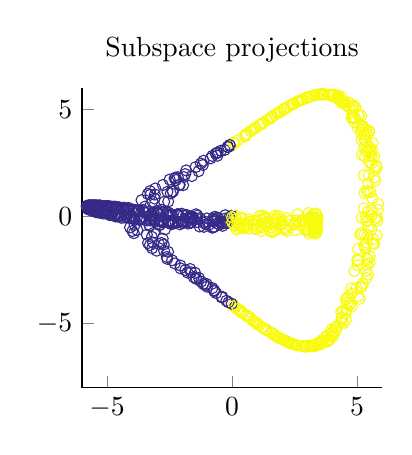
\begin{tikzpicture}

\begin{axis}[%
width=1.5in,
height=1.5in,
scale only axis,
colormap={mymap}{[1pt] rgb(0pt)=(0.2081,0.1663,0.5292); rgb(1pt)=(0.211624,0.189781,0.577676); rgb(2pt)=(0.212252,0.213771,0.626971); rgb(3pt)=(0.2081,0.2386,0.677086); rgb(4pt)=(0.195905,0.264457,0.7279); rgb(5pt)=(0.170729,0.291938,0.779248); rgb(6pt)=(0.125271,0.324243,0.830271); rgb(7pt)=(0.0591333,0.359833,0.868333); rgb(8pt)=(0.0116952,0.38751,0.881957); rgb(9pt)=(0.00595714,0.408614,0.882843); rgb(10pt)=(0.0165143,0.4266,0.878633); rgb(11pt)=(0.0328524,0.443043,0.871957); rgb(12pt)=(0.0498143,0.458571,0.864057); rgb(13pt)=(0.0629333,0.47369,0.855438); rgb(14pt)=(0.0722667,0.488667,0.8467); rgb(15pt)=(0.0779429,0.503986,0.838371); rgb(16pt)=(0.0793476,0.520024,0.831181); rgb(17pt)=(0.0749429,0.537543,0.826271); rgb(18pt)=(0.0640571,0.556986,0.823957); rgb(19pt)=(0.0487714,0.577224,0.822829); rgb(20pt)=(0.0343429,0.596581,0.819852); rgb(21pt)=(0.0265,0.6137,0.8135); rgb(22pt)=(0.0238905,0.628662,0.803762); rgb(23pt)=(0.0230905,0.641786,0.791267); rgb(24pt)=(0.0227714,0.653486,0.776757); rgb(25pt)=(0.0266619,0.664195,0.760719); rgb(26pt)=(0.0383714,0.674271,0.743552); rgb(27pt)=(0.0589714,0.683757,0.725386); rgb(28pt)=(0.0843,0.692833,0.706167); rgb(29pt)=(0.113295,0.7015,0.685857); rgb(30pt)=(0.145271,0.709757,0.664629); rgb(31pt)=(0.180133,0.717657,0.642433); rgb(32pt)=(0.217829,0.725043,0.619262); rgb(33pt)=(0.258643,0.731714,0.595429); rgb(34pt)=(0.302171,0.737605,0.571186); rgb(35pt)=(0.348167,0.742433,0.547267); rgb(36pt)=(0.395257,0.7459,0.524443); rgb(37pt)=(0.44201,0.748081,0.503314); rgb(38pt)=(0.487124,0.749062,0.483976); rgb(39pt)=(0.530029,0.749114,0.466114); rgb(40pt)=(0.570857,0.748519,0.44939); rgb(41pt)=(0.609852,0.747314,0.433686); rgb(42pt)=(0.6473,0.7456,0.4188); rgb(43pt)=(0.683419,0.743476,0.404433); rgb(44pt)=(0.71841,0.741133,0.390476); rgb(45pt)=(0.752486,0.7384,0.376814); rgb(46pt)=(0.785843,0.735567,0.363271); rgb(47pt)=(0.818505,0.732733,0.34979); rgb(48pt)=(0.850657,0.7299,0.336029); rgb(49pt)=(0.882433,0.727433,0.3217); rgb(50pt)=(0.913933,0.725786,0.306276); rgb(51pt)=(0.944957,0.726114,0.288643); rgb(52pt)=(0.973895,0.731395,0.266648); rgb(53pt)=(0.993771,0.745457,0.240348); rgb(54pt)=(0.999043,0.765314,0.216414); rgb(55pt)=(0.995533,0.786057,0.196652); rgb(56pt)=(0.988,0.8066,0.179367); rgb(57pt)=(0.978857,0.827143,0.163314); rgb(58pt)=(0.9697,0.848138,0.147452); rgb(59pt)=(0.962586,0.870514,0.1309); rgb(60pt)=(0.958871,0.8949,0.113243); rgb(61pt)=(0.959824,0.921833,0.0948381); rgb(62pt)=(0.9661,0.951443,0.0755333); rgb(63pt)=(0.9763,0.9831,0.0538)},
xmin=-6,
xmax=6,
ymin=-8,
ymax=6,
title={Subspace projections},
axis x line*=bottom,
axis y line*=left
]
\addplot[scatter,only marks,scatter src=explicit,scatter/use mapped color={mark=o,mark options={},draw=mapped color}] plot table[row sep=crcr,meta index=2]{%
-2.60787473797246	-1.89353097304865	-1\\
3.39927121184668	-0.2127241052027	1\\
4.41748810521752	5.32713984263384	1\\
3.27265932492734	-0.19930752826863	1\\
-0.294831548382515	3.10247711297807	-1\\
-1.1431888969311	-0.289389920875094	-1\\
-4.59270268310663	0.429263277589879	-1\\
-5.74145950959545	0.32509562759741	-1\\
3.15296957416239	-6.0228385708794	1\\
5.43301782570218	1.14150135572891	1\\
2.15467256597889	-0.572011036983853	1\\
3.28005738277053	-6.05222929795441	1\\
-2.99691867322404	0.171380955480563	-1\\
-0.105611831575106	-0.0406820636188634	-1\\
5.39127860488802	-1.9453005265042	1\\
-0.00781505453269143	0.0264563626155428	-1\\
-5.75506490240723	0.485571644747433	-1\\
4.75853577024966	-3.36358085848135	1\\
4.34493539953902	-4.93219101876572	1\\
-1.53607199086818	-2.82950630535506	-1\\
-4.02066633775674	-0.0164497049164366	-1\\
-5.57217062662991	0.268073530990043	-1\\
3.01061676885025	-6.05762468875017	1\\
-1.84128657948165	-0.263592666930388	-1\\
-3.91815115823241	0.307256926232656	-1\\
-3.36930353429606	1.04829108107575	-1\\
1.62028731347007	-0.724398303675576	1\\
2.06199371827026	4.9841314293239	1\\
-3.29252459910635	-0.440365951458999	-1\\
-5.31429842371296	0.452386642430618	-1\\
-1.46105807441038	2.29847609826534	-1\\
4.82614087253059	4.58175917615552	1\\
-2.89203101597523	-0.403088429104468	-1\\
1.1665043807491	-0.678356615876165	1\\
5.18044736127888	3.57689488246718	1\\
-1.2372268724152	-3.04227067858999	-1\\
3.64863442940519	5.71929774780518	1\\
-3.52384606992788	0.197427892686114	-1\\
-0.582574810536959	-0.0567283274893227	-1\\
-2.76532761820283	-0.189864080179945	-1\\
1.71435585510502	-0.224960871578739	1\\
0.671705306469632	-4.66857773808164	1\\
-4.50841691235312	0.377514093810841	-1\\
2.47530993629752	-5.96952920483248	1\\
4.38830224687814	5.57158004381318	1\\
-4.77508326215896	0.408889575914534	-1\\
-4.32480994074077	0.410146053383851	-1\\
4.77101378809497	4.62270019917055	1\\
5.36139735646257	3.52606194762376	1\\
5.14071903268497	-3.31908410616606	1\\
-2.77390230941699	-1.03977814910441	-1\\
5.68997837888017	2.78837706098264	1\\
0.872002117383234	-0.330655780351168	1\\
-4.63181002443573	0.398461593066273	-1\\
-5.6180961632065	0.369829467326594	-1\\
2.84708712166767	-6.0571246248529	1\\
-0.179280230421531	3.24427647039436	-1\\
3.1254215874739	-6.04521080727823	1\\
1.36361323707924	-5.27425643478073	1\\
4.24589732508257	5.63757088235391	1\\
0.33371941586145	-4.42875586962548	1\\
1.40851111015555	-0.311501138611116	1\\
5.40300527400355	1.19741279033875	1\\
-1.92762210700149	1.8378341204385	-1\\
-1.95002825478404	0.0431462888683706	-1\\
1.22668553139606	4.36280338415929	1\\
-5.6075357123484	0.488187084560207	-1\\
5.26912442807561	1.92074975573326	1\\
5.27760644629782	0.377041265282048	1\\
3.38283809042326	-0.731140738578153	1\\
5.29679469451516	-1.3378131090212	1\\
1.09830750362916	0.0138615864245848	1\\
0.265331446724561	-0.525503769327291	1\\
-3.8437418162801	0.282960482663516	-1\\
0.912553208249669	-0.584685449936046	1\\
2.06616954824032	-5.76531715822969	1\\
-1.4018445927636	-0.106373268820418	-1\\
3.41212560397713	-5.92690662094974	1\\
-1.01558924141789	-3.15350551850824	-1\\
4.78606128868967	-4.20179209475563	1\\
3.34371986877806	-6.03847396963077	1\\
1.88860900540522	-5.67592690590077	1\\
-3.35985102012431	-1.24039047567197	-1\\
-2.51279497619801	0.0797266039002044	-1\\
-4.45728920859996	0.041597046740857	-1\\
-4.6003144139374	0.404565752938079	-1\\
5.44338323514626	1.53548516452957	1\\
-4.49334167626446	0.416391389556623	-1\\
5.034572002678	4.13373306876785	1\\
0.592224559627323	-4.61926150350392	1\\
4.08706428203119	5.65362596247103	1\\
-4.03618412941241	0.317619253430122	-1\\
-3.34303330026304	0.205374062888811	-1\\
2.4287843104492	-5.95800701066506	1\\
-5.78719611793044	0.461997434027252	-1\\
1.5852259701768	-5.44579929508411	1\\
-3.8973932609645	-0.394333714466342	-1\\
4.84018499129863	4.6497628614482	1\\
5.17674391361598	4.05816630805377	1\\
-0.577194503830674	2.98425325494309	-1\\
3.58333640458623	5.69538135474434	1\\
-5.79293724889496	0.457382406247473	-1\\
5.00901467213698	-2.00924704458468	1\\
-1.33805569199511	2.11107950146837	-1\\
5.10241443465665	-3.8460155894408	1\\
2.53974972771702	-5.9953415659282	1\\
-5.74157710837594	0.337437381904843	-1\\
0.870011345344277	-0.42107878515261	1\\
3.05895268239201	-0.668040091961834	1\\
-2.65038841788895	0.102415202660548	-1\\
-0.41834781895291	-0.252319079919879	-1\\
-5.76100232136105	0.397734435357164	-1\\
0.391697053346456	-0.403702072862774	1\\
-0.167332521916148	-0.301615701653647	-1\\
2.32177390135925	-0.191901971871842	1\\
4.39727536821001	-4.70979384815806	1\\
-2.59220688733362	-1.97848873742016	-1\\
-5.76695614623623	0.472347054309741	-1\\
5.2026618765076	2.87582131459624	1\\
4.00452838648449	5.61788979491118	1\\
-5.42508057365113	0.5184816613008	-1\\
-5.08574138000045	0.480858112066519	-1\\
0.0307703852281559	-0.27274013282987	1\\
5.43899857236633	-2.71945836513702	1\\
5.69804178006896	1.81480044209181	1\\
-2.68099433620261	-0.604202465073557	-1\\
-5.35682736579542	0.18770991769961	-1\\
-1.79359910196981	-0.222873830425692	-1\\
1.70595677729194	4.73739796037682	1\\
4.44796955474093	-4.98381099192908	1\\
0.837271493669627	-4.87300159365032	1\\
-4.70111542740802	0.0439402755916172	-1\\
3.04678021833085	5.57007408161407	1\\
1.58156724467223	-0.343301644853889	1\\
3.37266718967562	-0.495404214651999	1\\
-4.53018077834775	0.0367343162851278	-1\\
5.23586728556984	4.21366266965044	1\\
3.75522921314646	-5.85171703886524	1\\
-4.60005141216782	0.405444464304827	-1\\
5.78243725787278	-0.875192012997742	1\\
-2.2399963317269	1.70058807076192	-1\\
-2.80718763390055	-0.271645124786655	-1\\
-5.00639599914105	0.144411241416207	-1\\
5.17224773403713	4.70139769036487	1\\
3.24168948398496	0.0871414449863895	1\\
5.69412721570869	-1.27785675198355	1\\
5.57636781822339	0.0468431316890742	1\\
1.1388947588949	-0.451968453950604	1\\
-1.04472327145216	-0.367638544296729	-1\\
3.5246111592604	-5.87888304147104	1\\
1.79474521587976	-5.62068574158788	1\\
3.03055628782519	-6.03028897309256	1\\
-0.371164383364573	-0.234407546866405	-1\\
1.19703168508384	-0.181520400300352	1\\
-5.79742893454697	0.460877875704554	-1\\
-5.80837500326389	0.498528757465795	-1\\
3.94354461624255	5.66236023731921	1\\
-5.55557893127096	0.355822614661628	-1\\
-3.40772352496615	-0.190568502020553	-1\\
1.55212663101554	4.60630319735481	1\\
-2.7139042636407	0.687649838624415	-1\\
-5.26510314399982	0.452925240309928	-1\\
3.46934849704483	-5.91750561039565	1\\
5.16048712292421	3.91810524728116	1\\
0.0665642485385554	-4.15286076859329	1\\
5.79175108839691	2.29170182004609	1\\
0.561688171468859	-0.408305688740578	1\\
-5.2673914108818	0.491482539558729	-1\\
-5.35602791787572	0.228239289085423	-1\\
0.388175845906234	-0.0597574854989457	1\\
3.55693424011506	5.70764367371422	1\\
-5.61544280688446	0.332487649321936	-1\\
3.25720645026975	-0.131587679959653	1\\
-3.8903582514402	-0.158780945849451	-1\\
4.42956487247186	5.29625219737199	1\\
0.390807212944238	-0.123272181463553	1\\
4.14788771508706	-5.34515038122469	1\\
0.134681779493251	-4.25951749270521	1\\
-5.78646155503314	0.442159849314659	-1\\
1.19519178212504	-5.16906588406715	1\\
-0.0795247846914519	3.288852818906	-1\\
4.37673458161497	5.42776234025887	1\\
-5.77795912559438	0.483219634106207	-1\\
5.29337854709386	3.20346198027424	1\\
-5.0271264336427	0.476967597262659	-1\\
3.36323812333214	-0.398438436279874	1\\
-2.76570566764327	1.46679057949542	-1\\
4.5640206457886	-4.35802010053728	1\\
-5.58458163845412	0.260519783880181	-1\\
-5.45110438712017	0.259994781984036	-1\\
1.83140273696539	4.83314192933478	1\\
-2.01075111068141	0.127521313234163	-1\\
5.18797339790989	-0.057410393449365	1\\
-1.64864545967794	-0.119492669449917	-1\\
0.673671682555094	-0.143224341153946	1\\
-3.48157926926895	0.457060047724352	-1\\
2.95860209182265	5.52888212008116	1\\
2.97680343066345	5.53404564887128	1\\
-4.10708037368063	-0.0697339832909677	-1\\
3.86084396293468	-5.78493812339226	1\\
-4.42716874964298	0.04489641563908	-1\\
-1.38874701096848	-0.26650072507635	-1\\
-4.10478723394831	0.374799928787888	-1\\
2.29829857108351	-5.89768399458483	1\\
-3.69138812270955	-0.0878853185627544	-1\\
-2.11823984191515	1.46987195645708	-1\\
5.06363545343512	4.72761693309105	1\\
-3.90920076835059	-0.0836342721987562	-1\\
5.19442011937504	-3.25325149415299	1\\
0.962104997419751	-4.96688431973068	1\\
4.92046938414294	4.60563147153812	1\\
1.26357526956423	-0.302397811598381	1\\
-2.55330994786321	0.69884020407826	-1\\
3.59841360228928	5.70683018034968	1\\
-5.4540599707789	0.505064096830511	-1\\
0.237921900652168	3.55807804469862	1\\
-2.54647046654663	-0.196104097402239	-1\\
2.27138937719053	-5.87092123244535	1\\
5.72059762824673	-0.111720561738055	1\\
3.30447730711475	-0.106104212129305	1\\
4.98164616438889	-3.33088767776012	1\\
3.36719152239208	5.65734877687588	1\\
-3.08322951900753	-0.207639289526347	-1\\
0.854890373296802	-0.204882170036449	1\\
2.42253430382543	5.23624120628811	1\\
-1.68808358584805	-0.0440572865758503	-1\\
-5.20012410581779	0.478636705358507	-1\\
1.53904195344212	-0.696975246642543	1\\
0.250653432545364	-4.32952914268181	1\\
-5.80945416203123	0.460907393394712	-1\\
-3.90752804807906	0.17215790382051	-1\\
3.08462464961652	-0.7884082971308	1\\
1.77474776146582	-0.072440519188032	1\\
-5.59885331327951	0.489866607598185	-1\\
1.93892835353413	4.89410522146796	1\\
-3.40833577220047	-0.854081054770183	-1\\
5.5785075248046	2.83538569522636	1\\
-4.42597018198956	-0.0639397316018264	-1\\
-1.60636787091614	1.88722774823756	-1\\
3.43846040000707	-5.99958479541957	1\\
4.89519102410833	-2.55203699192155	1\\
-0.388810939705733	-3.75302269669306	-1\\
-5.64497645478938	0.479817100174724	-1\\
-2.15532828446474	0.0230974984523182	-1\\
0.191969235280154	-0.280400909281302	1\\
4.65190368393344	-3.73843372280102	1\\
-0.716110082053765	-3.48292761138001	-1\\
-5.79060896083269	0.446084378101131	-1\\
3.5749708052359	5.70188017494472	1\\
-3.79123671771888	-0.636482716862291	-1\\
-5.06070904110231	0.454235602452569	-1\\
3.25395463695243	-0.524098921250588	1\\
-5.12133657058168	0.20267290996796	-1\\
5.30570611563661	-0.825558359946717	1\\
-3.18980761933008	0.694164839162033	-1\\
-4.97439746720223	0.452635067726662	-1\\
-3.4469353652351	0.163893420186365	-1\\
2.52876775555404	-0.29699896391555	1\\
-4.22440451481458	0.34209441217733	-1\\
0.518457584711596	3.73027404310538	1\\
-4.74074160333212	0.441549928438227	-1\\
-5.63127394643917	0.47868541670827	-1\\
3.49071004625276	-5.88518795867351	1\\
-3.71410512202791	0.24390531717458	-1\\
2.16707550332538	-5.83653261923906	1\\
-2.06369695208648	-2.29461883290352	-1\\
5.60159604959299	3.12056675798345	1\\
1.57537867358017	4.61559723681233	1\\
-4.42459904182307	0.378607925399097	-1\\
-0.851858549115274	2.71342591665154	-1\\
-5.20802461410092	0.245097975181433	-1\\
2.5727641942675	-0.178697116394646	1\\
4.85839834188358	5.10312488360973	1\\
3.39427785538786	-0.601158636549472	1\\
-1.48225103960064	-2.62829498219169	-1\\
-2.47430765123449	-0.222682982187031	-1\\
-2.37894130356819	1.1762912477022	-1\\
-0.788442589319612	2.82654710712773	-1\\
-0.270757676794192	0.0577821199075781	-1\\
2.97834673281096	-0.561212279218785	1\\
-3.11625173547502	-0.756135896797055	-1\\
-2.40129836086545	-0.293432189070819	-1\\
-3.57664359471249	0.300918933262423	-1\\
5.12267130786754	-0.834065576146642	1\\
-5.43605016191133	0.199341231088578	-1\\
4.0120735586326	5.66972773818391	1\\
2.27093940157133	-0.214040285424397	1\\
5.38912138839961	-1.22128621878061	1\\
-5.52267226760826	0.51300096591933	-1\\
5.36990868901424	-2.5467441382265	1\\
5.4513142545989	-0.503170688838256	1\\
4.85898130748363	4.97660484848261	1\\
-5.62895467916322	0.373140714423451	-1\\
0.747293018909135	3.98592322534806	1\\
1.76588365416509	-0.13751914744376	1\\
5.18738404779657	-0.775129302029753	1\\
-1.16923155253368	2.39913685548584	-1\\
1.67925088555112	-5.52558858030708	1\\
0.135097974180498	-0.435440174410464	1\\
-3.29321561561297	-0.417628403953682	-1\\
5.42490394275782	0.202589069964326	1\\
0.317824909447427	-0.404674740462509	1\\
3.36256419120486	0.13443343639887	1\\
1.50934012597747	4.55670951305019	1\\
5.53519216833315	1.14252247573739	1\\
-1.87365373534012	1.97642676004373	-1\\
-2.82695992379079	0.311343957696763	-1\\
-2.90321380618832	-0.394294680467798	-1\\
5.42919155806386	-0.864891004796046	1\\
3.38442257156649	-0.220407679109176	1\\
0.468675812599031	-0.544344973523526	1\\
1.41659760237479	4.50102542106478	1\\
-0.784311499770092	-0.211879145315471	-1\\
4.1753312266997	5.57308693707411	1\\
3.1119279530886	-6.04316821499759	1\\
-3.77845683095974	0.284243135989734	-1\\
-2.5905168107252	-0.264079374315844	-1\\
-2.71766777556759	-1.59758131178567	-1\\
2.93588947933512	-0.650402901502443	1\\
4.69599186613431	-4.14442089237161	1\\
-5.26974979213231	0.183531476681426	-1\\
3.42321768986558	-0.136349391828678	1\\
-2.80541114401062	0.198377696318948	-1\\
-0.640729642743601	-0.0920279128788086	-1\\
3.32805490349554	-0.166896322259807	1\\
2.10103281226447	5.01784742081151	1\\
0.517765233279387	3.79920497305656	1\\
3.27081294201401	-0.765997406571172	1\\
-0.593276491375492	-0.323341099915156	-1\\
-1.95628202380425	1.45880389978831	-1\\
-5.77414588430188	0.365514054464733	-1\\
-1.6340496197166	-0.297397099581427	-1\\
-4.40251322801745	0.379000587999403	-1\\
-5.7261492243648	0.400265273985575	-1\\
-5.66234787137542	0.36471703679838	-1\\
-5.79301283362604	0.464316811518456	-1\\
-3.11873101931291	-0.210940093865384	-1\\
0.104157551137585	3.40702463605621	1\\
-3.68587016859191	-0.0944500966887599	-1\\
4.65698301579559	5.3158392314563	1\\
-3.20476245437271	-0.953987007699295	-1\\
5.33888703634813	-1.50552215509435	1\\
4.38819586020516	-4.78280924657636	1\\
-5.01212460953436	0.439682521447785	-1\\
-1.63582750144281	-0.270284756200417	-1\\
-3.10036223142095	0.834606883167048	-1\\
-4.87531123299372	0.100497676677631	-1\\
-1.32475423435558	-2.8716693830533	-1\\
0.994809845927572	-0.189865312627241	1\\
-4.82590047046765	0.123505231871143	-1\\
5.8292024849355	0.308970275310249	1\\
0.58006772223721	3.8537828698038	1\\
-3.08879577790438	-0.137778495769082	-1\\
-3.97343690254122	-0.0952985004863442	-1\\
-0.60320118921734	2.96348090629922	-1\\
-4.54876423167054	0.0311698223835589	-1\\
5.44928584963781	-0.196444490116672	1\\
-2.49443121180136	1.72000501901839	-1\\
-0.716111876012625	-0.479865910387116	-1\\
1.83648634689228	-5.64436595223225	1\\
2.09298081843766	5.02349936484284	1\\
-5.37288918955467	0.265569929040952	-1\\
4.27115650767116	5.56939939394974	1\\
-0.415202784758911	-0.344697547049949	-1\\
-4.5941655544867	0.00545032531020031	-1\\
-5.41195148551339	0.295693188413346	-1\\
2.36035189222031	5.19410257964353	1\\
1.6806396340524	-0.689949281398725	1\\
5.3589082735687	-0.0035996807158663	1\\
3.60884525776394	-5.76953789818266	1\\
-2.29738928334383	1.77914360259063	-1\\
3.6868789355052	5.69192880063371	1\\
-1.58825361812879	-0.0854304357987424	-1\\
5.49127992794552	3.22691165950978	1\\
-5.7153907363857	0.51792760130266	-1\\
3.25475396526896	-6.04186669890753	1\\
-5.76169201254624	0.425542378885354	-1\\
0.051997394082158	3.44343624588074	1\\
-2.34566784435427	-0.323688601234774	-1\\
-5.59427350868232	0.516738350655221	-1\\
-4.69033806674552	0.108086404688233	-1\\
4.0597834480031	-5.47401854493957	1\\
-2.15871961185597	0.110416752558387	-1\\
-5.32930531653929	0.508671627731781	-1\\
5.52837483390235	1.14359205967575	1\\
2.60075359057026	5.34885990740135	1\\
-4.67825074002462	0.455028900089696	-1\\
3.05666894518359	5.56878287147968	1\\
3.17270716227273	-0.141877269898672	1\\
-2.46009383571491	0.10538923854895	-1\\
1.61403755732269	4.66761325178959	1\\
3.8711251906122	5.67253756028552	1\\
-1.50522450389874	-0.155951313597699	-1\\
-2.09315966405846	1.47809372510219	-1\\
3.33245702123292	-0.802918767667192	1\\
-1.6253115503543	-0.0247420676196523	-1\\
-0.441479181187212	3.07008779808267	-1\\
4.12045945071164	-5.19782799876563	1\\
-5.63262357977911	0.348138851221107	-1\\
5.39393973181798	-2.23351088984779	1\\
-2.824590605014	-1.23655976480635	-1\\
-1.44350564731102	-2.89174977922259	-1\\
4.27549637988034	5.58979183624764	1\\
1.10595715905876	4.2704057472011	1\\
-4.81089230400033	0.453165178858876	-1\\
-3.62006317145138	-0.14466095460419	-1\\
2.62056521272051	5.36187944146483	1\\
-3.93026446929606	0.272931110058631	-1\\
0.966306098892	4.15754490283658	1\\
0.898110190781989	4.09879819194782	1\\
0.176067613324209	-0.109743170370492	1\\
-1.91497697148705	-0.263528470600683	-1\\
2.4506615561056	5.25593500714696	1\\
-2.9997442418099	0.130828603752084	-1\\
3.4988524984361	5.6979658811739	1\\
-5.21764321124093	0.487508833853586	-1\\
-3.08830612418082	1.02255522667547	-1\\
-3.92858665070626	-0.779802620496754	-1\\
5.50982479110934	-1.86150104849703	1\\
-5.61452115058256	0.324359021862862	-1\\
3.42181181108634	-0.0307839458157573	1\\
4.78346545406072	-3.61423872490895	1\\
-2.2634104446103	1.81093303678799	-1\\
-5.27962113900629	0.502438561160313	-1\\
5.79537101680268	-0.0431859478696015	1\\
-1.83158995613089	2.14749018637144	-1\\
-2.36178942756853	1.16079535711574	-1\\
5.57069911755492	-0.62872303433696	1\\
4.8701661121658	4.58740086498963	1\\
5.55109854129987	2.99925869627546	1\\
-4.64675198488011	0.430145992296586	-1\\
-2.14537330879891	0.0763301266175464	-1\\
3.59837043472805	-5.81646506038081	1\\
3.13369010920328	-0.0274683677465507	1\\
-0.298785848494374	-0.114140517240798	-1\\
5.06469612417409	4.71964243478632	1\\
1.24219675384389	-5.20255721239658	1\\
2.19706078243348	-0.0842421255708505	1\\
-2.74405197738833	0.200353327311249	-1\\
-5.71133953357299	0.513632614698265	-1\\
-0.923512392954644	-0.381930963009365	-1\\
-3.15746649224172	-1.21778869135484	-1\\
-0.649632770191139	2.92826186064106	-1\\
-3.48068604561966	0.187006942651819	-1\\
-4.78152714645554	0.399512024380517	-1\\
-0.0945513353509298	3.33557152050965	-1\\
-5.73980541064647	0.360506963539846	-1\\
-4.94906304724514	0.125100807976695	-1\\
0.624924108589672	-0.407040025985877	1\\
3.5713156852414	-5.95882468328434	1\\
5.70841478201803	2.16706160361028	1\\
1.15511683899493	-0.427459852336507	1\\
4.37974589201764	5.33057536034515	1\\
-1.13028956844103	-0.48494779313973	-1\\
3.61467070235767	5.70723071421109	1\\
3.33820306538589	-0.608947634646196	1\\
-2.15376680418409	-0.242080935051842	-1\\
-0.223462789628109	-3.93481921896813	-1\\
-5.46979173293271	0.489404814152276	-1\\
-5.66816277195358	0.507964751475081	-1\\
-4.88880423766945	0.0604675996816257	-1\\
-1.77991381473124	-2.61999359428111	-1\\
3.29262059560776	5.63999379166959	1\\
5.38302199801894	-2.87932673351564	1\\
4.5420573491262	-4.53187902185909	1\\
4.50802967108701	5.33951196495121	1\\
5.0204618825	-2.27833670935264	1\\
-2.99408663562005	0.147901783611429	-1\\
2.80706672291416	-6.05694256781373	1\\
0.30333803168371	-0.435498057698326	1\\
3.279114193022	5.64375000027127	1\\
-0.246253328122132	-0.289806991706455	-1\\
-3.65728102848068	-0.0892227853937421	-1\\
5.38679148726828	3.85642947520302	1\\
2.21251933837462	-5.84789349334305	1\\
-5.76090076625014	0.457464620993806	-1\\
-5.13494645046668	0.135193178921761	-1\\
-5.632931938499	0.355193080515412	-1\\
-3.60920140827916	-0.0778326952531975	-1\\
0.975336121375006	-0.578926470133526	1\\
5.31153369423589	-1.42214071832703	1\\
3.36787599409786	-0.160430431888652	1\\
3.75297584500313	-5.64683254069088	1\\
-2.94965752636126	-0.218592480442353	-1\\
-0.63676497900035	-3.57734335750456	-1\\
5.49709842891201	-2.17608179164807	1\\
2.79754976454547	5.44684015487548	1\\
-3.98489731966972	-0.680605970426286	-1\\
4.47301628966458	5.3441655915436	1\\
5.2877478595196	3.81693349645674	1\\
2.29441074773175	-0.406440289198395	1\\
-2.56044535742116	-0.225760984556172	-1\\
-4.24256320217553	0.0123107326838462	-1\\
-4.21181465629812	-0.0183666638252301	-1\\
3.06577456266471	0.162420755266784	1\\
-5.77344522805774	0.46063605301285	-1\\
-2.61305869589274	0.121830186003011	-1\\
-1.2461087423554	2.46841061280806	-1\\
-2.0883529586992	-0.367635801761362	-1\\
-4.52363685002185	0.415459842021389	-1\\
4.19035271791775	-5.14365073076566	1\\
2.62336051004997	5.36025025323428	1\\
0.404771054438753	-4.48321673049925	1\\
3.99227774532645	5.67828175320831	1\\
1.84496625886237	0.0186178465587736	1\\
-5.77212815186076	0.419181535697806	-1\\
5.72994191145256	1.65789346435488	1\\
-2.58394412975409	1.15047146669671	-1\\
-4.84725375572436	0.109164974235321	-1\\
-0.68627150138057	-0.0152446628733955	-1\\
2.54364081132177	-0.639007331718617	1\\
-4.98589815745471	0.182163509692005	-1\\
-0.789016538473669	-0.524892258079828	-1\\
0.746970254260457	3.97948529088389	1\\
-3.28085007338415	1.18077922394596	-1\\
5.63756208201821	-1.05688575768549	1\\
1.66129144411695	-5.51344814209584	1\\
-4.45344296122414	0.0619844935322056	-1\\
5.43409305535211	-1.99125029551146	1\\
4.24849913294288	5.47526725757596	1\\
-2.54969020236805	0.176754901411414	-1\\
4.71035399615254	-4.06735274361007	1\\
1.93550114760506	4.90168645734484	1\\
1.82487071535928	4.82166798142719	1\\
-1.00173153460482	-0.0932370677662765	-1\\
5.48550716179874	2.51565612972354	1\\
-3.7550228857281	0.270272454210525	-1\\
1.37308595692611	-0.434454188049545	1\\
3.29565874831682	-0.582760311179173	1\\
-0.37957709158939	-0.437432417997082	-1\\
-5.65704751462205	0.478692066355253	-1\\
-1.42262925613477	-2.91540188429074	-1\\
-1.29767373586905	-0.468374950847031	-1\\
1.23993296426263	4.37294833410529	1\\
-4.19440822987888	0.311398256871821	-1\\
2.6181169097625	-6.01785355239859	1\\
0.577843151515631	-4.63167671531069	1\\
-1.55841705010323	-0.0349026651992161	-1\\
2.47056992444446	5.26965270881705	1\\
4.02872865136486	-5.3964790490133	1\\
-5.79101194683389	0.43696006071306	-1\\
-0.156820442096793	3.24175669070301	-1\\
-5.53237360184242	0.250317772121929	-1\\
-5.36218815960628	0.285253621349758	-1\\
-5.79139201594798	0.454423213976665	-1\\
-5.66366785531634	0.497307383454774	-1\\
-4.80114719791385	0.0648042642371041	-1\\
-5.05710897607158	0.195587824342475	-1\\
-3.08297445950886	-0.152761441573155	-1\\
2.09158452150135	-5.79208922878247	1\\
4.27914009623491	5.53875503728422	1\\
-1.97054286024783	-0.216594445227255	-1\\
3.19405366678966	-0.368312930648139	1\\
5.82013773931093	-0.202959697732833	1\\
-3.56777912533883	-0.0131092261297021	-1\\
-5.42642432510752	0.220991528210838	-1\\
-1.73745426973386	-0.0518774124151211	-1\\
-2.73201390333369	-1.30940624148129	-1\\
3.38939721292471	-0.54532192784904	1\\
0.183990917594044	-0.608553897405053	1\\
0.824831683893197	4.04181103062059	1\\
5.58945032599002	2.48899830329062	1\\
-5.76464064260332	0.491908800738571	-1\\
-3.01187215007005	-1.59645877154339	-1\\
5.84330509093925	0.583433240093333	1\\
-5.79607498303022	0.477427339508157	-1\\
5.64553779682603	-1.24793044194533	1\\
2.68841745317554	5.39813600478865	1\\
2.75620332331482	5.42632479346217	1\\
-4.67627203040496	0.051461134732935	-1\\
-1.28696105838186	-0.0833549962479631	-1\\
-2.80776058474315	-0.225791232258208	-1\\
5.25752334541098	4.12396925623912	1\\
5.47068858174932	3.94491255706625	1\\
-2.82606884204541	-0.222003845118927	-1\\
0.0977581658189957	-0.407628977461607	1\\
3.83371403308856	-5.82429367446339	1\\
4.6811862526031	5.10818928601616	1\\
1.79820371660721	-0.614845384385121	1\\
1.0230860821124	-5.03032514477611	1\\
-5.79387745651748	0.447391304276653	-1\\
-0.138618868054978	-4.00885025586611	-1\\
2.59988718324779	-6.01332575335519	1\\
1.75917959035573	-0.371800005121845	1\\
-5.79810762536415	0.449332934692008	-1\\
4.55402620993577	-3.86629927016084	1\\
-3.26333358461636	1.01408192339769	-1\\
1.98911698445319	-0.353910199307466	1\\
2.2100433166862	-0.690053209725387	1\\
2.67791981727095	5.39030342398509	1\\
-3.19685939028579	-1.48176337370473	-1\\
-0.741274888739338	-0.502409590763382	-1\\
5.35325009696065	4.078083221631	1\\
2.95176419588393	-6.05849176650116	1\\
-2.45132895534443	1.07707519387481	-1\\
2.36407508970119	-5.92546579689532	1\\
-1.97790550610352	-0.307765653427579	-1\\
-3.27481071058134	-0.17958054121302	-1\\
4.29229798060418	5.46328754432076	1\\
5.50450478090434	2.82966963615254	1\\
3.95467586157216	-5.57768053220588	1\\
-2.917978023231	0.160949968553693	-1\\
-1.05235889466838	-0.249960176862605	-1\\
-2.01621871159271	-0.305054578540042	-1\\
-3.28526475684605	-1.3421063649939	-1\\
5.51356284723643	3.09512145290084	1\\
-2.89611971513263	-0.197335655411923	-1\\
1.32286633036529	-0.0893347669098846	1\\
3.41300217418166	-0.362315403987953	1\\
2.97334895071128	5.52726370235942	1\\
5.47708880242262	3.99974885126012	1\\
3.90704261377483	-5.72970959561818	1\\
4.57156868263435	5.19291546950928	1\\
1.72249013313128	0.0417384798828536	1\\
-5.70207537138681	0.362347674816648	-1\\
4.82277673458183	5.1943147370464	1\\
5.58453713275678	0.280025611758876	1\\
3.40661212282488	5.67220436165282	1\\
-2.26279303763698	-0.251088794196709	-1\\
-4.60761489061975	0.412976886332619	-1\\
3.13577310485814	-0.48667676091017	1\\
0.341880302439502	-4.40192545470424	1\\
1.16454175538614	4.29388126885025	1\\
2.21878754310057	5.09312400738237	1\\
-5.53355464307764	0.511965319487245	-1\\
-4.31523223280974	-0.0457315245310233	-1\\
4.89212992443119	4.40231088595472	1\\
-1.38449866673633	0.0390469498179418	-1\\
-1.07463096685091	-3.19991287781409	-1\\
-2.17980867308399	0.100874797592717	-1\\
5.23735388834896	-3.12914694329786	1\\
0.635829987863897	-0.57126953854309	1\\
-3.13068339797684	0.173712435017811	-1\\
-3.07058211593192	-0.135501199461253	-1\\
1.32249406868291	-0.0219685082809125	1\\
-5.75337089931824	0.429584039945615	-1\\
2.7867645426783	-0.160168332988659	1\\
-2.88632441985171	0.0828386830859857	-1\\
5.30054841465491	3.57711006990099	1\\
1.75584754562777	-5.59016349091032	1\\
2.68666987431897	-0.266798117341575	1\\
-1.95714333677243	-0.212704047184104	-1\\
-3.00219957039393	0.238414254302886	-1\\
4.05709654284638	5.66190466765346	1\\
2.67724020114224	-0.401210669381031	1\\
-5.25833250736174	0.229581150492868	-1\\
4.93018256061751	5.10303648974087	1\\
-1.63594505601648	-2.61155813423949	-1\\
2.62490976964067	0.0978088542401988	1\\
-5.76705273054466	0.470216249086984	-1\\
-4.92509290361529	0.476408894993284	-1\\
2.95668364790766	-0.586942473259849	1\\
-1.44100182098845	0.09945246308573	-1\\
3.39041586370757	-0.713879549554918	1\\
0.903659216054335	-4.91685388081837	1\\
-4.88628458677546	0.455618399682261	-1\\
-3.72098278716319	-0.142262802223876	-1\\
-3.9302737686963	-0.0501132099823897	-1\\
5.47542473291786	1.93050778223891	1\\
4.0330214933563	-5.58747318536443	1\\
-4.07866209487916	-0.511475155097257	-1\\
1.26398443474776	-0.105282622659175	1\\
2.1184571353436	-0.618809438653947	1\\
-1.866922959181	-2.50287093259494	-1\\
-5.78264163648194	0.438419055880785	-1\\
-2.56431581810952	0.186387547173891	-1\\
-4.8073229244511	0.446345167271075	-1\\
1.56785568560806	-5.41684933013919	1\\
-2.35846951602619	-0.274002937492155	-1\\
-2.06190412021024	-2.42320166031872	-1\\
0.979102388478552	-4.96110754607861	1\\
3.75815020154914	-5.59315947885786	1\\
3.34706741676708	0.119092018252974	1\\
-1.83347314725068	0.071980856672709	-1\\
-3.13335239233617	-0.211781448675738	-1\\
-4.5239526473842	0.354531881170705	-1\\
-2.39859024947776	-2.04420195598676	-1\\
-5.55718996716969	0.501971038765079	-1\\
-4.78209721238232	0.136036370096119	-1\\
-1.14977006437037	-3.15056465056481	-1\\
-4.99355684122379	0.173631756844233	-1\\
4.17891871321676	-5.15037297091505	1\\
-0.59934419713974	-0.198663194086265	-1\\
1.98175284074383	-5.72031111847064	1\\
2.8318179934336	5.46173254384607	1\\
0.0589593706510263	-4.19407616743012	1\\
3.20958591518866	-6.05572523227697	1\\
-0.536023671954733	-0.35977373672074	-1\\
5.18048602999907	4.20838386278146	1\\
-5.77381914219781	0.457264625031415	-1\\
2.00028779775274	-0.177411315315553	1\\
5.61256562854197	0.844892514594805	1\\
2.83654062046955	-0.218703099384144	1\\
2.52072488727806	-0.36259357878968	1\\
4.61730209720132	-4.01364123891661	1\\
4.44505647088896	-4.39009033322071	1\\
-0.0124705433633143	-4.07627130999073	-1\\
1.93563122611444	4.90426074319007	1\\
-4.34562528496742	0.34154420569539	-1\\
-4.32377988305421	0.365734940754748	-1\\
-1.67473126299011	-2.45465133535956	-1\\
0.00430924843198379	-0.0447369260586298	1\\
-5.63083415867065	0.504620762818402	-1\\
5.39702694053205	3.01198696171382	1\\
-3.06899866030679	1.3047641541586	-1\\
-0.491015773297071	-0.243198757129089	-1\\
-5.24486796058649	0.158164705653685	-1\\
4.03576870583263	5.66001537539407	1\\
3.13589119373899	5.60425160614459	1\\
-2.16854615753796	1.83030194894188	-1\\
-5.53279695246995	0.515706373057045	-1\\
-1.13771278100898	2.5984984493652	-1\\
-2.29013080649527	-2.19473669096261	-1\\
2.41172761012184	-5.94764631872321	1\\
0.666355107860024	-0.274043242181988	1\\
4.70826260214255	5.08695471202782	1\\
-0.715915669005644	-3.44239412948388	-1\\
4.36658276882692	-4.46937065065849	1\\
-4.98863392185683	0.491238967278158	-1\\
-3.6202690071454	0.75753506340633	-1\\
-5.36362224928763	0.272361075164853	-1\\
2.47616121531729	-5.96649216149608	1\\
5.29860612588796	1.08957133760238	1\\
3.21896621904353	-0.472602473472458	1\\
-4.75970836070982	0.444191948884355	-1\\
4.56021293723695	-4.83082696959586	1\\
-2.41429842512189	-0.36077054027338	-1\\
-1.81666259832001	0.0496649857732678	-1\\
0.444338540761597	-0.491960687037416	1\\
2.96681787570107	-0.215572724251069	1\\
-1.76066563033283	-0.329205712396706	-1\\
1.35825343128081	-5.30054470864999	1\\
5.76689830037547	2.37874309329057	1\\
1.20927395842539	0.0479136859040593	1\\
-0.417400635519561	-3.77802004020244	-1\\
5.03997696082845	-3.72958110413213	1\\
-0.787833144618972	-3.34645689738035	-1\\
5.31945621400762	2.78850676594344	1\\
-0.998447099837098	-3.27661195247175	-1\\
-4.5456069164829	0.0316352463866278	-1\\
1.71238507191714	-0.310101812418523	1\\
-0.585205296025636	2.83191959181891	-1\\
-0.670354217780958	-0.158994591319689	-1\\
-4.66389968030123	-0.000319418825051399	-1\\
5.37547580563178	-0.194621632516888	1\\
0.227162655676174	-4.3337929523133	1\\
-2.51926345205144	-0.312793461251409	-1\\
2.11585928087422	5.03731242180651	1\\
-2.40219192370245	0.0625422528306497	-1\\
-2.55977434323388	-1.65146941288739	-1\\
-1.63090475370419	-0.100282646468245	-1\\
2.83258101420361	-0.160459208951431	1\\
5.37284104461833	3.24966577748611	1\\
-5.21621750313261	0.188094843563324	-1\\
-5.49865361642352	0.466249313839622	-1\\
3.56686054784737	-5.86179609368491	1\\
0.122373021208394	0.0464505223230599	1\\
5.04371559498053	-1.51463370455524	1\\
-5.67846427948399	0.358317090022746	-1\\
4.58336956130282	-3.84571099144331	1\\
-3.92194418178623	0.27022578591429	-1\\
1.17504444665855	-0.505265080997279	1\\
-3.28216028763845	-0.177633688438859	-1\\
-0.734428482703698	-0.227866519103307	-1\\
-2.50966681364884	-0.259135902204275	-1\\
1.09119366824471	-5.08414055927313	1\\
-3.26678972639922	-0.112159622921684	-1\\
-3.23433475445363	0.0897344936107896	-1\\
-1.65067301396182	-0.000860206491715795	-1\\
5.62132800975007	3.43196614698675	1\\
0.00551014072912123	-0.269947181988889	1\\
0.431674327518581	-4.51818141821649	1\\
-5.27037843504369	0.505680726177656	-1\\
1.53517492188745	-0.519076284865955	1\\
3.10329093838736	-0.0969408441095232	1\\
-3.9069964236794	-0.0580276058890745	-1\\
2.96819250542171	5.53606356846944	1\\
3.25542327001429	-6.00220683803044	1\\
3.42499652602466	-5.95181664400849	1\\
-2.9191094408235	-1.28819996664168	-1\\
-5.35021008623556	0.500934152568511	-1\\
-5.10205806069458	0.1904997036878	-1\\
-0.760171870054939	-0.100065115952735	-1\\
3.9897783667157	-5.45780746063406	1\\
2.92304062474235	-6.07897012883676	1\\
-5.49356789386418	0.238111692760219	-1\\
0.754409977190016	-4.76576741049218	1\\
-5.23837595518162	0.231438739628738	-1\\
3.9884851464415	-5.25939878239823	1\\
1.38046489167288	-5.30376203300286	1\\
-2.56394254788912	0.0542225293902076	-1\\
3.09579156699577	-0.0934286845385086	1\\
-4.15192234230467	0.396661219373928	-1\\
5.05202599636482	-2.06922054079049	1\\
2.09578375518707	-0.509962225849396	1\\
-5.78555179799953	0.454125329402657	-1\\
2.45441674407931	5.25665152852165	1\\
3.15325949890755	-0.238570008879027	1\\
-5.7663758858557	0.45965937235861	-1\\
0.305234393133181	-0.358515331026994	1\\
};
\end{axis}
\end{tikzpicture}%
\end{document}
\caption{Spectral clustering and subspace projections using $\sigma^2 = 0.1$.}
\label{fig:clusteringResults}
\end{figure}


